\documentclass[12pt,a4paper]{report}
\usepackage[top=2.5cm, bottom=2.5cm, left=2.5cm, right=2.5cm]{geometry}

% Différentes options pour la classe :
% - taille de la fonte    : 10pt, 11pt, 12pt
% - recto ou recto-verso    : oneside, twoside
% - stade de développement    : draft, final

\usepackage[english]{babel}
%\usepackage[latin1]{inputenc}    % Pour utiliser les lettres accentuées
\usepackage[utf8]{inputenc}%           gestion des accents (source)
%\usepackage[T1]{fontenc}%              gestion des accents (PDF)
%\usepackage[francais,english]{babel}%          gestion du français
%\usepackage[utf8]{inputenc}
\usepackage{textcomp}%                 caractères additionnels
\usepackage[pdftex]{graphicx}
\usepackage{setspace}
\usepackage{hyperref}
\usepackage[french]{varioref}
\usepackage{fancyhdr}
\usepackage{color}
\usepackage{colortbl}
\usepackage{amsmath}
\usepackage{ifpdf} % part of the hyperref bundle
\usepackage{array} 
\usepackage[LGR,T1]{fontenc}
\usepackage{textgreek}
\usepackage{textalpha}
\usepackage[francais]{babel}
\usepackage{amsfonts}
\usepackage{amssymb}
\usepackage{abstract}
\usepackage{caption}     % better captions
\usepackage{subcaption}  % subfigures
\usepackage{pdfpages}
% set fonts for nicer pdf view
\IfFileExists{lmodern.sty}{\usepackage{lmodern}}{}
\pagestyle{fancy}
\fancyhead[L]{\nouppercase\leftmark} %pour afficher le nom du chapitre à gauche
\fancyhead[C]{}
\fancyhead[R]{\nouppercase\rightmark} %pour afficher le nom de la section à droite
\usepackage{float}
\fancyfoot[L]{}
\fancyfoot[C]{}
\fancyfoot[R]{\textbf{\thepage}}

% Début du document
\begin{document}

\pagenumbering{gobble} % Supprimer les numéros de page

%%%%%%%%%%%%%%%%%%%%%%%%%%%%%%%%%%%%%%%%%
% University Assignment Title Page 
% LaTeX Template
% Version 1.0 (27/12/12)
%
% This template has been downloaded from:
% http://www.LaTeXTemplates.com
%
% Original author:
% WikiBooks (http://en.wikibooks.org/wiki/LaTeX/Title_Creation)
%
% License:
% CC BY-NC-SA 3.0 (http://creativecommons.org/licenses/by-nc-sa/3.0/)
% 
% Instructions for using this template:
% This title page is capable of being compiled as is. This is not useful for 
% including it in another document. To do this, you have two options: 
%
% 1) Copy/paste everything between \begin{document} and \end{document} 
% starting at \begin{titlepage} and paste this into another LaTeX file where you 
% want your title page.
% OR
% 2) Remove everything outside the \begin{titlepage} and \end{titlepage} and 
% move this file to the same directory as the LaTeX file you wish to add it to. 
% Then add \input{./title_page_1.tex} to your LaTeX file where you want your
% title page.
%
%%%%%%%%%%%%%%%%%%%%%%%%%%%%%%%%%%%%%%%%%



\begin{titlepage}



\newcommand{\HRule}{\rule{\linewidth}{0.5mm}} % Defines a new command for the horizontal lines, change thickness here

\center % Center everything on the page
 
%----------------------------------------------------------------------------------------
%	HEADING SECTIONS
%----------------------------------------------------------------------------------------


\begin{minipage}[l]{0.2\columnwidth}

\includegraphics[width=3cm,height=3cm]{imagess/logo insat.jpg}\\
\end{minipage}
\hfill
\begin{minipage}[l]{0.5\columnwidth}
\centering
\footnotesize
\textbf{\textsc{REPUBLIC of TUNISIA}}\\
\textbf{\textsc{Ministry of Higher Education and Scientific Research
University of Carthage}}\\
\textbf{\textsc{National Institute of Applied Sciences and Technology}}
\end{minipage}
\hfill
\begin{minipage}[l]{0.2\columnwidth}

\includegraphics[width=3cm,height=3cm]{imagess/logo_universite_carthage.png}\\
\end{minipage}
\HRule \\[0.2cm]
\vskip1cm%

%----------------------------------------------------------------------------------------
%	TITLE SECTION
%----------------------------------------------------------------------------------------

\textsc{\large Graduation Project\\ to obtain\\ National Engineering Diploma\\
in Applied Sciences and Technology\\ Curriculum: Industrial IT and Automation
}\\[0.5cm] % Minor heading such as course title\\




\HRule \\[0.5cm]
\textcolor{black}{ \LARGE \bfseries Simultaneous Multi-frequency Electrical Impedance Tomography System for Biomedical Applications}\\[0.5cm] % Title of your document
\HRule \\[0.5cm]


 % Minor heading such as course title\\


\textit{Prepared by :}\\
\vskip0.5cm%
\textsc{\large \bfseries   Ichrak Khaldi   }\\[0.5 cm] % Minor heading


\textit{Hosted by Measurement and Sensor Technology professorship at Chemnitz University of Technology}\
\begin{figure}[H]
    \centering
    
\includegraphics[width=0.2\linewidth]{imagess/MST_logo.png}
\end{figure}

\begin{center}
\noindent
{\emph{Defended on the 25/09/2025 in front of a jury composed of:}} \\
\end{center}
% Jury Members 
\begin{center}
\begin{tabular}{ll}
Prof. Raouf Ketata & \textbf{President of the jury} \\
Prof. Feiza Ghezail & \textbf{Reviewer} \\
Prof. Olfa Kanoun  & \textbf{Supervisor at the company} \\
Dipl.-Ing. Bilel Ghoul  & \textbf{Co-supervisor at the company} \\
Prof. Salma Ben Said & \textbf{Supervisor at INSAT} \\
\end{tabular}
\end{center}

%\hfill




{\large\bfseries Academic year: 2024 - 2025}\\[0.2cm] 



\vfill % Fill the rest of the page with whitespace


\end{titlepage}


%\end{document}
%%%%%%%%%%%%%%%%%%%%%%%%%%%%%%%%%%%%%%%%%%
% University Assignment Title Page 
% LaTeX Template
% Version 1.0 (27/12/12)
%
% This template has been downloaded from:
% http://www.LaTeXTemplates.com
%
% Original author:
% WikiBooks (http://en.wikibooks.org/wiki/LaTeX/Title_Creation)
%
% License:
% CC BY-NC-SA 3.0 (http://creativecommons.org/licenses/by-nc-sa/3.0/)
% 
% Instructions for using this template:
% This title page is capable of being compiled as is. This is not useful for 
% including it in another document. To do this, you have two options: 
%
% 1) Copy/paste everything between \begin{document} and \end{document} 
% starting at \begin{titlepage} and paste this into another LaTeX file where you 
% want your title page.
% OR
% 2) Remove everything outside the \begin{titlepage} and \end{titlepage} and 
% move this file to the same directory as the LaTeX file you wish to add it to. 
% Then add \input{./title_page_1.tex} to your LaTeX file where you want your
% title page.
%
%%%%%%%%%%%%%%%%%%%%%%%%%%%%%%%%%%%%%%%%%



\begin{titlepage}

\newcommand{\HRule}{\rule{\linewidth}{0.5mm}} % Defines a new command for the horizontal lines, change thickness here

\center % Center everything on the page
 
%----------------------------------------------------------------------------------------
%	HEADING SECTIONS
%----------------------------------------------------------------------------------------


\begin{minipage}[l]{0.2\columnwidth}

\includegraphics[width=3cm,height=3cm]{imagess/logo insat.jpg}\\
\end{minipage}
\hfill
\begin{minipage}[l]{0.5\columnwidth}
\centering
\footnotesize
\textbf{\textsc{REPUBLIC of TUNISIA}}\\
\textbf{\textsc{Ministry of Higher Education and Scientific Research
University of Carthage}}\\
\textbf{\textsc{National Institute of Applied Sciences and Technology}}
\end{minipage}
\hfill
\begin{minipage}[l]{0.2\columnwidth}

\includegraphics[width=3cm,height=3cm]{imagess/logo_universite_carthage.png}\\
\end{minipage}
\HRule \\[0.2cm]
\vskip1cm%

%----------------------------------------------------------------------------------------
%	TITLE SECTION
%----------------------------------------------------------------------------------------

\textsc{\large Graduation Project\\ to obtain\\ National Engineering Diploma\\
in Applied Sciences and Technology\\ Curriculum: Industrial IT and Automation
}\\[0.5cm] % Minor heading such as course title\\




\HRule \\[0.5cm]
\textcolor{black}{ \LARGE \bfseries Simultaneous Multi-frequency Electrical Impedance Tomography System for Biomedical Applications}\\[0.5cm] % Title of your document
\HRule \\[0.5cm]


 % Minor heading such as course title\\

\textit{Prepared by :}\\
\vskip0.5cm%
\textsc{\large \bfseries   Ichrak Khaldi   }\\[0.5 cm] % Minor heading


\textit{Hosted by Measurement and Sensor Technology professorship at Chemnitz University of Technology}\
\begin{figure}[H]
    \centering
    
\includegraphics[width=0.2\linewidth]{imagess/MST_logo.png}
\end{figure}


\renewcommand{\arraystretch}{2}  % Increases vertical spacing
\begin{center}
\begin{tabular}{|c|c|}
  \hline
  \shortstack{Supervisor at the company \\ \textbf{Prof. Olfa KANOUN}} 
    & \shortstack{Supervisor at INSAT \\ \textbf{Prof. Salma BEN SAID }} \\
  \hline
  \rule{0pt}{40pt} & \rule{0pt}{40pt} \\
  \hline
\end{tabular}
\end{center}
\renewcommand{\arraystretch}{2}  % Increases vertical spacing


{\large\bfseries Academic year: 2024 - 2025}\\[0.2cm] 








\end{titlepage}


%\end{document}

\includepdf[pages=-]{Rapport_pfe__final___6_ (16) (1)-2.pdf}
\newpage
\chapter*{Dedication}
\setstretch{1.2}
\normalsize{}
\textbf{To my beloved parents Mouldi and Sassia},  
I owe you more than words could ever express. You have been my constant source of strength, love, and inspiration. You never left me to face challenges alone; instead, you stood by my side with patience and unwavering faith. You encouraged me at every step, provided me with everything I needed, and believed in me even when I doubted myself. Your sacrifices, unconditional love, and boundless support are the foundation upon which all my achievements rest. This work is, above all, a reflection of your endless devotion and guidance.  \\
\normalsize{}
\\
\textbf{To Iheb and Ibtihel},  
thank you for being more than siblings for being my lifelong companions, my confidants, and my motivation. Your encouragement, care, and constant support have been an anchor throughout my journey. Every success I celebrate carries a part of you, and I am endlessly grateful for the love and pride you have always shown me.  \\
\normalsize{}
\\
\textbf{To my dear friends Salwa, Khouloud, Nour, and Ons},  
who made this path brighter and easier, I owe countless moments of joy. I am truly grateful for every laugh, every conversation, and every moment of comfort we shared. You were my safe haven from stress and fatigue.  \\
\normalsize{}
\\
\textbf{To my KOSPIE family, Dorra, Feriel, Koussay, Salsabil and Farah},  
thank you for transforming my six months in Germany into a second home, filled with unforgettable memories, warmth, and true friendship.  \\
\normalsize{}
\\
Finally, \textbf{to everyone I have met at INSAT},  
thank you for making these past five years the most beautiful and memorable chapter of my life. Your support, companionship, and the experiences we shared have shaped me both personally and academically, turning this journey into a treasure I will carry forever. \\ 
\begin{flushright}
Ichrak Khaldi
\end{flushright}


\chapter*{Acknowledgements}
\setstretch{1.2}
\normalsize{}
I would first like to express my sincere gratitude to the\textbf{ Measurement and Sensor Technology Laboratory at Technische Universität Chemnitz}, which served as my host institution during this project, for providing an excellent research environment and continuous support.
\\
\normalsize{}
\\
My deepest appreciation goes to \textbf{Prof. Olfa Kanoun}, Head of the Measurement and Sensor Technology professorship, for her expert guidance, constructive feedback, and encouragement, which were essential in shaping the outcome of this work. I am equally grateful to \textbf{Dipl.-Ing. Bilel Ghoul}, my co-supervisor at TU Chemnitz, for his availability, assistance, and valuable insights that significantly contributed to the progress of this project.
\\
\normalsize{}
\\
I also wish to extend my heartfelt thanks to \textbf{Prof. Salma Ben Said}, my academic supervisor at INSAT, for her trust, support, and insightful advice throughout this journey. Her guidance has greatly enriched both the scientific and personal dimensions of my work.
\\
\normalsize{}
\\
Finally, I would like to thank the president of jury \textbf{Prof. Raouf Ketata} and the exam-
inator \textbf{Prof. Feiza Ghezail} for accepting to evaluate this thesis and for their valuable time, feedback, and contributions. My sincere gratitude also goes to all those who, directly or indirectly, provided their support, encouragement, and advice during the completion of this work.



\tableofcontents % Table of Contents
% Set front matter page numbering in Roman numerals
\pagenumbering{roman}


% List of Figures
\listoffigures
\addcontentsline{toc}{chapter}{\listfigurename} % ensures entry in TOC

% List of Tables
\listoftables
\addcontentsline{toc}{chapter}{\listtablename}  % ensures entry in TOC
\addcontentsline{toc}{chapter}{Acronymes}
\chapter*{List of Acronyms}
\addcontentsline{toc}{chapter}{List of Acronyms}

%%%%%% NB. Please ensure that the acronym list is maintained in alphabetical order.

\vspace{0.5cm}
\begin{itemize}
    \item \textbf{ADC:} Analog-to-Digital Converter
    \item \textbf{DAC:} Digital-to-Analog Converter
    \item \textbf{DAQ:} Data Acquisition
    \item \textbf{DMA:} Direct Memory Access
    \item \textbf{DSP:} Digital Signal Processor / Digital Signal Processing
    \item \textbf{EIT:} Electrical Impedance Tomography
    \item \textbf{FFT:} Fast Fourier Transform
    \item \textbf{FPGA:} Field Programmable Gate Array
    \item \textbf{GPIO:} General-Purpose Input/Output
    \item \textbf{HAL:} Hardware Abstraction Layer
    \item \textbf{I/Q:} In-phase / Quadrature
    \item \textbf{IEC:} International Electrotechnical Commission
    \item \textbf{MCU:} Microcontroller Unit
    \item \textbf{PCB:} Printed Circuit Board
    \item \textbf{RMSE:} Root Mean Squared Error
    \item \textbf{SNR:} Signal-to-Noise Ratio
    \item \textbf{TIM:} Timer (STM32 Peripheral)
    \item \textbf{VCCS:} Voltage-Controlled Current Source
    \item \textbf{Vpp:} Peak-to-Peak Voltage
\end{itemize}
\normalsize


\newpage
\pagenumbering{arabic} % Recommencer la numérotation des pages

\chapter*{General Introduction}
\markboth{General Introduction}{} %pour afficher l'entete
\addcontentsline{toc}{chapter}{General Introduction }

Over the past decades, the growing demand for safe, portable, and cost-effective medical technologies has driven the emergence of innovative biomedical imaging modalities. These solutions aim to provide real-time monitoring and diagnosis while overcoming the limitations of conventional imaging techniques such as CT, MRI, or ultrasound, which may be expensive, bulky, or potentially harmful in repeated use. Among the promising directions, electrical-based imaging approaches are attracting significant attention, as they combine simplicity of instrumentation with the ability to capture functional physiological information.

Within this context, Electrical Impedance Tomography (EIT) has gained interest for a wide class of biomedical applications, including pulmonary monitoring, cancer detection, and functional imaging. However, most conventional EIT systems rely on single-frequency (monofrequency) excitation, which may limit their capacity to distinguish between tissues with similar impedance values at one frequency. This limitation directly affects the sensitivity and specificity of the imaging, reducing diagnostic reliability in clinical applications where fine tissue differentiation is crucial. To address this challenge, multi-frequency excitation has emerged as a promising approach. By measuring impedance across multiple frequencies, it becomes possible to exploit the frequency-dependent electrical properties of biological tissues, thereby improving image quality and diagnostic performance.

Nevertheless, the design and implementation of multi-frequency EIT systems introduce a number of engineering challenges. These include the generation of stable multi-tone signals, robust data acquisition strategies, advanced signal processing techniques to extract relevant features, and efficient image reconstruction algorithms. This graduation project is dedicated to the development of a multi-frequency EIT system tailored for medical imaging. The objective is to design and implement a hardware platform capable of generating and acquiring multi-frequency signals, establish a dynamic signal processing pipeline, and experimentally evaluate system performance against conventional monofrequency approaches. The work spans the entire engineering process, from system modeling and circuit design to PCB realization, data processing, and performance analysis, all while considering biomedical instrumentation constraints such as safety, signal integrity, and measurement accuracy.

The remainder of this report is organized as follows: Chapter one presents the host institution, the project context, and the objectives; Chapter two reviews the theoretical foundations of EIT, its biomedical applications, and the motivation for multi-frequency systems; Chapter three describes the proposed system architecture and its implementation, from modeling to hardware realization; Chapter four discusses the signal processing methods and experimental results, followed by an analysis of limitations and possible improvements. Through this project, we aim to contribute to the development of accessible and effective biomedical imaging solutions while reinforcing the practical engineering expertise required for designing complex instrumentation systems.


\chapter*{Chapter 1}
\markboth{Chapter 1 }{Host organization and project context} %pour afficher l'entete
\addcontentsline{toc}{chapter}{I Host organization and project context}

\textsc{\textbf {\Huge Host organization and project context}} \\ 

\setcounter{chapter}{1}
\section{Introduction}
This chapter welcomes the host institution, highlighting its organizational nature and principal research focus areas. It follows by providing the setting for the development of the project, stating the problem identified, and providing the main aim of the work. Finally, the methodology adopted to implement the project is described, as well as the time frame scheduled as evident on the Gantt diagram.

\section{Host organization}
This section presents the host institution of the project. It provides an overview of Chemnitz University of Technology, describes the structure of the Measurement and Sensor Technology (MST) laboratory, and highlights the role of German cooperation programs in supporting the project.
\subsection{Overview of the university}
Chemnitz University of Technology is a prestigious public German university founded in
1836 in Chemnitz, Saxony and was promoted to a university of technology, in 1963. With
approximately 1,500 science, engineering and management staff members, and 9000 students,
Chemnitz University of Technology is the third largest Saxony university.\cite{TUChemnitz}
The official organization logo is shown in the following figure 1.1.
\begin{figure}[H]
    \centering
    
\includegraphics[width=0.4\linewidth]{imagess/TU_Chemnitz_Logo_gruen_RGB-2048x1341 (1).png}
    \caption{Technische Universitat Chemnitz.\cite{TUChemnitz}}
    \label{fig:enter-label}
\end{figure}

The internship was held at the Faculty of Electrical Engineering and Information Technology, which is composed of multiple institutes. Different professorships that address different subtopics under the broad umbrella of the faculty are housed in each institute. The project was done under the leadership of the Measurement and Sensors Technology (MST) professorship.
The MST professorship's official logo is illustrated in figure I.3.\\
\begin{figure}[H]
    \centering
    
\includegraphics[width=0.2\linewidth]{imagess/MST_logo (1).png}
    \caption{Measurement and Sensors Technology department.\cite{TUChemnitzMUST}}
    \label{fig:enter-label}
\end{figure}



\subsection{Laboratory structure and organization}
The Measurement and Sensor Technology (MST) laboratory conducts multidisciplinary research in the development of next-generation sensor systems and measurement methods. Its main fields of research are\cite{TUChemnitzMUST}:
\begin{itemize}
\item \textbf{Impedance spectroscopy}\\
Investigation of electrical impedance behavior to analyze material properties and processes, with biomedical diagnostics, material science, and process control purposes.
\item \textbf{Wireless sensors}\\
Development of sensor systems with wireless communication capabilities for real-time data acquisition, remote monitoring, and IoT network integration.

\item \textbf{Nanocomposite sensors}\\
Designing sensors based on composite and nanostructured materials to enhance sensitivity, selectivity, and functional performance.

\item \textbf{Electrochemical sensors}\\
Exploring electrochemical mechanism-based sensors for the detection of chemical and biological compounds, enabling applications in healthcare, environmental monitoring, and industrial processes.

\item \textbf{Smart wearables}\\
Creating wearable sensor systems that combine advanced sensing, signal processing, and wireless communications to enable health monitoring and activity tracking.
\end{itemize}
\subsection{German cooperation}
The German Academic Exchange Service or better knows as Deutscher Akademischer Aus-
tauschdienst (DAAD) is the world’s largest funding organisation for the international exchange of students and researchers. Originating from a student initiative in 1925, the DAAD has developed into a registered association of German universities and student bodies.This project was funded by the DAAD as part of its commitment to fostering international scientific collaboration. 
\cite{DAAD}\\
The official logo of the German Academic Exchange Service is shown in figure I.3
\begin{figure}[H]
    \centering
    
\includegraphics[width=0.4\linewidth]{imagess/DAAD-Logo.jpg}
    \caption{The German Academic Exchange Service.\cite{DAAD}}
    \label{fig:enter-label}
\end{figure}

\section{Project context} 
Biomedical engineering has come to embrace increasingly non-invasive imaging modalities to provide real-time observation of physiology without the risks of ionizing radiation or invasive procedure. Of the modalities, Electrical Impedance Tomography (EIT) stands out in terms of cost-effectiveness, portability, and the capacity to retrieve functional information regarding tissues. By injecting small alternating currents into the body and measuring the voltage patterns produced, EIT reconstructs conductivity or impedance distributions, enabling applications for pulmonary function monitoring, muscle activity measurement, and tissue characterization.

The past decade has witnessed the evolution of EIT research from one-frequency static systems to multi-frequency approaches based on the realization that biological tissues have frequency-dependent electrical properties. Multi-frequency measurements can identify both structure and biochemical information and provide higher diagnostic sensitivity. In most existing systems, however, such frequencies are measured in sequence, which limits temporal resolution and renders them less effective in coping with the fast physiological processes like respiration cycles, muscle activations, or rapid gestures.

Simultaneous multi-frequency EIT (SMF-EIT) offers a promising option by enabling simultaneous injection of more than one sinusoidal current at various frequencies and corresponding voltage responses to be obtained in real-time. This method has the potential to provide spectral information without losing temporal content, allowing for enhanced and dynamic biomedical imaging. Yet, it is hard to use SMF-EIT in hardware design, frequency separation, signal processing, and computational efficiency when focusing on embedded or wearable platforms where size, power consumption, and processing speed are of top priority.

In this context, the project was started in the Measurement and Sensor Technology (MST) Laboratory of Chemnitz University of Technology. Operation focuses on the design and development of an embedded SMF-EIT measurement system capable of generating, capturing, and processing multi-frequency signals. Design development is focused on moving from laboratory-oriented EIT systems to portable application-specific biomedical devices, which will be advantageous for rehabilitation monitoring, lung function analysis, and human–machine interfaces under gesture control.
\section{Problematic}
Electrical Impedance Tomography (EIT) has gained increasing attention as a safe, low-cost, and portable non-invasive imaging modality due to its ability to deliver diagnostic information regarding physiological properties of the tissue. It administers small alternating currents through electrodes placed on the body surface and measures the voltage responses to image the internal tissue impedance distribution. Impedance is physiologically sensitive to properties like muscle contraction, blood flow, and tissue composition.

While promising, conventional EIT systems are plagued by a series of shortcomings that degrade their real-time performance and diagnostic capability. One of the major shortcomings is the way they treat frequencies: most systems handle a single frequency or perform sequential sweeps of frequencies, which is time-consuming and not adequate for the observation of dynamic, frequency-dependent tissue behavior. In medical applications, tissues exhibit different impedance characteristics at different frequencies. Hence, it is essential to get this spectral information in real-time for enhancing the spatial and functional resolution of EIT devices.

\section{Project objectives}
This project aims to develop an embedded Simultaneous Multi-frequency Electrical Impedance Tomography (SMF-EIT) system that overcomes the limitations of traditional EIT setups. The specific objectives are:
\begin{itemize}
 
\item \textbf{Design and implementation of the acquisition System}\\
Develop a compact, efficient hardware platform based on the STM32G474 micro-controller, leveraging its high-speed ADCs for real-time multi-channel sampling of voltage and current signals.
\item \textbf{Simultaneous current injection and voltage Measurement}\\
Inject a multi-frequency excitation signal into the system and accurately measure the resulting current and boundary voltages at the boundary electrodes .

\item \textbf{Data acquisition and signal processing}\\
Acquire raw ADC samples from the micro-
controller and transmit them to a host computer for offline processing(
frequency component extraction, magnitude and phase calculation, and
impedance estimation).

\item \textbf{Impedance computation and data formatting}\\
From the processed voltage and current signals, compute the complex impedance between electrode pairs at each frequency. Format the results for potential use in classification algorithms or image reconstruction pipelines.

\item \textbf{Experimental validation on a test-tank experiments}\\
Evaluate the system’s performance using a controlled experimental setup (a water tank with electrodes) to verify measurement accuracy, phase stability, and frequency separation capability.



\end{itemize}

\section{Work methodology and gantt diagram}
The project was followed by a well-planned methodology for efficient progress and systematized confirmation of results. The work was divided into clearly defined phases, with literature review to establish the theoretical foundation, system design, hardware development, and firmware implementation. Experimental confirmation was carried out through the utilization of a test-tank modal, in which data acquisition and analysis were performed in parallel to optimize the process. The final phase involved documentation and report. The
elaborate timeline, as represented in the Gantt diagram 1.4, indicates the planned duration,
order, and overlap of the tasks to facilitate a rational flow from idea to final validation.

\begin{figure}[H]
    \centering
    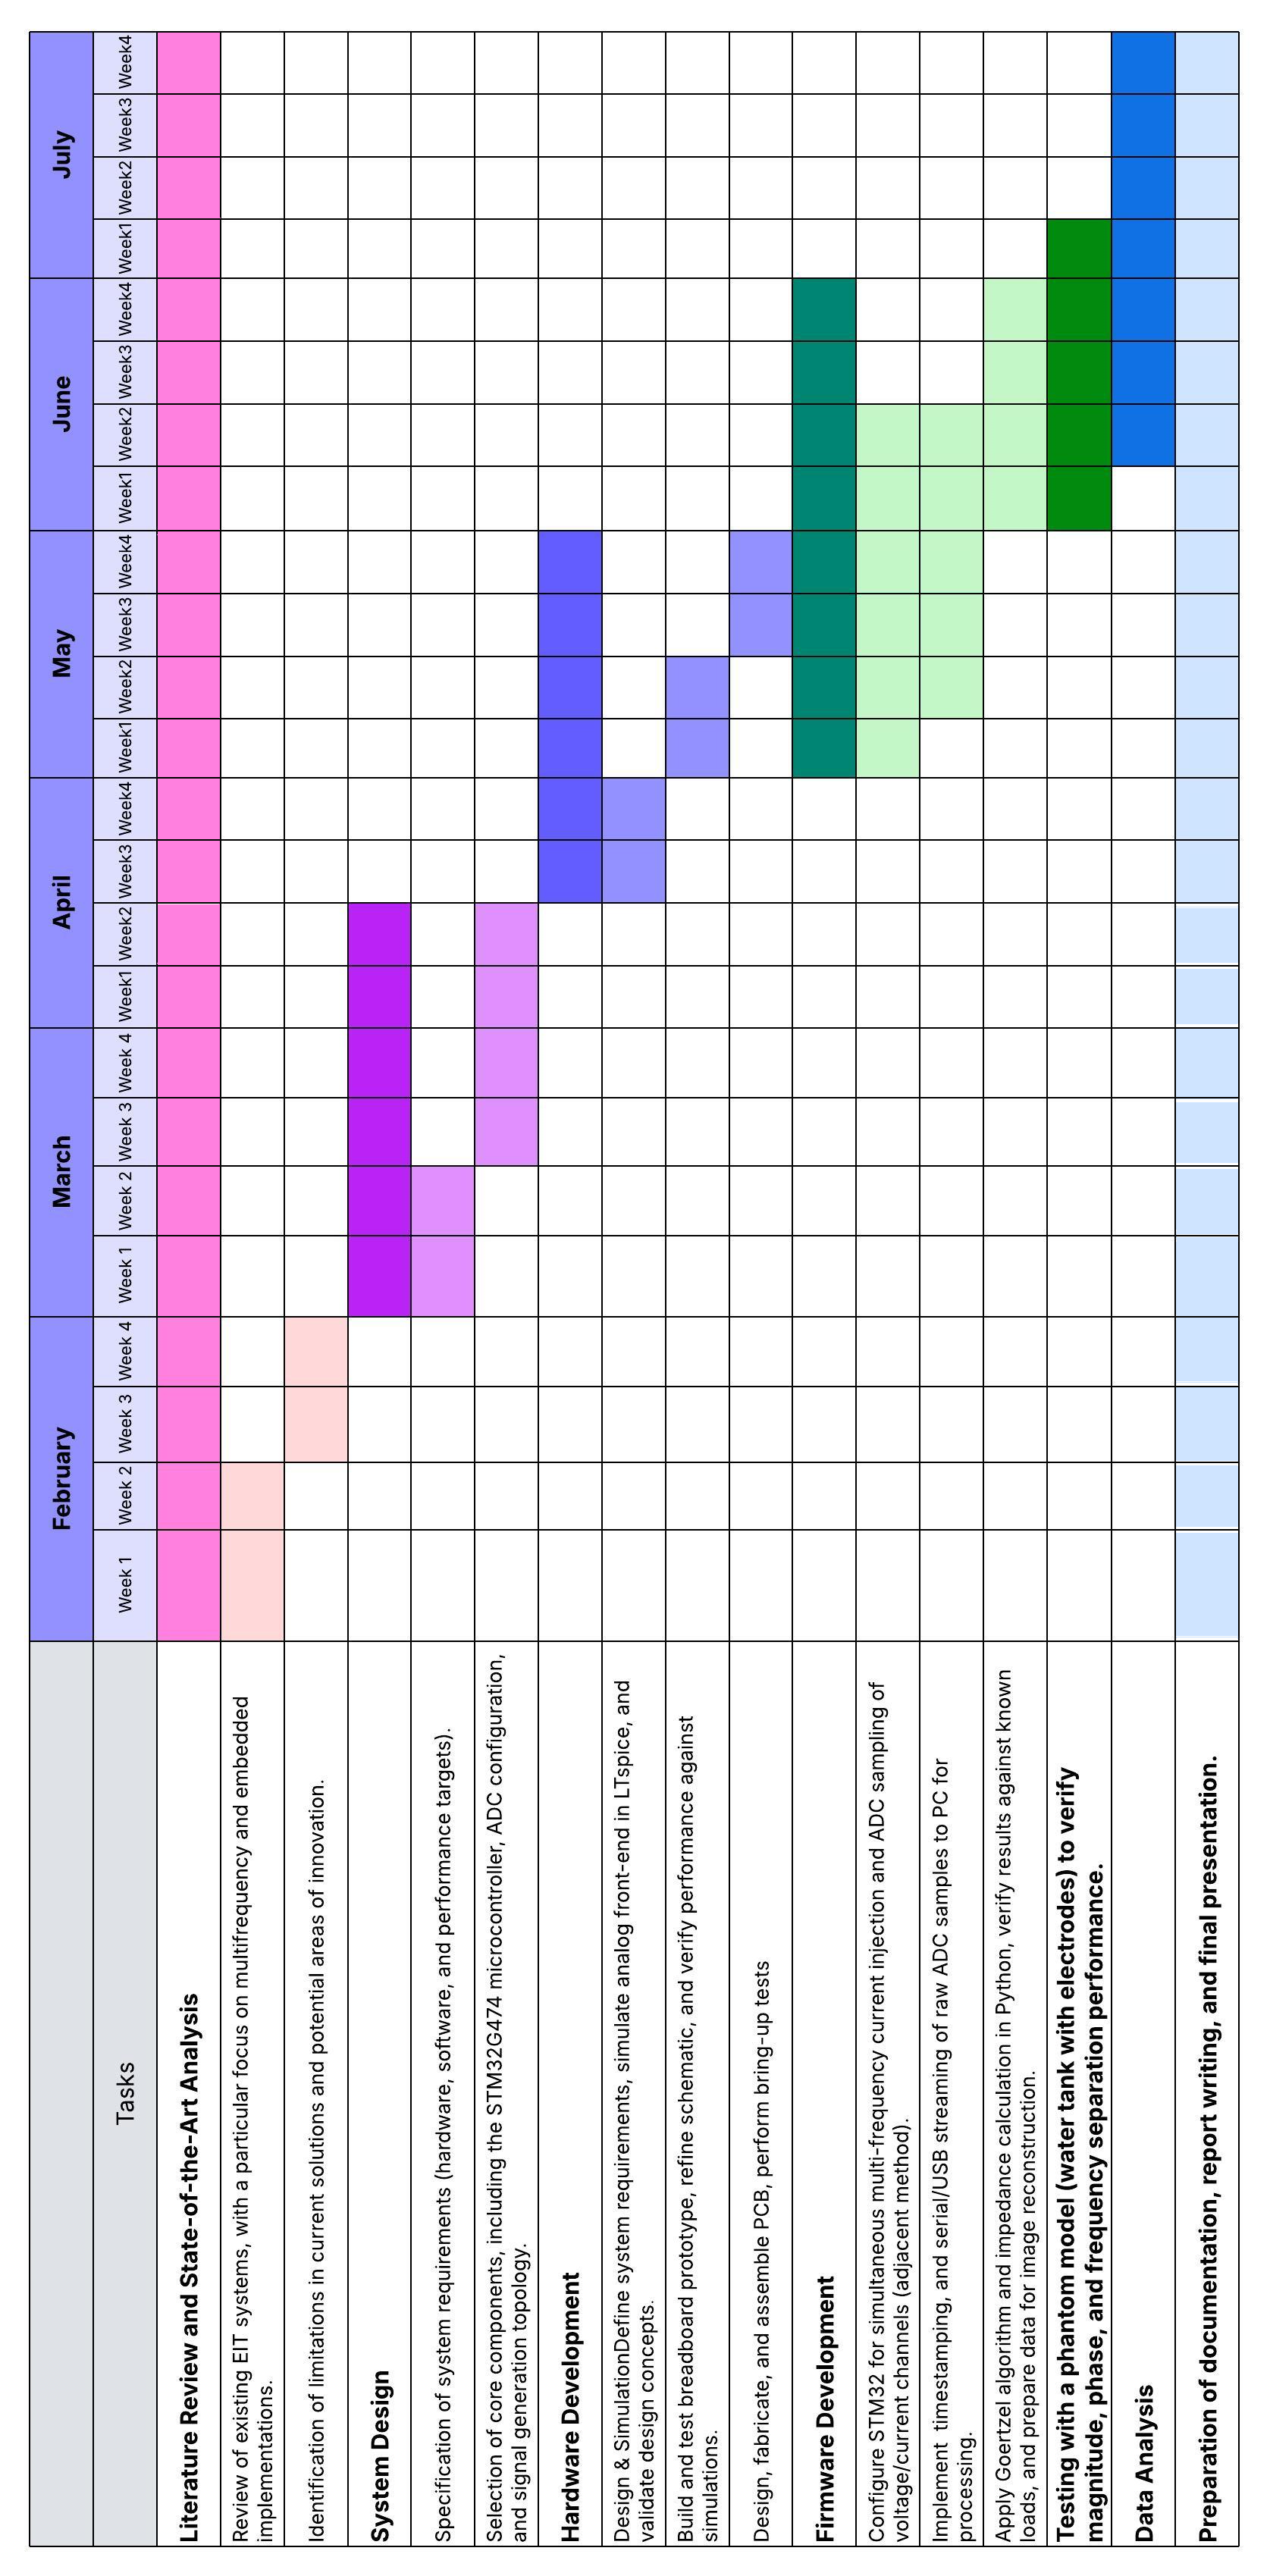
\includegraphics[width=0.7\textwidth]{imagess/gantt.png}
    \caption{Project work methodology and timeline (Gantt chart).}
    \label{fig:stability_lowfreq}
\end{figure}

\section{ Conclusion}
This chapter provided an overview of the host organization, structure, facilities, and international
associations to place the professional environment within which
the project was conducted. It also explained the background and motivation behind the work,
defined the problem statement, and set the project objectives. Finally, the adopted work
methodology and corresponding Gantt diagram were provided to display the formalized
procedure and scheduled plan for project completion. This forms the foundation of subsequent
chapters, which will record the technical design, development, and verification of the proposed
simultaneous multi-frequency Electrical Impedance
Tomography (EIT) system for biomedical purposes.

\chapter*{Chapter 2}
\markboth{Chapter 2 }{ EIT systems in biomedical applications and proposed contribution} %pour afficher l'entete
\addcontentsline{toc}{chapter}{II EIT systems in biomedical applications and proposed contribution}

\textbf {\Huge EIT systems in biomedical applications and proposed contribution} \\ 

\setcounter{chapter}{2}
\setcounter{section}{0}

%\end{chapter1}
\section{Introduction}
Electrical Impedance Tomography (EIT) is a non-invasive imaging technique that reconstructs the conductivity distribution in a body from small electrical currents introduced into the body and measured surface voltages. Due to the safety, portability, and low cost of EIT, it has gained increasing attention for biomedical applications, such as monitoring the lung, brain imaging, and cancer detection. This chapter overviews the fundamentals of EIT, reports recent advances in multi-frequency EIT systems, and discusses current limitations
and introduces our proposed method for better multi-frequency EIT performance.


\section{Fundamentals of EIT}
Electrical Impedance Tomography (EIT) is a tomographic method that reconstructs the
image of the internal electrical properties of a medium, typically biological tissue, from surface
electrical measurements. It relies on injecting small alternating currents into the body through
body surface electrodes and measuring the resultant voltages. The spatial distribution of
electrical conductivity and permittivity inside the body affects
these measurements, which can enable image reconstruction\cite{WikipediaEIT}
\subsection{Measurement protocols}
\begin{itemize}
\item
For Electrical Impedance Tomography (EIT), a ring of electrodes is
arranged evenly around the region to be investigated, e.g., the chest
or forearm. In our system, we used 16 circularly disposed electrodes.
To obtain data, a small, known alternating current (AC) is injected
between two selected electrodes—typically adjacent or opposite pairs. This injected current propagates through
the tissues, and the resulting voltage differences are sensed by the remainder of
electrodes. By successively varying the pair of electrodes used to inject the current and measure
the resulting voltages at other electrodes, we are able to get a full set of measurements
that sample the internal distribution of electrical impedance. These are acquired as
input for image reconstruction algorithms in order to produce conductivity maps of
the target tissue.
This technique allows us to study the electrical properties of the tissue, as different types of tissues affect current conduction in typical ways because of their individual conductivity and permittivity.




\item
The array of electrodes used for injecting current and for sensing voltage is called the measurement pattern. Different patterns control the sensitivity distribution, resolution, and the depth of the reconstructed image\cite{MDPI2021}:
\begin{itemize}
\item Adjacent pattern: Current is injected through a pair of neighboring electrodes, and voltage measurements are collected from the remaining electrode
pairs. This approach is widely used due to its simplicity and ability to provide good
spatial sensitivity near the boundary.
\item Opposite pattern: Current is passed between opposite electrodes
(e.g., E1–E9 in a 16-electrode system), improving sensitivity in the central region.
\item Skip patterns: Current is passed between electrodes skipped by one or more intermediate electrodes. As an example, skip-1 uses E1–E3, skip-2 uses E1–E4, etc. These patterns offer a trade-off between central and boundary sensitivity.\cite{Adler2016}\\
In this project, we selected the adjacent injection to maximize boundary sensitivity .
\end{itemize}

In this work, the adjacent injection protocol was chosen to maximize boundary sensitivity, as illustrated in Figure~\ref{fig:enter-label}.
\begin{figure}[H]
    \centering
    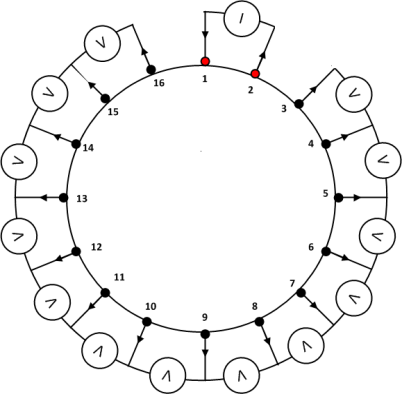
\includegraphics[width=0.4\linewidth]{imagess/AAA.png}
    \caption{EIT adjacent injection protocol using 16 electrodes.\cite{Angelucci2021}}
    \label{fig:enter-label}
\end{figure}
\end{itemize}
\subsection{Mathematical formulation}
After defining the measurement protocols, we now explore the mathematical challenges inherent in reconstructing conductivity images from voltage measurements.\\
Once voltage and current measurements have been collected from different current injection patterns, the next task in EIT is the reconstruction of the internal conductivity structure of the target region. The process is called solving the inverse problem.
In EIT, the forward problem is well-defined: with a known conductivity dist-
tribution, one can calculate the voltages on electrodes using Maxwell's equations

The inverse problem is the reverse: solving for conductivity distribution from known voltages.
The inverse problem in EIT is inherently:
\begin{itemize}
    \item \textbf{Nonlinear} : Conductivity and measured voltages are nonlinearly related.
    \item \textbf{Ill-posed} : Small measurement noise can create large errors in the reconstructed
image; multiple distributions of conductivity may fit the same voltage data.
    \item \textbf{Underdetermined} :  the unknowns (internal values of conductivity) are typically much larger than the number of measurements available.
\end{itemize}

The relationship can be expressed as \cite{Seo2019}:
\begin{equation}
V = F(\sigma) + \varepsilon
\label{eq:forward_model}
\end{equation}
where:
\begin{itemize}
    \item $V$ = vector of measured voltages
    \item $\sigma$ = conductivity distribution to be estimated
    \item $F$ = nonlinear forward model
    \item $\varepsilon$ = measurement noise
\end{itemize}
Figure~\ref{fig:enter-label} illustrates a schematic representation of the Electrical Impedance Tomography (EIT) process, showing how current is injected, boundary voltages are measured and then the image is reconstructed.


\begin{figure}[H]
    \centering
    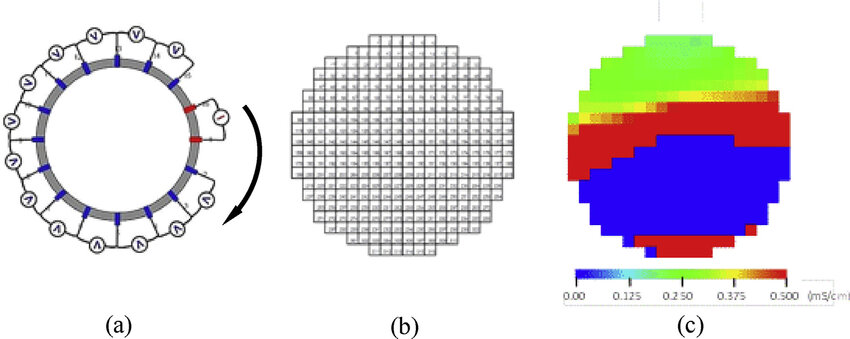
\includegraphics[width=0.8\linewidth]{imagess/Schematics-showing-a-the-adjacent-current-injection-pattern-for-a-circular-16-electrode.png}
    \caption{Schematic representation of the EIT process.\cite{Hou2016}}
    \label{fig:enter-label}
\end{figure}


\section{Frequency-dependent impedance properties of biological tissues}
Biological tissues are frequency dependent in their impedance properties, due in large part to cell membranes, intracellular and extracellular fluids, and tissue composition. At low frequencies, current travels mostly through the extracellular space because cell membranes act as capacitors, blocking direct current access into the cells. As frequency is increased, the membrane capacitive reactance decreases, and current can enter the intracellular space.

This property is exploited in \textit{multi-frequency EIT} (MFEIT) to provide improved tissue characterization and discrimination. By having EIT data at multiple frequencies, it is possible to discriminate between tissues or to identify physiological changes that would not be visible with single-frequency data.

This frequency-dependent response is particularly useful for biomedical applications when detecting pathological changes such as edema, ischemia, or tumor development since such conditions often alter the dielectric properties of tissues at certain frequency \cite{Bera2017}.
\\The figure 2.7 illustrates how the electrical impedance of biological tissues changes with frequency, showcasing the characteristic frequency-dependent behavior exploited in multi-frequency EIT.
\begin{figure}[H]
    \centering
    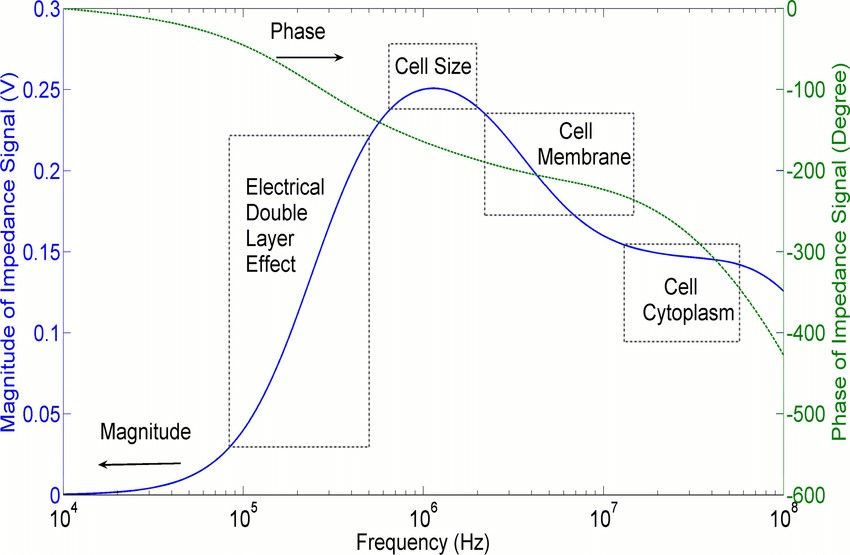
\includegraphics[width=0.8\linewidth]{imagess/8dhl6ptn.png}
    \caption{Measured tissue impedance as a function of frequency\cite{Sun2008}}
    \label{fig:enter-label}
\end{figure}

\end{itemize}
\section{Multi-frequency EIT methods}
In order to evaluate the progress and challenges of multi-frequency EIT, it is essential to review and compare the main systems proposed in the literature. Several implementations have been reported with differences in electrode configurations, excitation strategies, frequency ranges, and data acquisition methods. A comparative analysis highlights the advantages and trade-offs of these approaches, providing a reference against which the proposed system can be positioned.
\subsection{Benchmarking}
Multi-frequency Electrical Impedance Tomography (MFEIT) extends the capabilities of conventional single-frequency EIT by acquiring data over a range of frequencies. 
This approach leverages the frequency-dependent electrical properties of biological tissues, enabling improved differentiation between tissue types, enhanced image reconstruction, and the extraction of additional physiological information. 

\begin{table}[H]
\centering
\caption{ Multi-frequency EIT systems }
\resizebox{\textwidth}{!}{%
\begin{tabular}{|m{1cm}|m{2cm}|m{3.5cm}|m{3.5cm}|m{2.5cm}|m{2.5cm}|m{2.5cm}|m{3cm}|m{3.5cm}|}
\hline
\textbf{Ref} & \textbf{Electrodes} & \textbf{Frequency range \& number} & \textbf{Data type} & \textbf{ADC resolution} & \textbf{MCU} & \textbf{Excitation type} & \textbf{Acquisition time} & \textbf{Application} \\ \hline
\cite{Klosowski2025} & 32 & 100 kHz, 50 kHz, 10 kHz, 3 freqs & Resistive, Reactive & – & Dual-core ARM Cortex-A9 & Single sine wave & – & Industrial \\ \hline
\cite{LiWang2025} & – & 10–100 kHz & Magnitude, Phase & – & – & Sequential MF & 10–100 fps & Medical, Industrial, Geo \\ \hline
\cite{Chen2021} & 16 & 10–100 kHz, 5 freqs & Voltage & – & – & sequential MF & – & Biomedical \\ \hline
\cite{Yang2022} & 16 & 100 kHz–1 MHz & Amplitude, Phase & 12-bit & DSP TMS320 F28335 & Sequential MF & 208 voltages/cycle & Biomedical, Industrial, Agricultural \\ \hline
\cite{Zhu2024} & 12 & 10 kHz–1 MHz, 3 freqs & Impedance & 16-bit & STM32F103 & Sequential MF & 15 fps & Biomedical \\ \hline
\cite{Sensors2019} & 16 & 60–960 kHz, 2 freqs & I/Q Demodulation & 14-bit & Virtex-6 FPGA & Simultaneous MF & 32.8–131 fps & Lung, Cardiac, Perfusion monitoring \\ \hline
\end{tabular}%
}

\label{tab:eit-comparison}
\end{table}


Table 2.1 summarizes recent multi-frequency EIT implementations across various applications, highlighting differences in electrode configurations, frequency ranges, excitation types, ADC resolutions, and acquisition methods. While these systems demonstrate progress toward multi-frequency impedance imaging, the analysis reveals persistent trade-offs between acquisition speed, frequency coverage, measurement precision, and application-specific requirements. Notably, the majority of biomedical-focused systems rely on sequential frequency excitation, limiting temporal resolution and robustness in dynamic environments. Additionally, ADC resolution and simultaneous acquisition capabilities vary widely, indicating significant room for improvement to meet the stringent demands of real-time clinical monitoring.

\subsection{Limitations }
In Electrical Impedance Tomography (EIT), conventional systems often operate at a single frequency (monofrequency). While simple and fast, monofrequency measurements cannot capture frequency-dependent tissue properties, such as the difference between extracellular and intracellular conductivity. This limits the ability to distinguish different tissue types or monitor complex physiological processes.

To address this, many systems use sequential multi-frequency excitation, where currents are applied one frequency at a time and the resulting voltages are measured before moving to the next frequency ([12], [13], [15], [21]; see Table 2.1). Sequential systems are relatively easy to implement, but they have several limitations. First, the overall acquisition time increases proportionally with the number of frequencies, which can be a problem in fast-changing biological conditions. Second, motion artifacts may occur between frequencies: physiological movements, such as heartbeats, breathing, or patient motion, can alter the measured voltages from one frequency to the next. These temporal inconsistencies create errors and distortions in the reconstructed impedance images, reducing spatial accuracy and reliability.

Some advanced systems, such as [26], implement simultaneous acquisition but are limited to only two discrete frequencies. While better than sequential methods, this still restricts the frequency range and reduces the ability to exploit the full spectral information of biological tissues.

The main challenge in multi-frequency EIT is therefore to develop systems that can excite and measure multiple frequencies at the same time. Simultaneous multi-frequency EIT reduces overall measurement time, eliminates motion artifacts between frequencies, and improves imaging accuracy and reliability. This is essential for dynamic, real-time biomedical applications, such as monitoring muscle activity, lung function, or other rapid physiological processes.

\section{Proposed approach for enhancement of multi- frequency EIT}

To overcome the limitations of existing multi-frequency EIT systems, this work proposes a simultaneous multi-frequency excitation and measurement strategy designed to improve temporal resolution and enhance diagnostic precision. Unlike traditional sequential frequency sweeps, the simultaneous approach enables real-time acquisition of frequency-dependent tissue information, thereby minimizing motion artifacts and better capturing rapid physiological changes.  

The proposed system architecture is organized around several key building blocks. A dedicated current source (VCCS) generates stable multi-frequency excitation signals that are applied to a set of boundary electrodes through multiplexers and demultiplexers. The selection of electrode pairs for current injection and voltage measurement is controlled dynamically, enabling flexible measurement patterns. The STM32G474 microcontroller forms the core of the system, integrating a high-speed DAC for excitation signal generation and high-resolution ADCs for voltage acquisition. Signal conditioning modules are employed to ensure measurement integrity by filtering noise, stabilizing signals, and matching impedance before digitization. The acquired signals are then processed in real time to separate frequency components, compute impedance values, and prepare the data for higher-level analysis. This integrated architecture makes the system compact, efficient, and suitable for portable biomedical applications.  


A central innovation in the proposed approach lies in the excitation strategy. Instead of using simple sinusoidal signals, a specially optimized multisine stimulus is employed. The frequency components of this multisine are carefully selected using an optimization algorithm that balances two criteria: (i) maximizing spectral coverage across the frequencies of interest, and (ii) minimizing interference and harmonic distortion between components. The optimization process ensures that injected signals remain orthogonal and well-separated, enabling accurate frequency-domain analysis even under simultaneous operation. Compared to sequential frequency sweeps, this optimized multisine excitation significantly reduces measurement time while increasing robustness against motion artifacts, thus paving the way for precise and real-time biomedical imaging.  

The subsequent chapters present the detailed system design and implementation. Chapter~3 elaborates on the architecture, hardware realization, and signal conditioning techniques, while Chapter~4 discusses the signal processing methods and validates the proposed approach through experimental results.

\section{Conclusion}

In this chapter, a comprehensive description of existing multi-frequency Electrical Impedance Tomography systems was presented, indicating their current shortcomings in terms of temporal resolution, measurement accuracy, and susceptibility to motion artifacts. To address these problems, a novel idea of simultaneous multi-frequency excitation and high-resolution data acquisition using the 16-bit ADC of STM32G4 microcontroller was proposed. The use of an optimized multisine excitation signal further develops the potential of the system since it enables simultaneous frequency measurements in an efficient and accurate way.
This proposed approach offers a sound foundation for higher fidelity images and
biomedical real-time processing. The design and implementation details will be covered
in the following chapter.


\chapter*{chapter 3}
\markboth{Chapter 3 }{ Hardware and software system design } %pour afficher l'entete
 \addcontentsline{toc}{chapter}{III   Hardware and software system design }

\textbf{\Huge Hardware and software system design} 

\setcounter{chapter}{3}
\setcounter{section}{0}


\section{Introduction}
This chapter describes the design and implementation of the proposed simultaneous multi-
frequency EIT system. The process of development includes signal specification, hardware
design, PCB development, and firmware implementation on the STM32G4 platform. The
design should possess a high temporal resolution and accurate impedance measurements
through optimized multisine excitation and high-resolution 16-bit ADC sampling.
\section{Excitation signal specification}
In the proposed system, the excitation waveform is a \textit{multisine} signal generated by superimposing sinusoidal components at carefully selected frequencies. The selection of frequency values, frequency spacing, and amplitudes directly influences measurement precision, spectral range, and ability to follow impedance variations over a large bandwidth.
To verify performance, two configurations were employed and tested:
\begin{itemize}
    \item \textbf{Two-frequency multisine:} Reduced spectral coverage, used primarily for first-stage validation of the acquisition chain.
\item \textbf{Five-frequency multisine:} Sufficient coverage with less complexity, offering a compromise
towards the speed of measurement and spectral resolution.
\end{itemize}
For every configuration, the frequencies were selected in order to minimize harmonic overlap and intermodulation distortion, subject to the IEC 60601 amplitude limit requirements for biomedical safety.


\noindent
The generation of the excitation signal follows the algorithm illustrated in Figure~\ref{fig:multisine_algorithm}, implemented using a dedicated Python script.

\begin{figure}[H]
    \centering
    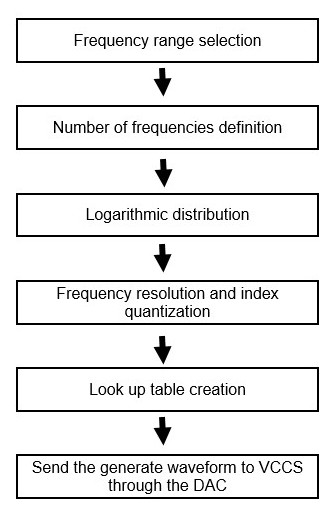
\includegraphics[width=0.4\linewidth]{imagess/Slide2.jpg}
    \caption{Flowchart of the multisine excitation signal generation process}
    \label{fig:multisine_algorithm}
\end{figure}

\subsection{Mathematical formulation of the excitation signal generation algorithm}
The procedure for generating the excitation signal consists of the following main steps:

\paragraph{Step 1: Frequency range definition}\\
The minimum and maximum frequencies are defined as: f_{\min}, \; f_{\max}


\paragraph{Step 2: Logarithmic frequency spacing}\\
For a total of \( N_{\text{freq}} \) frequencies, the logarithmic distribution is computed as:
\begin{equation}
f_k = f_{\min} \cdot \left( \frac{f_{\max}}{f_{\min}} \right)^{\frac{k}{N_{\text{freq}}-1}}, \quad k = 0, 1, \dots, N_{\text{freq}}-1
\label{eq:log_spacing}
\end{equation}

\paragraph{Step 3: Frequency quantization to FFT bins}\\
Considering a sampling frequency \( f_s \) and FFT length \( N_{\text{FFT}} \), the frequency resolution is:
\begin{equation}
\Delta f = \frac{f_s}{N_{\text{FFT}}}
\label{eq:delta_f}
\end{equation}
Each frequency is quantized to the nearest FFT bin:\\
\begin{equation}
f_k^{(q)} = \text{round}\left( \frac{f_k}{\Delta f} \right) \cdot \Delta f
\label{eq:quantization}
\end{equation}

\paragraph{Step 4: Multisine signal synthesis}\\
The discrete-time multisine signal is:
\begin{equation}
x[n] = \sum_{k=0}^{N_{\text{freq}}-1} A_k \cdot \sin\left( 2\pi \frac{f_k^{(q)}}{f_s} n + \phi_k \right)
\label{eq:multisine}
\end{equation}
where \( A_k \) is the amplitude of the \( k \)-th component and \( \phi_k \) is a random initial phase.

\paragraph{Step 5: Amplitude normalization and DAC mapping}\\
The signal is normalized to the DAC range \([0, 2^{N_{\text{bits}}} - 1]\):
\begin{equation}
x_{\text{DAC}}[n] = \left\lfloor \frac{x[n]}{\max |x[n]|} \cdot \left(2^{N_{\text{bits}}-1} - 1\right) + 2^{N_{\text{bits}}-1} \right\rfloor
\label{eq:dac_mapping}
\end{equation}
For the 12-bit DAC used in this work: \( N_{\text{bits}} = 12 \).


\paragraph{Step 6: LUT generation}\\
The final samples are stored in both CSV format and C header files for direct microcontroller integration.

\subsection{Component selection and justification}
The following table summarizes the key hardware components selected for the system, along with a brief description and justification for their inclusion.

\begin{table}[H]
\centering
\caption{Hardware component selection and justification}
\begin{tabular}{|p{4cm}|p{5cm}|p{7cm}|}
\hline
\textbf{Requirement} & \textbf{Selected component} & \textbf{Justification} \\
\hline
Low-noise precision amplification & ADA4610-2ARZ (Analog Devices) & Offers ultra-low input bias current (1 pA), low offset (50 $\mu$V), and low noise density (3 nV/$\sqrt{\text{Hz}}$), which is critical for microvolt-level EIT boundary voltage measurements\cite{ada4610}.\\
\hline
Scalable electrode switching & CD74HC4067SM96(Texas Instruments) & 16-channel analog multiplexer (16:1) with low ON resistance ($\sim$70 $\Omega$). Provides wide analog bandwidth ($\sim$89 MHz, $-3$ dB) suitable for the maximum excitation frequency of 2.5 MHz ($f_{\text{MUX}} \geq 2 \cdot N \cdot f_{\text{exc,max}}$), This ensures minimal distortion and correct per-channel sampling\cite{cd74hc4067}.\\

\hline
\end{tabular}
\end{table}
\begin{table}[H]
\centering
\begin{tabular}{|p{4cm}|p{5cm}|p{7cm}|}
\hline
\textbf{Requirement} & \textbf{Selected component} & \textbf{Justification} \\
\hline
Signal generation, acquisition, and control & STM32G474RE (STMicroelectronics) & Integrated high-speed ADC (up to 4 MSPS, 12-bit). Supports DMA for efficient data acquisition and multiple GPIOs for multiplexer control. Chosen due to its superior analog performance, processing capability, and robust development ecosystem (CubeMX, HAL, STM32 IDE)\cite{stm32g474re}. \\
\hline
Stable current excitation & Modified dual Howland VCCS with AD8021 op-amp & Provides stable AC currents (≤0.4 mA peak) across 50 kHz–1 MHz and 100 Ω–18 kΩ loads. Low-power design (5 V supply, 210 mW) ensures compliance with IEC-60601 safety standards. Supports multisine excitation, maintaining stability, enhancing accuracy and portability for wearable EIT applications\cite{ouni2024}.\\
\hline
\end{tabular}
\end{table}


\section{EIT circuit simulation on LTspice}
\label{sec:eit-ltspice}

Before investing in hardware, the EIT acquisition chain was verified with LTspice using
a controlled "known-resistor" device-under-test (DUT) rather than biological tissue or
the salt tank. This process validates the path of excitation, the analog front-end, and the
impedance extraction algorithm (voltage and current measurement), with the aim that
computed resistance is equivalent to the DUT component across the operating bandwidth.The full LTspice schematic of the simulated acquisition circuit is shown in Figure 3.9.

\begin{figure}[H]
    \centering
    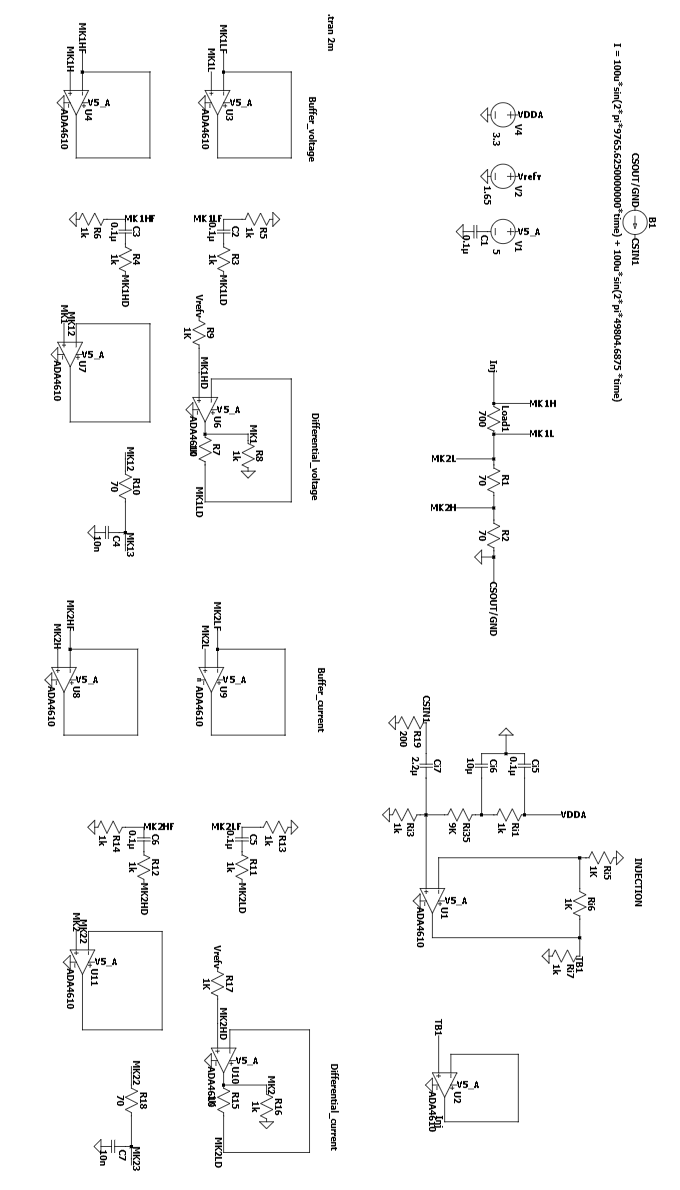
\includegraphics[width=0.8\textwidth]{imagess/LTspice_circuit.png}
    \caption{LTspice schematic of the simulated EIT acquisition circuit.}
    \label{fig:ltspice}
\end{figure}


\subsection{Excitation signal conditioning:}  
As shown in figure 3.10 the input excitation current $I_{\text{CSIN1}}$ is first converted into a small voltage by the resistor $R_{19}=200~\Omega$, yielding an AC voltage of approximately $100~\text{mV}$ peak for a $500~\mu\text{A}$ input. 
This AC signal is then coupled through $C_7=2.2~\mu\text{F}$, which blocks any DC component.\\
In this project, the EIT system is used to reconstruct the conductivity distribution of certain biomedical tissues, and its performance will be validated
with a water tank experiment. Since the conductivity profiles of the DUTs
are very different, a special excitation signal adjustment circuit is required.
The purpose of this circuit is to maintain the excitation signal within the
range so that the resulting output falls within the compatibility range of the amplifier input window and to scale both the DC
and AC components of the signal accordingly.
A resistive divider biases this AC signal to a suitable DC level. 
The resistors are defined as:  
\[
R_{i35} = 9~\text{k}\Omega, \quad R_{i1} = R_{i3} = 1~\text{k}\Omega
\]
With a supply voltage $V_{DDA} = 3.3~\text{V}$, the DC bias voltage at the junction of $R_{i1}$, $R_{i3}$ and $R_{i35}$ is:

\begin{equation}
    V_{DC} = V_{DDA} \cdot \frac{R_{i1}}{R_{i3} + R_{i35}}
\end{equation}

Substituting the values:  

\[
V_{DC} = 3.3 \cdot \frac{1~\text{k}\Omega}{1~\text{k}\Omega + 9~\text{k}\Omega} 
= 3.3 \cdot \frac{1}{10} 
= 0.33~\text{V}
\]  

This means the excitation signal is shifted to approximately $0.33~\text{V}$ DC. 
The AC amplitude is then adjusted by the amplification stage.

As shown in the figure, the op-amp (ADA4610) is configured as a non-inverting amplifier with the feedback resistors:  
\[
R_{i5} = R_{i6} = 1~\text{k}\Omega
\]

The gain is given by:  
\begin{equation}
G_1 = 1 + \frac{R_{i5}}{R_{i6}}
\end{equation}

Thus, the amplification factor is $G_1 = 2$, doubling the AC component while preserving the DC bias. 
Finally, the signal is passed to a unity-gain buffer stage, which provides the necessary drive capability for safe electrode injection without loading the adjustment circuit.
The buffer gain is ideally:
    G_{\mathrm{buf}} \approx 1.

\subsection{AC coupling and biasing (per channel)}
The boundary electrode voltages $V_{\text{in1}}$ and $V_{\text{in2}}$ are first buffered
by unity-gain amplifiers (ADA4610) to provide high input impedance and prevent
loading of the electrodes. The buffered signals are then AC-coupled through
capacitors $C_{2}$ and $C_{3}$.

Each capacitor, together with its associated resistor pair, forms a first-order
high-pass filter: $(C_{2},R_{5},R_{3})$ for the upper channel and
$(C_{3},R_{4},R_{6})$ for the lower channel. These filters block DC electrode
offsets and pass only the AC components of interest. The general transfer
function of each filter is

\begin{equation}
  H_{\mathrm{HP}}(j\omega) = \frac{j\omega R_{\mathrm{eq}} C}{1 + j\omega R_{\mathrm{eq}} C},
  \qquad f_c = \frac{1}{2\pi R_{\mathrm{eq}} C},
\end{equation}

where $R_{\mathrm{eq}}$ is the effective resistance seen by the capacitor. For
$R=1~\text{k}\Omega$ and $C=0.1~\mu\text{F}$, we obtain

\[
f_c = \frac{1}{2 \pi \cdot 1~\text{k}\Omega \cdot 0.1~\mu\text{F}}
     \approx 1.59~\text{kHz}.
\]

Because both channels use identical RC values, the two filters are matched in
gain and phase, which ensures accurate differential subtraction in the next
stage.



  
\subsection{Differential boundary voltage measurement}

The filtered signals are then applied to a differential amplifier with matched resistor ratios (feedback resistor $R_7$ and input resistor $R_9$), the transfer function can be written as

\begin{equation}
V_{\mathrm{out}} \;=\; \frac{R_7}{R_9}\,\bigl(V_{\text{in2}} + V_{\mathrm{ref}} - V_{\text{in1}}\bigr),
\end{equation}

where $V_{\text{in2}}$ and $V_{\text{in1}}$ are the two measurement nodes of the DUT and $V_{\mathrm{ref}}$ is a DC offset applied to shift the amplifier output into the ADC input range.

With $R_7 = R_9 = 1~\text{k}\Omega$ (matched resistors), the differential gain is unity:

\begin{equation}
G_{\mathrm{diff}} \;=\; \frac{R_7}{R_9} \;=\; 1,
\end{equation}

so the expression simplifies to
\begin{equation}
V_{\mathrm{out}} \;=\; V_{\text{in2}} - V_{\text{in1}} + V_{\mathrm{ref}}.
\end{equation}

Here, $V_{\mathrm{ref}} = 1.65\ \text{V}$ is chosen because it is the midpoint of the ADC input range (3.3~V). This centers the amplifier output around mid-scale, allowing small bipolar differential voltages $(V_{\text{in2}}-V_{\text{in1}})$ to be measured without saturating the ADC:

\begin{equation}
V_{\mathrm{out}} \;=\; V_{\text{in2}} - V_{\text{in1}} + 1.65\ \text{V}.
\end{equation}
Figure~\ref{fig:eit_injection1} illustrates the excitation adjustment stage along with the differential boundary voltage measurement circuit, which ensures that the injected signal remains within the ADC input range while accurately capturing the small voltage differences across the DUT
\begin{figure}[H]
    \centering
    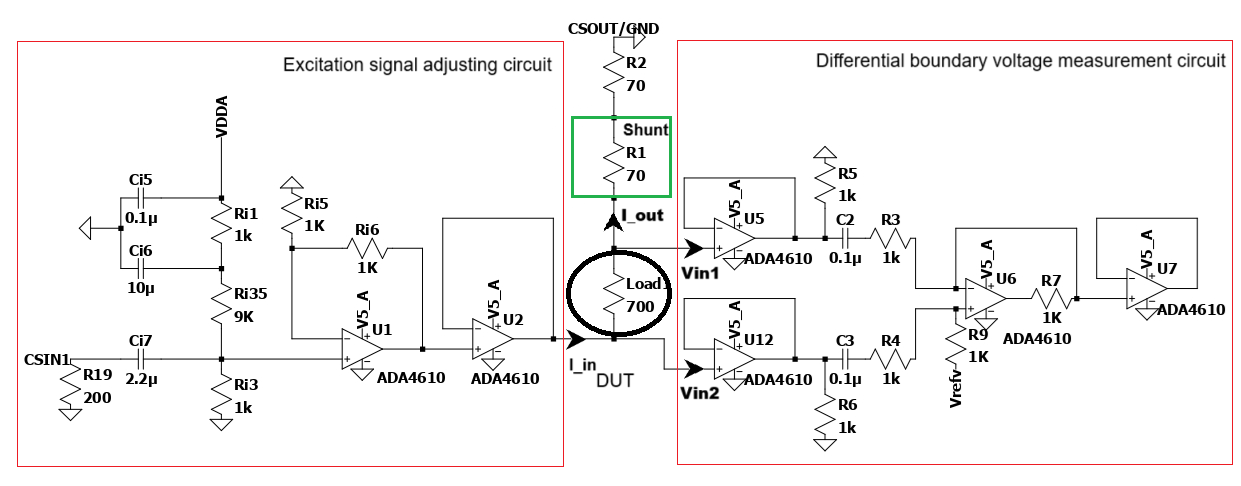
\includegraphics[width=1\linewidth]{imagess/injection_differentiaal.png}
    \caption{Excitation signal adjusting and differential boundary voltage measurement circuit}
    \label{fig:eit_injection1}
\end{figure}

\subsection{Differential current measurement circuit}  
In addition to boundary voltage acquisition, the injected current across the DUT must also be properly measured for impedance extraction. The same signal conditioning principle is applied:
first, the minor voltage drop on the precision shunt resistor ($R_{\text{shunt}}$) is buffered to provide high input impedance, and then similar high-pass filters are also used to guarantee that no DC component is delivered to the tissue. Then a differential amplifier stage suppresses common-mode
noise and extracts the actual shunt voltage.
For the traditional difference amplifier configuration with matched resistors (feedback
resistor $R_13$ and input resistor $R_17$), the transfer function is represented by



\begin{equation}
V_{\mathrm{out,\,I}} \;=\; \frac{R_{13}}{R_{17}}\,\bigl(V_{+} - V_{-} + V_{\mathrm{ref}}\bigr)
\end{equation}


where $V_{+}$ and $V_{-}$ are the voltages across the shunt resistor, and $V_{\mathrm{ref}}$ is the same DC offset (1.65~V) used to center the output within the ADC input range.

With $R_13 = R_17 = 1~\text{k}\Omega$, the differential gain is unity:

\begin{equation}
G_{\mathrm{diff}} \;=\; \frac{R_13}{R_17} \;=\; 1,
\end{equation}

and the expression simplifies to

\begin{equation}
V_{\mathrm{out,\,I}} \;=\; V_{+} - V_{-} + V_{\mathrm{ref}}.
\end{equation}

Since $V_{+}-V_{-}$ corresponds to the voltage drop across $R_{\text{shunt}}$, the output directly reflects the instantaneous current, shifted by the reference offset:

\begin{equation}
I_{\text{DUT}} \;=\; \frac{V_{+} - V_{-}}{R_{\text{shunt}}}, \qquad
V_{\mathrm{out,\,I}} \;=\; I_{\text{DUT}} \cdot R_{\text{shunt}} + V_{\mathrm{ref}}.
\end{equation}

This configuration ensures that both voltage and current measurement channels share the same architecture (buffering stage followed by differential amplification), providing high common-mode rejection, symmetry in signal processing, and robust performance in noisy environments.
  
Figure~\ref{fig:current_measurement_circuit} shows the practical realization of the current measurement circuit. The buffered differential amplifier processes the shunt voltage and outputs a mid-scale referenced signal suitable for digitization by the ADC. The layout mirrors the voltage measurement circuit, thereby simplifying design complexity and improving overall noise immunity.

\begin{figure}[H]
    \centering
    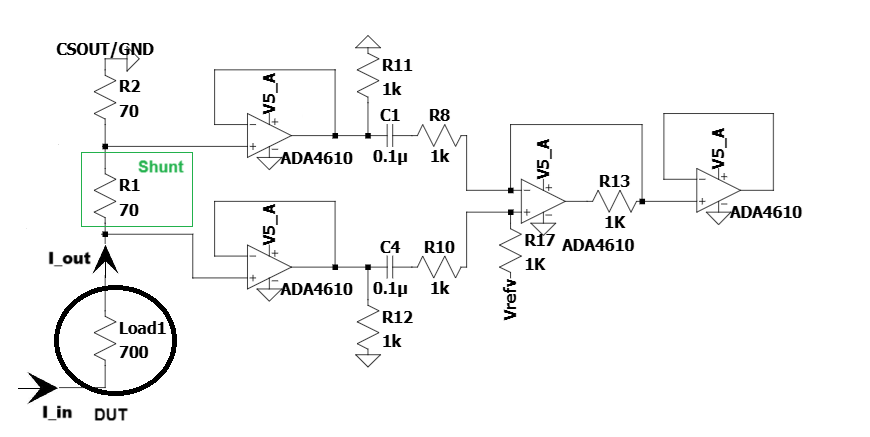
\includegraphics[width=1\textwidth]{imagess/Untitled (Recovered).png}
    \caption{Schematic of the current measurement circuit based on buffering and differential amplification.}
    \label{fig:current_measurement_circuit}
\end{figure}

   
\end{enumerate}

\subsection{Excitation and simulation settings}

\begin{itemise}
    \item \textbf{Load modeling:}  
Instead of the actual water tank with a metallic inclusion, the Device Under Test (DUT) 
was represented by a known resistor $R_{\text{load}}$. This substitution enables the 
verification of whether the simulation can recover the expected resistance value from 
the measured voltage and current. For example, when $R_{\text{load}} = 1~k\Omega$, the 
simulation should return a measured resistance close to $1~k\Omega$.

\item \textbf{Shunt resistor:}  
A shunt resistor $R_{\text{shunt}}$ of $70~\Omega$ was placed in series with the DUT 
to allow current measurement. The voltage drop across the shunt is processed by the 
current-differential amplifier in the real system. The choice of $70~\Omega$ represents 
a compromise: it is large enough to generate a measurable voltage drop for the amplifier 
while remaining small enough to avoid significantly perturbing the injected current.  
The instantaneous current through the DUT is thus obtained as : 

\begin{equation}
I_{\text{measured}}(t) = \frac{V_{\text{shunt}}(t)}{R_{\text{shunt}}}.
\end{equation}
\end{itemise}
The simulation was run in transient mode over a duration of $2~ms$, sufficient to capture 
multiple cycles of both excitation frequencies. 

Finally, the resistance was computed using the ratio of the measured voltage to the 
calculated current:
\begin{equation}
R_{\text{calculated}} = \frac{V_{\text{DUT}}}{I_{\text{measured}}}.
\end{equation}

\subsection{Results visualization and resistance calculation.}  



\paragraph{(A) Time-Domain Verification Using Single-Frequency Excitation}
The figure~\ref{fig:eit_injection} illustrates the injected current after passing through the injection circuit. A current source with the expression :
\begin{equation}
I(t) = 100~\mu A \cdot \sin(2\pi \cdot 9765.625 \cdot t) 
\end{equation}
(single-frequency) was used, and the plot shows the resulting waveform of the injected current.
\begin{figure}[H]
    \centering
    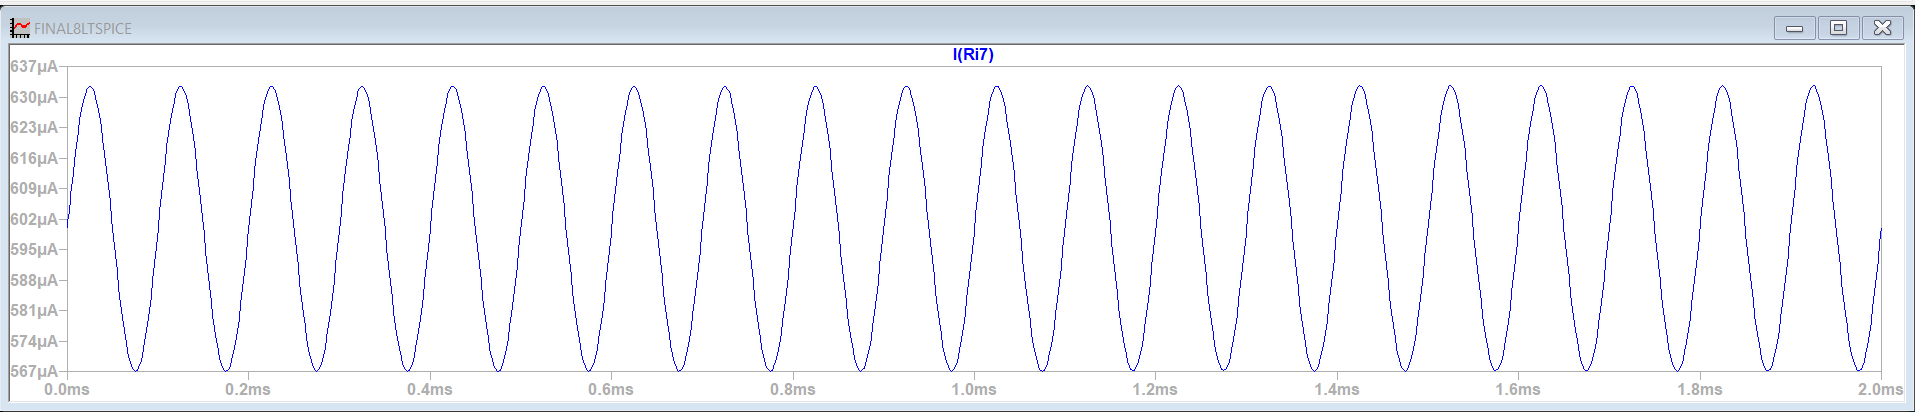
\includegraphics[width=1\linewidth]{imagess/Inj.png}
    \caption{Measured DUT current waveform obtained via shunt calculation.}
    \label{fig:eit_injection}
\end{figure}


\noindent Figures~\ref{fig:eit_voltage} and~\ref{fig:eit_current} present the measured 
voltage and current waveforms respectively. These plots confirm that both signals follow 
the expected sinusoidal behavior dictated by the sinewave excitation source.

\begin{figure}[H]
    \centering
    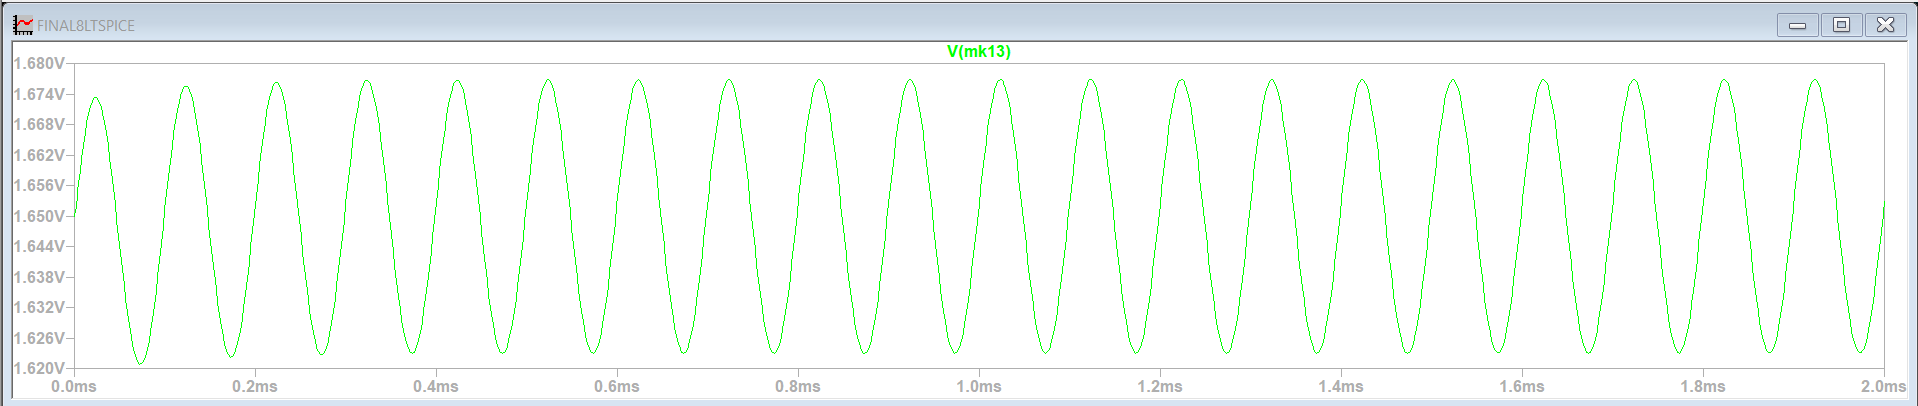
\includegraphics[width=1\linewidth]{imagess/voltage_700_70.png}
    \caption{Measured DUT voltage waveform.}
    \label{fig:eit_voltage}
\end{figure}

\begin{figure}[H]
    \centering
    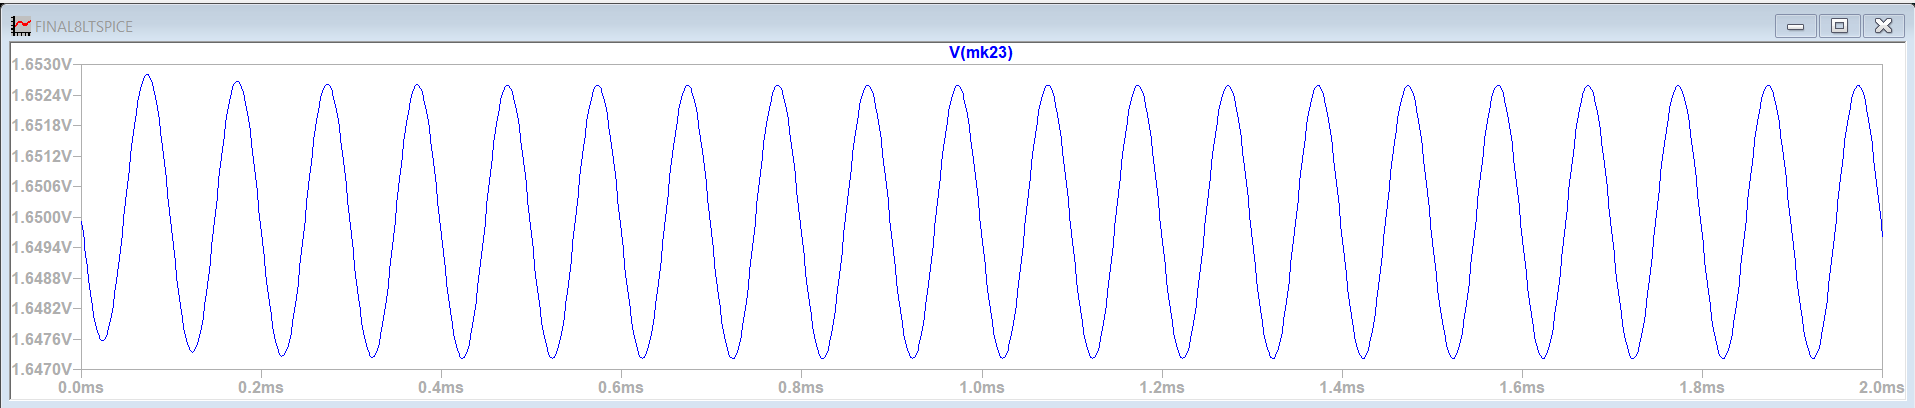
\includegraphics[width=1\linewidth]{imagess/current_700_70.png}
    \caption{Measured DUT current waveform obtained via shunt calculation.}
    \label{fig:eit_current}
\end{figure}
\subsubsection{Resistance calculation results}
The peak-to-peak current after shunt division is
\begin{equation}
I_\mathrm{pp} = \frac{V_\text{diff amplifier}}{R_\text{shunt}} = \frac{0.00539098~\mu\text{A}}{70~\Omega} \approx 77.014~\mu\text{A}.
\end{equation}
The peak-to-peak voltage measured across the DUT is
\[
V_\mathrm{pp} \approx 0.05351~\text{V}.
\]

\noindent Using the RMS relationship for a sinusoidal signal:
\[
V_\mathrm{rms} = \frac{V_\mathrm{pp}}{2\sqrt{2}}, \quad 
I_\mathrm{rms} = \frac{I_\mathrm{pp}}{2\sqrt{2}},
\]
the calculated resistance value confirms that the measurement chain correctly recovers the resistance value :
\begin{equation}
R_\text{calculated} = \frac{V_\mathrm{rms}}{I_\mathrm{rms}} 
= \frac{0.2680724 / (2\sqrt{2})}{382.905 \times 10^{-6} / (2\sqrt{2})} 
\approx 694.808~\Omega.
\end{equation}


The table bellow summarizes the time-domain validation results of the EIT acquisition system using single-frequency excitation. For each known resistor, the measured voltage and current were used to compute the effective resistance, The results show excellent agreement with the known resistance values, with minor deviations due to measurement precision and the finite resolution of the simulated acquisition circuit. For low-resistance loads, the measured current approaches the injected current limit, while for very high-resistance loads, the measured current is small, as expected. Overall, these results confirm that the simulation accurately reproduces the expected behavior of the resistive DUT, validating the correctness of the measurement chain.
\begin{table}[H]
\centering
\label{tab:single_freq_verification}
\begin{tabular}{|p{3cm}|p{3cm}|p{3cm}|p{3cm}|}
\hline
\textbf{Known resistance (\(\Omega\))} & \textbf{Measured Voltage (V)} & \textbf{Measured current (\(\mu\)A)} & \textbf{Calculated resistance (\(\Omega\))} \\ \hline
10  & 0.00433 & 431.7  & 10.029 \\ \hline
50  & 0.01692 & 341.0 & 49.619 \\ \hline
100  & 0.02686 & 270.0 & 99.481 \\ \hline
700  & 0.05351 & 77.014 & 694.808 \\ \hline
1000 & 0.05669 & 56.428 & 1004.643 \\ \hline
5000 & 0.06295 & 12.442 & 5059.475 \\ \hline
10000 & 0.06395 & 6.504 & 9832.410 \\ \hline
100000 & 0.06412 & 0.64657 & 99169.463 \\ \hline

\end{tabular}
\end{table}



\paragraph{(B) Frequency-domain Verification Using multi-frequency Excitation.}\\
The current injection was modeled using a behavioral current source configured to generate 
a multisine waveform composed of two frequency components. The injected current is given by  

\begin{equation}
I(t) = 100~\mu A \cdot \sin(2\pi \cdot 9765.625 \cdot t) 
     + 100~\mu A \cdot \sin(2\pi \cdot 49804.6875 \cdot t).
\end{equation}

This dual-tone excitation allows the system to be tested at two different frequency bands 
simultaneously, which is crucial for assessing multi-frequency EIT performance.
With multi-sine excitation, the complex impedance at each tone is estimated as
\begin{equation}
Z(f_k) \;=\; \frac{\mathcal{F}\{v(t)\}\big|_{f_k}}{\mathcal{F}\{i(t)\}\big|_{f_k}},
\quad
|Z(f_k)| = \frac{|V(f_k)|}{|I(f_k)|},\;
\angle Z(f_k) = \angle V(f_k) - \angle I(f_k),
\end{equation}
using the LTspice FFT on the voltage across and the current through the DUT. For a purely resistive load, \(|Z(f_k)| \approx R_\text{known}\) and \(\angle Z(f_k) \approx 0^\circ\) across tones (small deviations can occur from parasitics).\\
The time-domain waveforms for both the injected current and measured voltage are shown in the figures 3.15 and 3.16 . The multisine nature of the excitation is clearly visible in both signals, with the superposition of the two frequency components creating the characteristic beating pattern.
\begin{figure}[H]
    \centering
    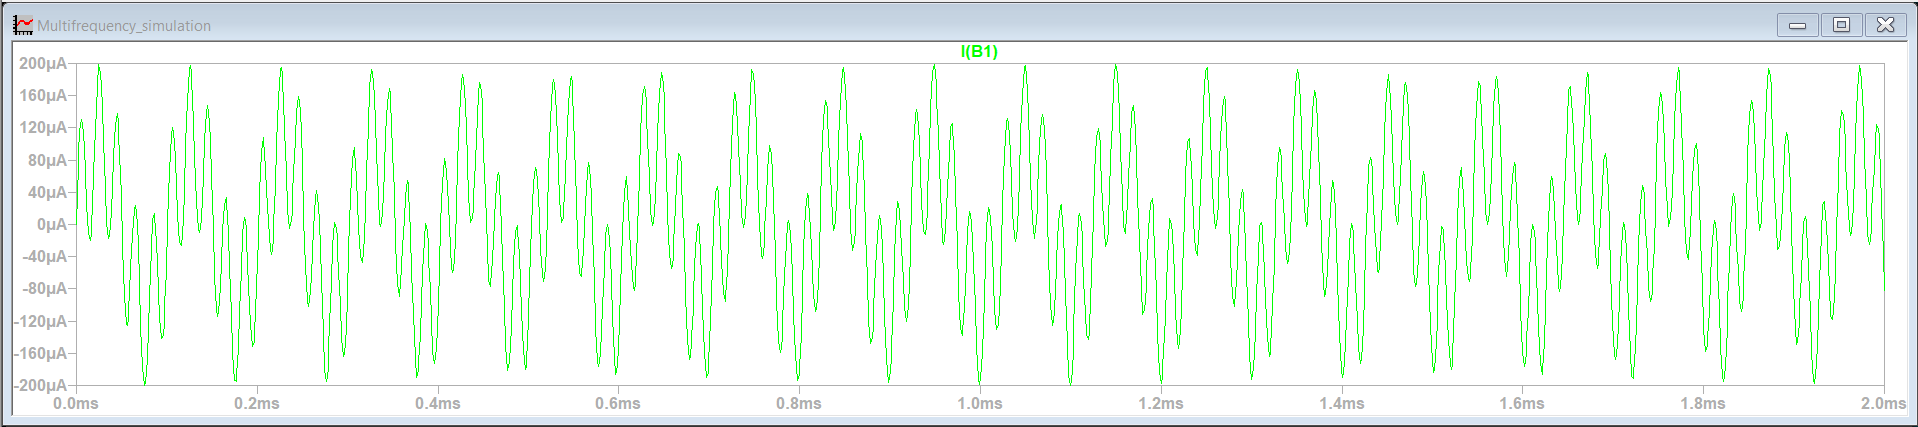
\includegraphics[width=1\textwidth]{imagess/injected_current_multifrequency.png}
    \caption{Injected current $I(t)$ .}
    \label{fig:current_time}
\end{figure}
\begin{figure}[H]
    \centering
    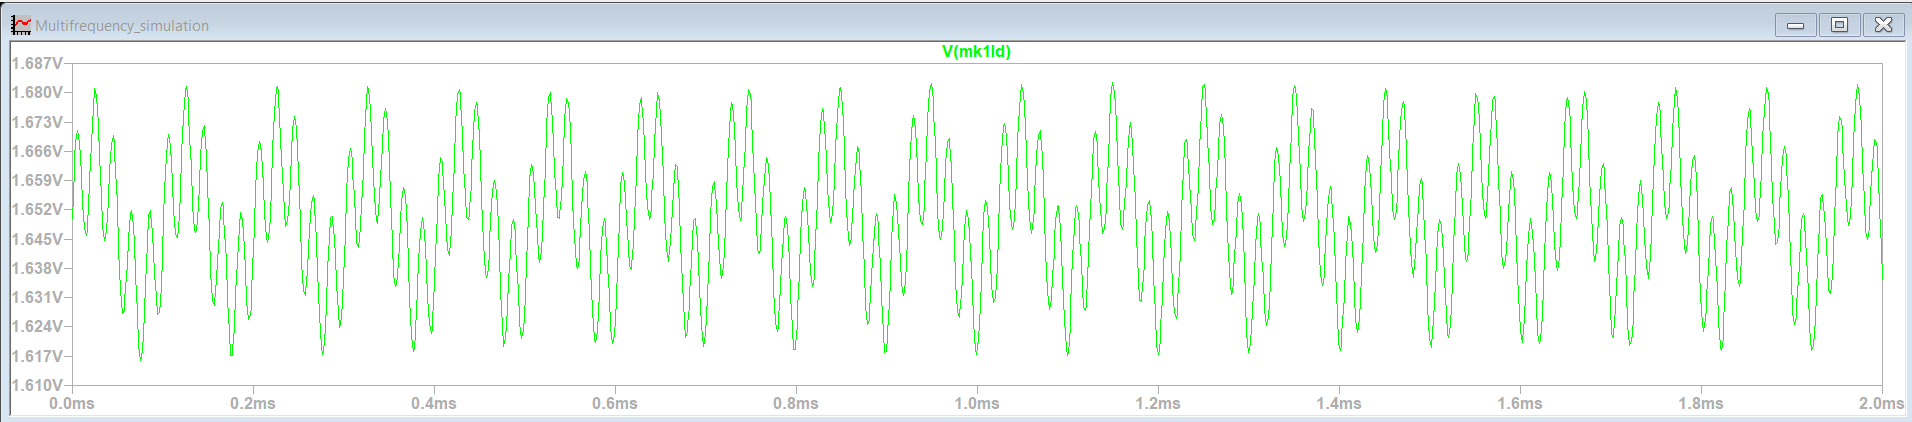
\includegraphics[width=1\textwidth]{imagess/voltage_multifrequency.png}
    \caption{Measured voltage $V(t)$.}
    \label{fig:voltage_time}
\end{figure}

The frequency-domain behavior of the simulated signals was analyzed using the Fast Fourier Transform (FFT). 
The spectra of the current and voltage waveforms exhibit distinct peaks at the two excitation frequencies, 
as shown in Figures~\ref{fig:fft_current} and~\ref{fig:fft_voltage}. 
The clean separation of frequency components confirms the effectiveness of the multisine excitation strategy 
for enabling simultaneous multi-frequency measurements.

\begin{figure}[H]
    \centering
    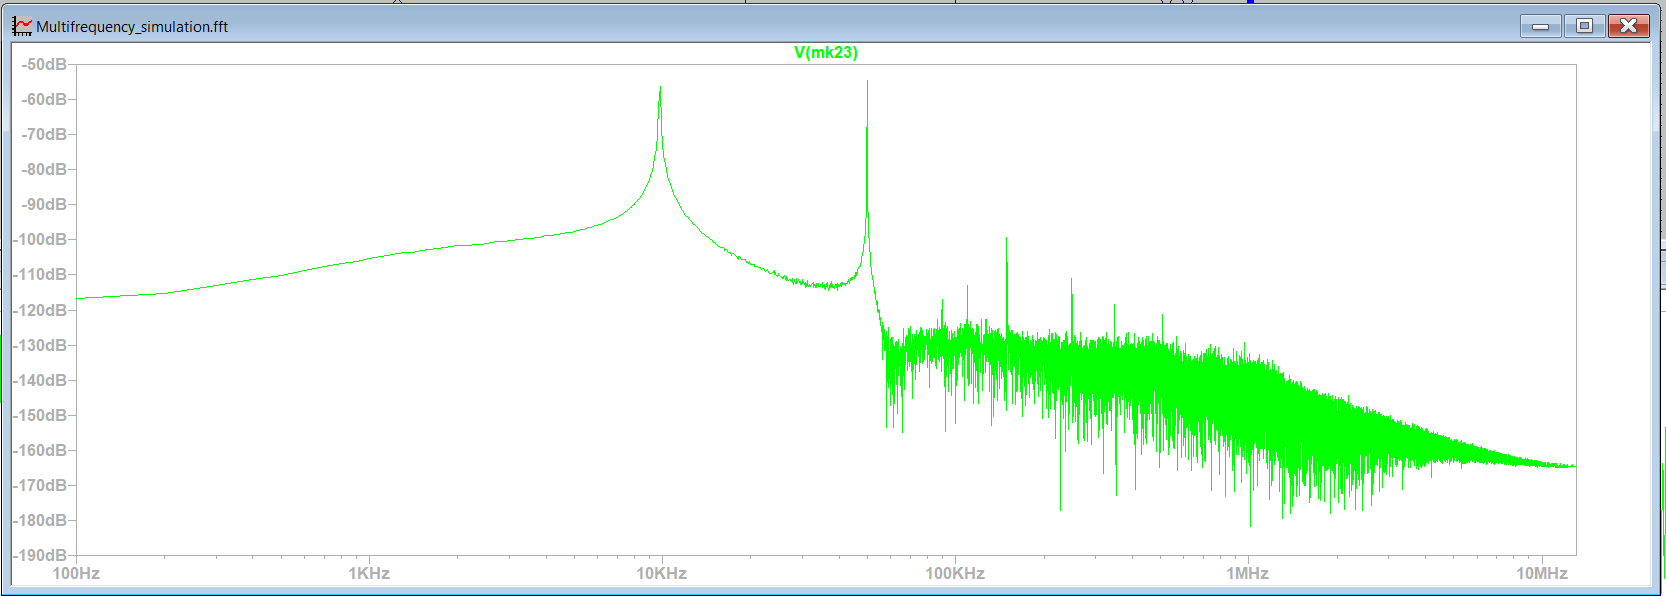
\includegraphics[width=0.9\textwidth]{imagess/FFT_ltspice_current.png}
    \caption{FFT spectrum of the simulated current signal.}
    \label{fig:fft_current}
\end{figure}

\begin{figure}[H]
    \centering
    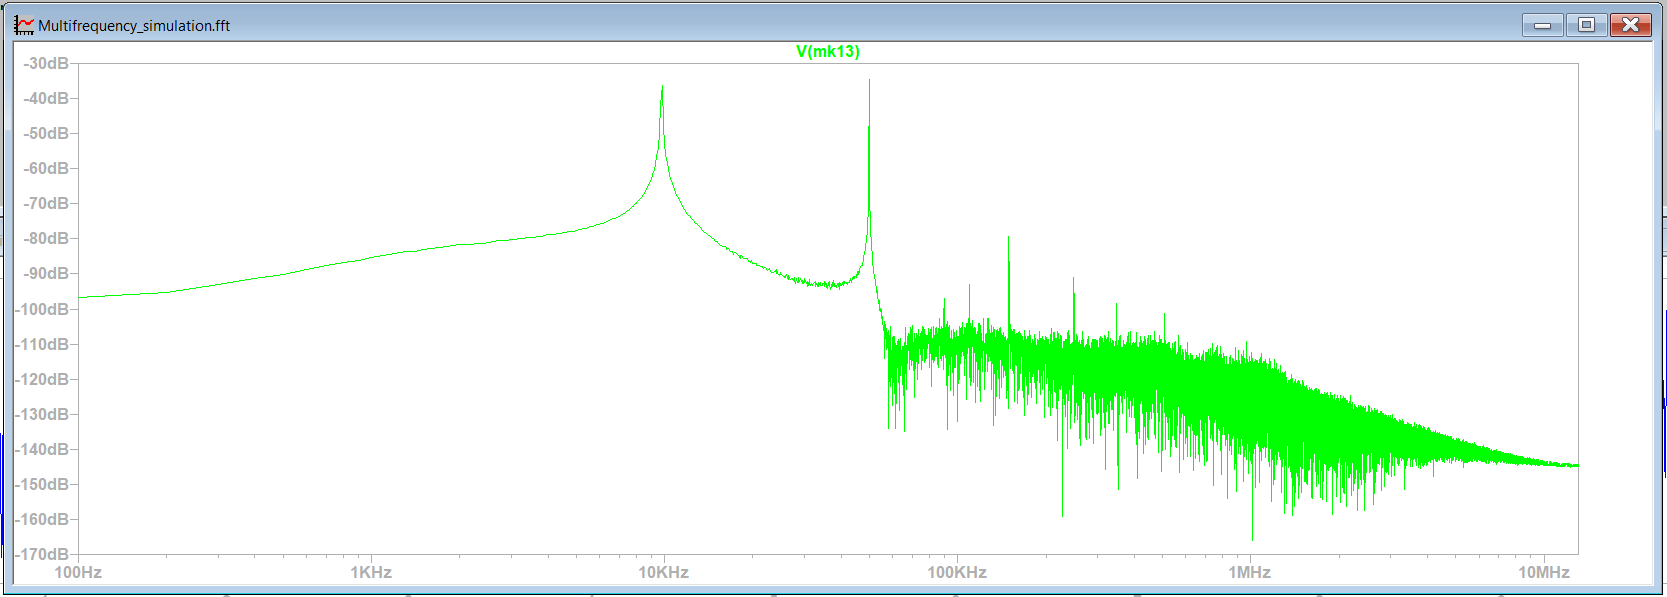
\includegraphics[width=0.9\textwidth]{imagess/FFt_ltspice_voltage.png}
    \caption{FFT spectrum of the simulated voltage signal.}
    \label{fig:fft_voltage}
\end{figure}


\subsubsection{Resistance calculation results}

To validate the impedance extraction methodology, a purely resistive reference load of 
$700~\Omega$ was implemented in LTspice. 
The current and voltage signals were processed via FFT, and the complex impedance was calculated. 
The resulting impedance values at the two excitation frequencies are summarized in Table~\ref{tab:impedance_results}.

\begin{table}[H]
    \centering
    \caption{Impedance extraction results from FFT analysis ($R_{\text{shunt}} = 70~\Omega$).}
    \label{tab:impedance_results}
    \begin{tabular}{|c|c|c|c|c|c|c|}
    \hline
    \textbf{Freq.} & \textbf{$|V(f)|$} & \textbf{$\angle V(f)$} & \textbf{$|I(f)|$} & \textbf{$\angle I(f)$} & \textbf{$|Z(f)|$} & \textbf{$\angle Z(f)$} \\
    \textbf{(kHz)} & \textbf{(mV)} & \textbf{(°)} & \textbf{($\mu$A)} & \textbf{(°)} & \textbf{($\Omega$)} & \textbf{(°)} \\
    \hline
    9.794  & 15.01 & -135.84 & 21.69 & 29.42 & 692.0 & -165.3 \\
    \hline
    49.802 & 18.14 & -92.00  & 24.51 & 81.19 & 740.1 & -173.2 \\
    \hline
    \end{tabular}
\end{table}

The extracted impedance magnitudes were $692.0~\Omega$ at 9.794~kHz and $740.1~\Omega$ at 49.802~kHz. 
These values are in close agreement with the theoretical $700~\Omega$ reference load, 
demonstrating the validity of the measurement chain. 
The small deviations in magnitude, together with the observed negative phase angles 
($-165.3^\circ$ and $-173.2^\circ$ instead of $0^\circ$), are attributed to numerical 
artifacts from the FFT process as well as parasitic elements inherent in the simulated setup.



The calculated values confirm that the expected $700~\Omega$ resistance is correctly 
recovered at both excitation frequencies. 
Importantly, since the two tones were applied simultaneously, this result validates not only the impedance 
extraction accuracy at individual frequencies but also the ability of the system to resolve 
multiple spectral components without crosstalk. 
This demonstrates that the FFT-based method can reliably extract impedance information in a 
simultaneous multi-frequency scenario, which is a key requirement for practical EIT systems. 
Consequently, this validation step establishes confidence in the measurement chain and provides 
a robust baseline before extending the approach to more complex DUTs and tissue-equivalent circuits.


\subsection{Circuit design}

After verifying the design through simulations, the circuit was implemented in EasyEDA to create an accurate schematic. The layout and connections were carefully checked to reduce unwanted parasitic effects that could affect high-frequency signal accuracy.

\begin{figure}[H]
    \centering
    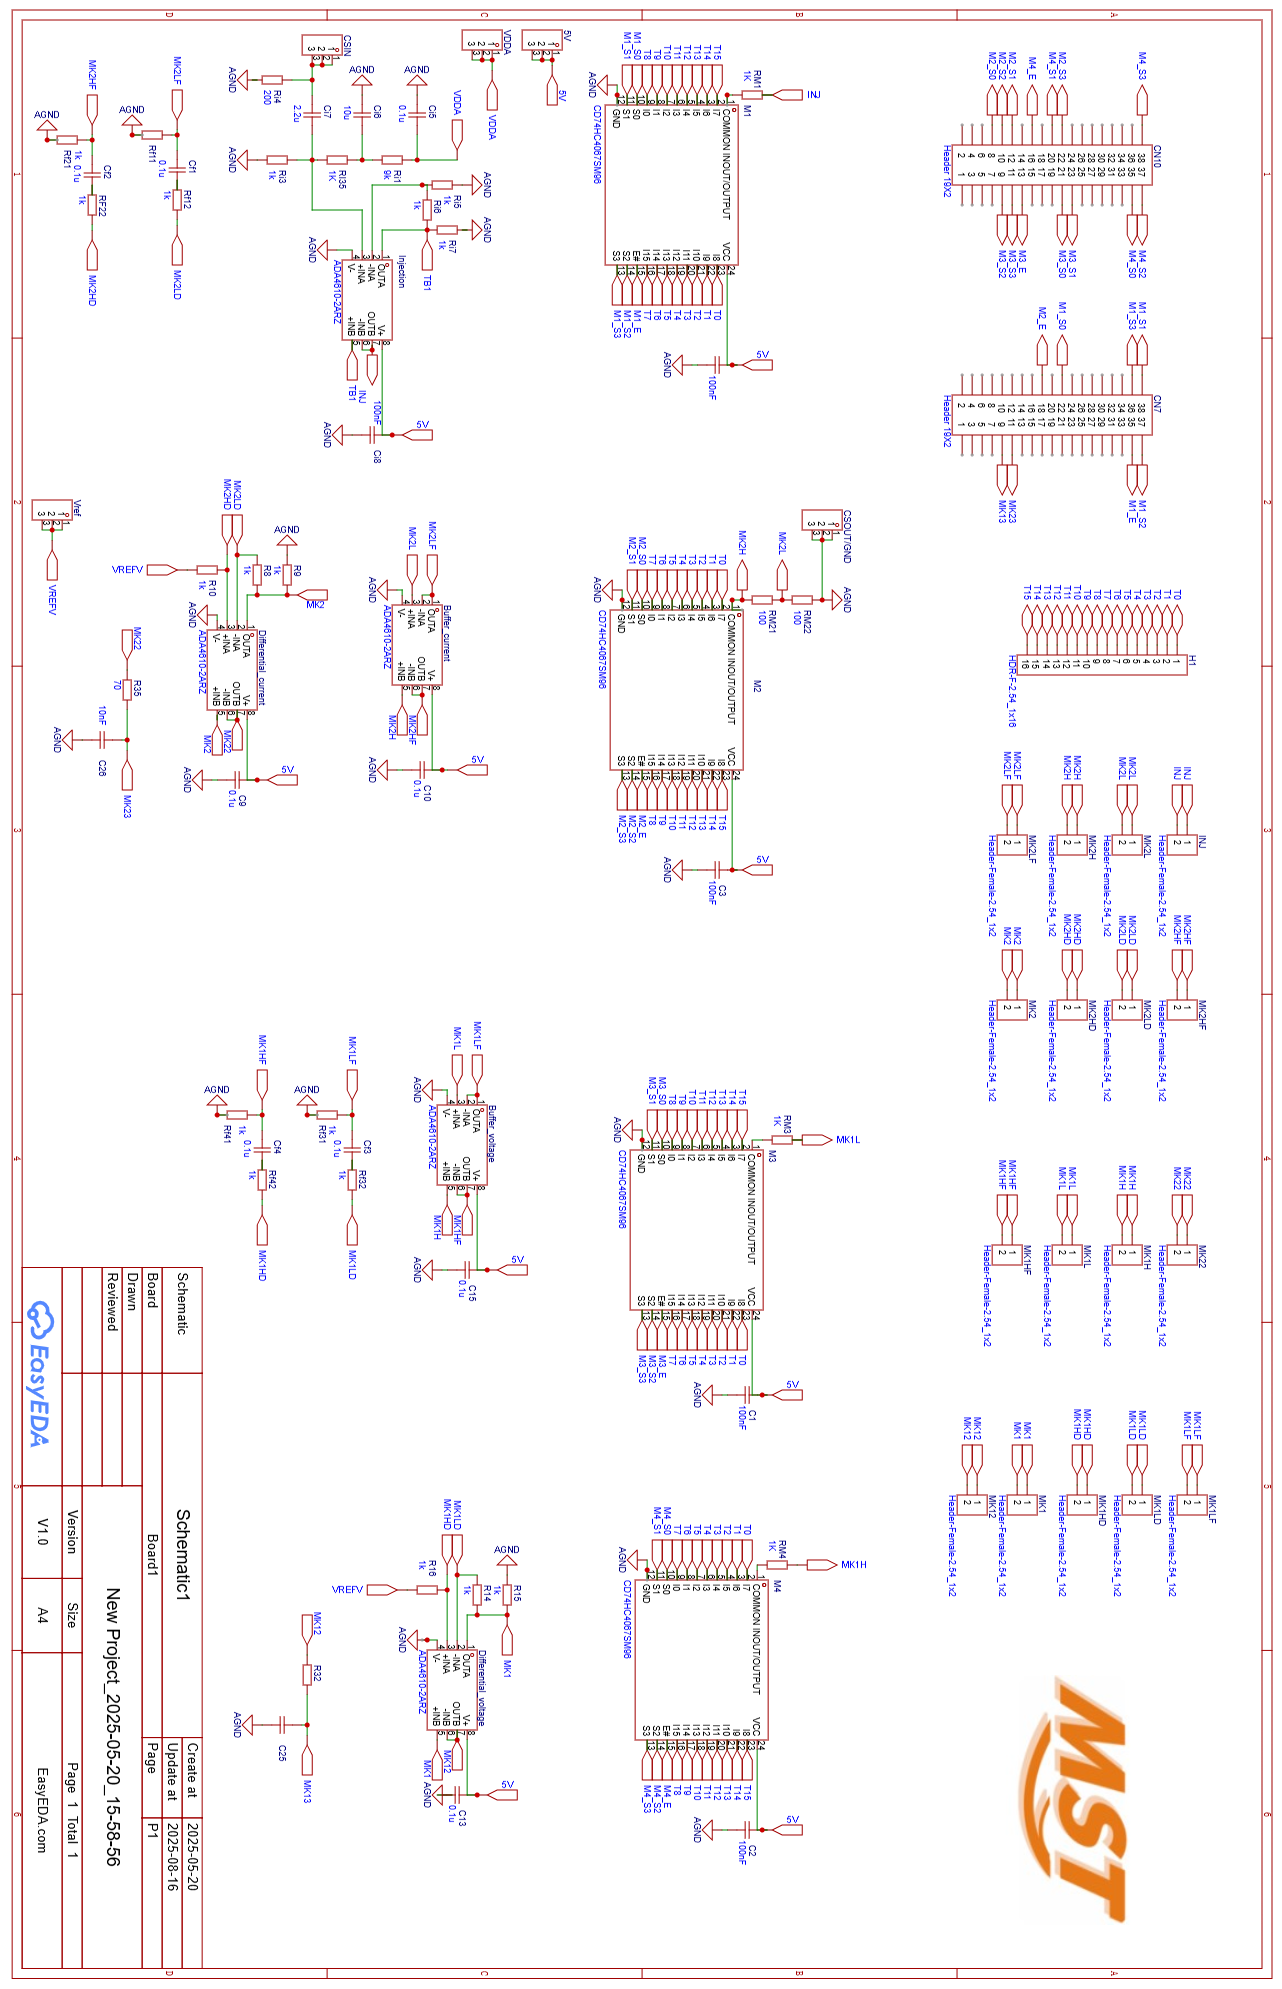
\includegraphics[width=0.8\textwidth]{imagess/SCH_Schematic1_1-P1_2025-08-16 (1).png}
    \caption{EasyEDA schematic of the EIT acquisition circuit.}
    \label{fig:easyeda_schematic}
\end{figure}

\subsection{PCB layout and routing}
  
The PCB layout was designed to minimize signal integrity, power supply stability, and noise, while not driving the overall size of the design up or making it unproducible. To achieve this, a two-layer PCB design was used, where one layer was completely utilized as a continuous ground plane and the second was utilized for the 5 V power plane and signal routing.

\begin{itemize}
    \item \textbf{Layer allocation:}  
    \begin{itemize}
        \item \textbf{Top layer:} Utilized solely as a continuous ground plane, providing a low-
impedance return path to every signal and suppression of electromagnetic inter-
ference (EMI). This also simplified grounding sensitive analog circuits and
shielding against switching noise.  
        \item \textbf{Bottom Layer:}Labeled as the 5 V distribution plane, it supported the main
supply rail with extra signal traces. The power was routed evenly around the
board, with high-current paths using wider traces.  
    \end{itemize}


    \item \textbf{Signal routing:}  
    Sensitive analog signals were routed with minimal trace length to
reduce susceptibility to pickup by noise. Traces were taken wherever possible directly
over the solid ground plane for controlled impedance and reduced loop areas.
High-frequency excitation signals were careful routed to avoid crosstalk, and digital lines
were not routed parallel to each other.

    \item \textbf{Power integrity and decoupling:}  
    Power Integrity and Decoupling: Since the 5 V supply was delivered by the bottom plane, local decoupling capacitors were placed near each component (e.g.,
the microcontroller, op-amps, and voltage regulator) in stabilizing the voltage at the current point of load and in removing transient oscillations. Bulk capacitors were distributed across near the power input connector to ensure stable operation under sustained dynamic load conditions.  

    \item \textbf{Grounding strategy:}  
    A complete dedicated ground plane layer was used to provide short and direct path for all components to reference potential and keep ground noise to a minimum. This reduced ground loops and optimized overall signal quality. 

    \item \textbf{Design rule checks (DRC):}  
    Layout was verified to meet the PCB manufacturer's trace width, clearance, via size, and annular ring requirements, ensuring fabrication-free trouble.
    \item \textbf{Tool and Visualization:}  
  Tool and Visualization: The PCB was designed and verified using EasyEDA, providing both electric rule checking and advanced visualization capabilities. \\

\end{itemize}
Figure~\ref{fig:pcb_all} presents the complete design of the PCB in EasyEDA, including both the top and bottom layer routings as well as the corresponding 3D views.
\begin{figure}[H]
    \centering
    % (a) Top layer PCB
    \begin{subfigure}[b]{0.45\textwidth}
        \centering
        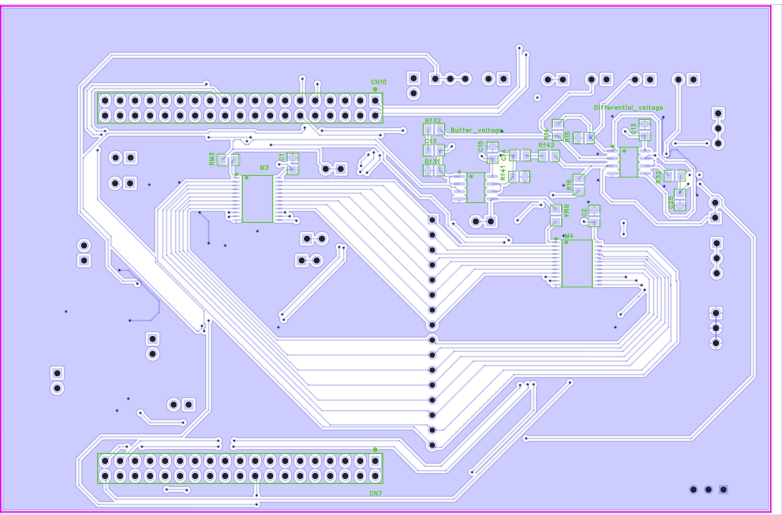
\includegraphics[width=\textwidth]{imagess/top_layer.jpg}
        \caption{PCB layout and routing (top layer view).}
        \label{fig:pcb_layout3}
    \end{subfigure}
    \hfill
    % (b) Bottom layer PCB
    \begin{subfigure}[b]{0.45\textwidth}
        \centering
        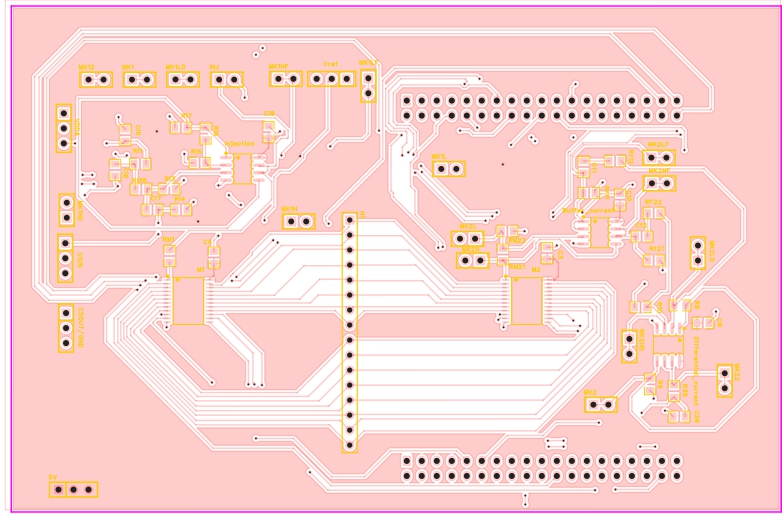
\includegraphics[width=\textwidth]{imagess/PCB_PCB1_2025-08-17 (1)_page-0001.jpg}
        \caption{PCB layout and routing (bottom layer view).}
        \label{fig:pcb_layout4}
    \end{subfigure}
    
    \vspace{0.5cm} % spacing between rows
    
    % (c) 3D Top view
    \begin{subfigure}[b]{0.45\textwidth}
        \centering
        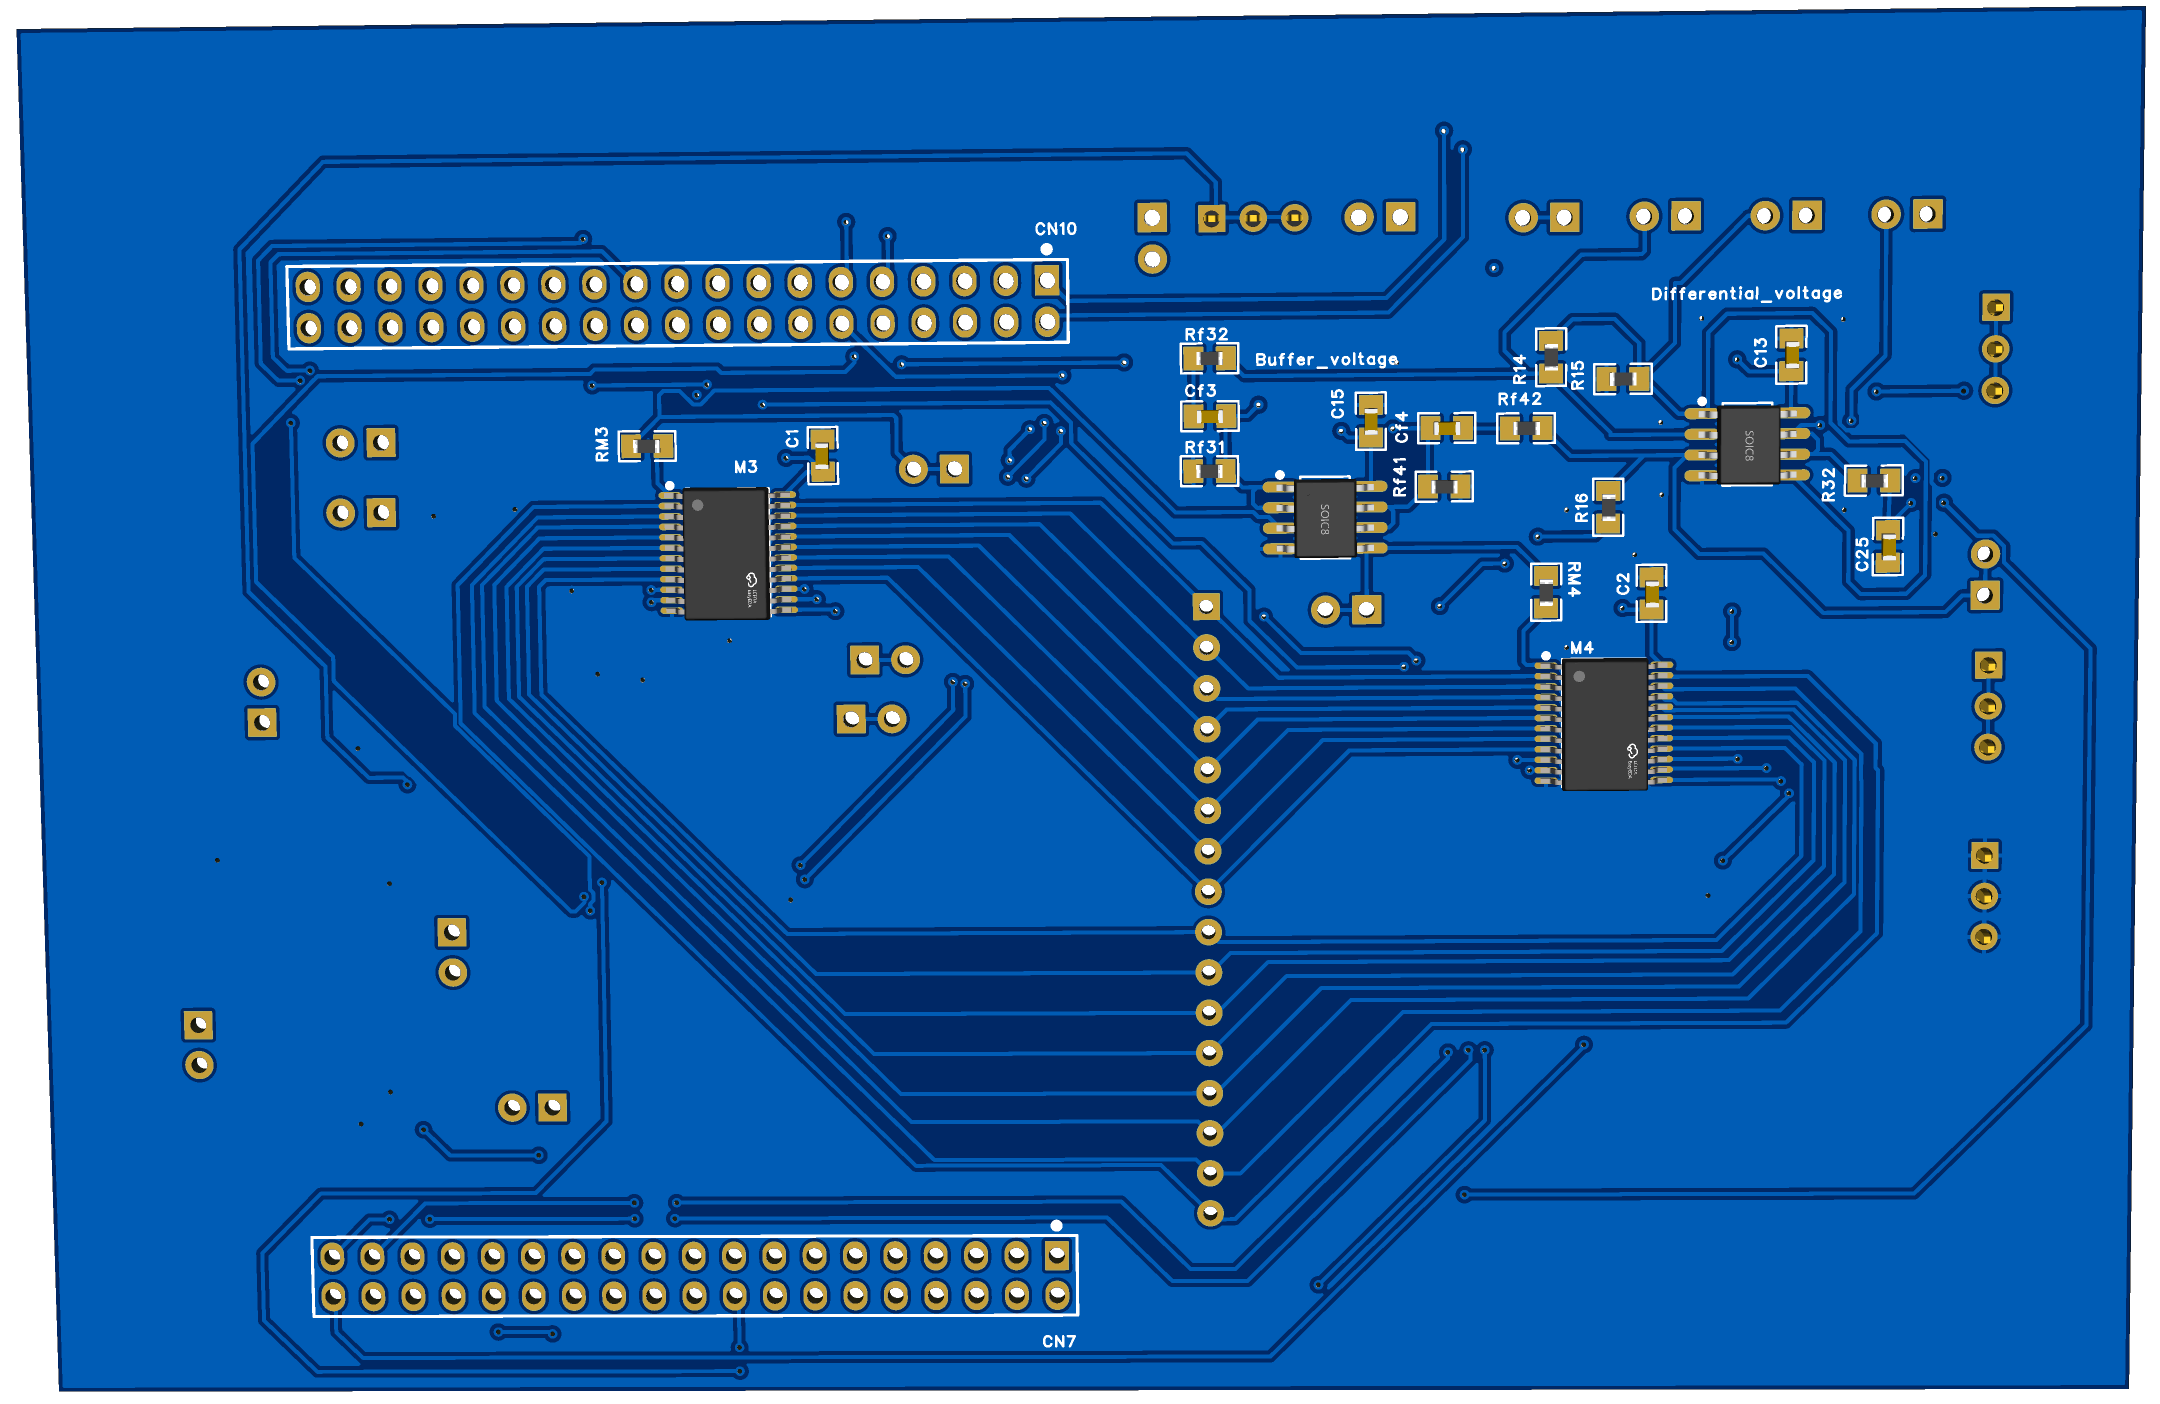
\includegraphics[width=\textwidth]{imagess/3D_PCB1_2025-07-16 (1).png}
        \caption{3D layout (top view).}
        \label{fig:pcb_layout}
    \end{subfigure}
    \hfill
    % (d) 3D Bottom view
    \begin{subfigure}[b]{0.45\textwidth}
        \centering
        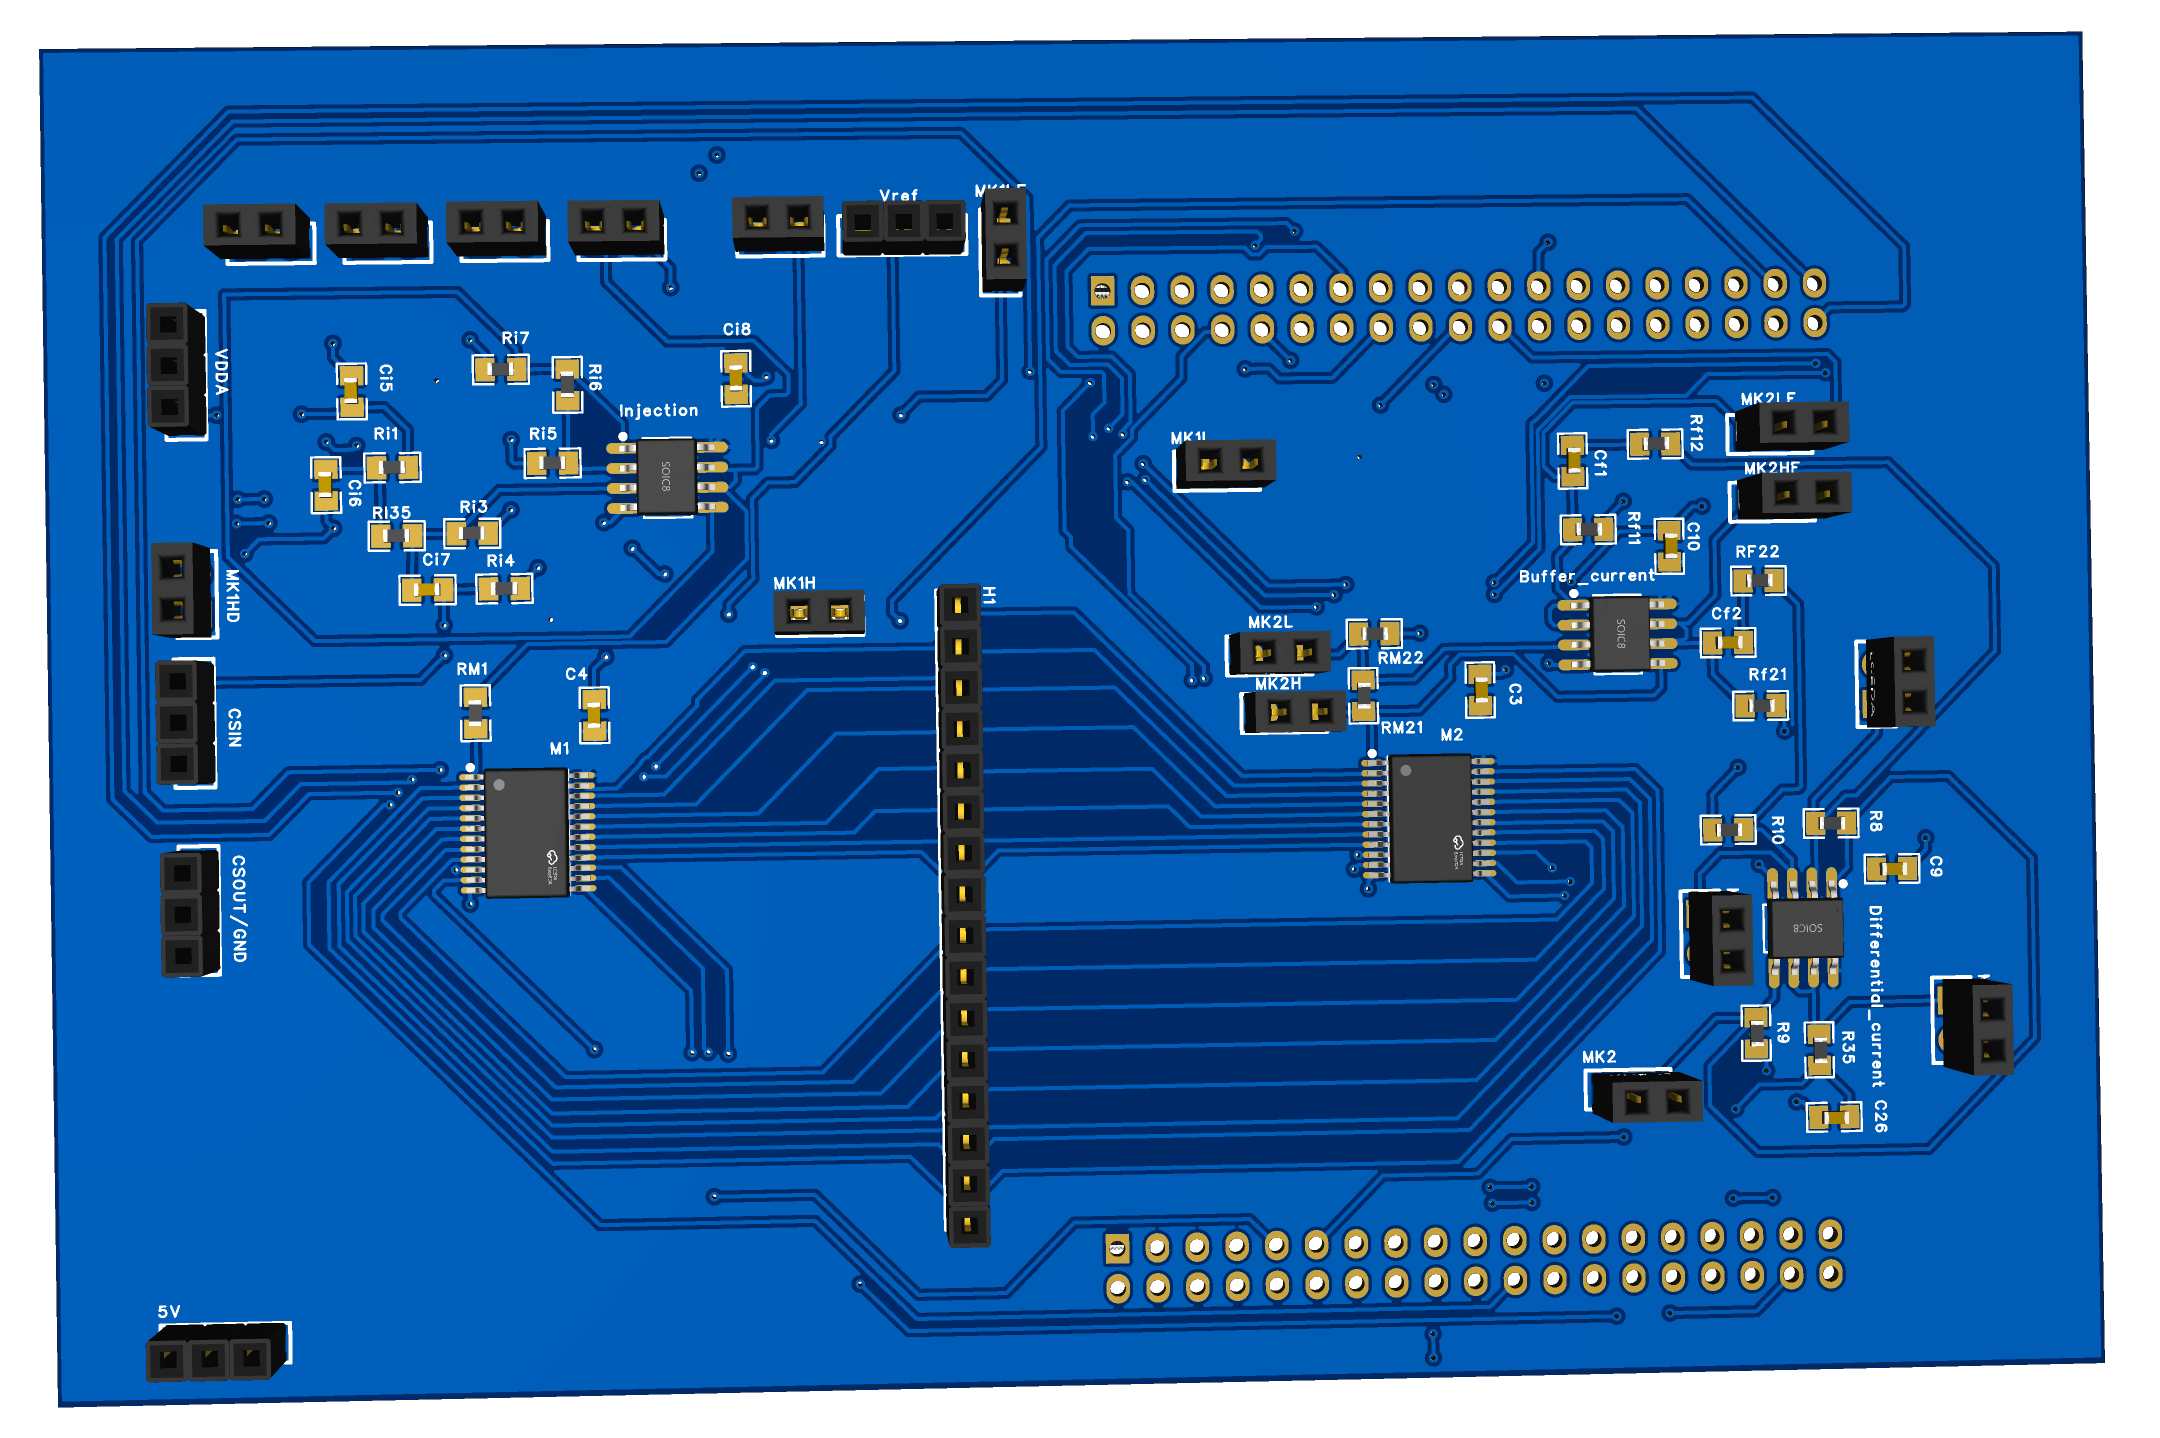
\includegraphics[width=\textwidth]{imagess/3D_PCB1_2025-08-16 (2).png}
        \caption{3D layout (bottom view).}
        \label{fig:pcb_layout2}
    \end{subfigure}
    
    \caption{PCB layouts and 3D views in EasyEDA: (a) top layer routing, (b) bottom layer routing, (c) 3D top view, (d) 3D bottom view.}
    \label{fig:pcb_all}
\end{figure}
\subsection{Generation of manufacturing documentation } 
  Figure~\ref{fig:drc} shows the rule configuration inside EasyEDA.

\begin{figure}[H]
\centering
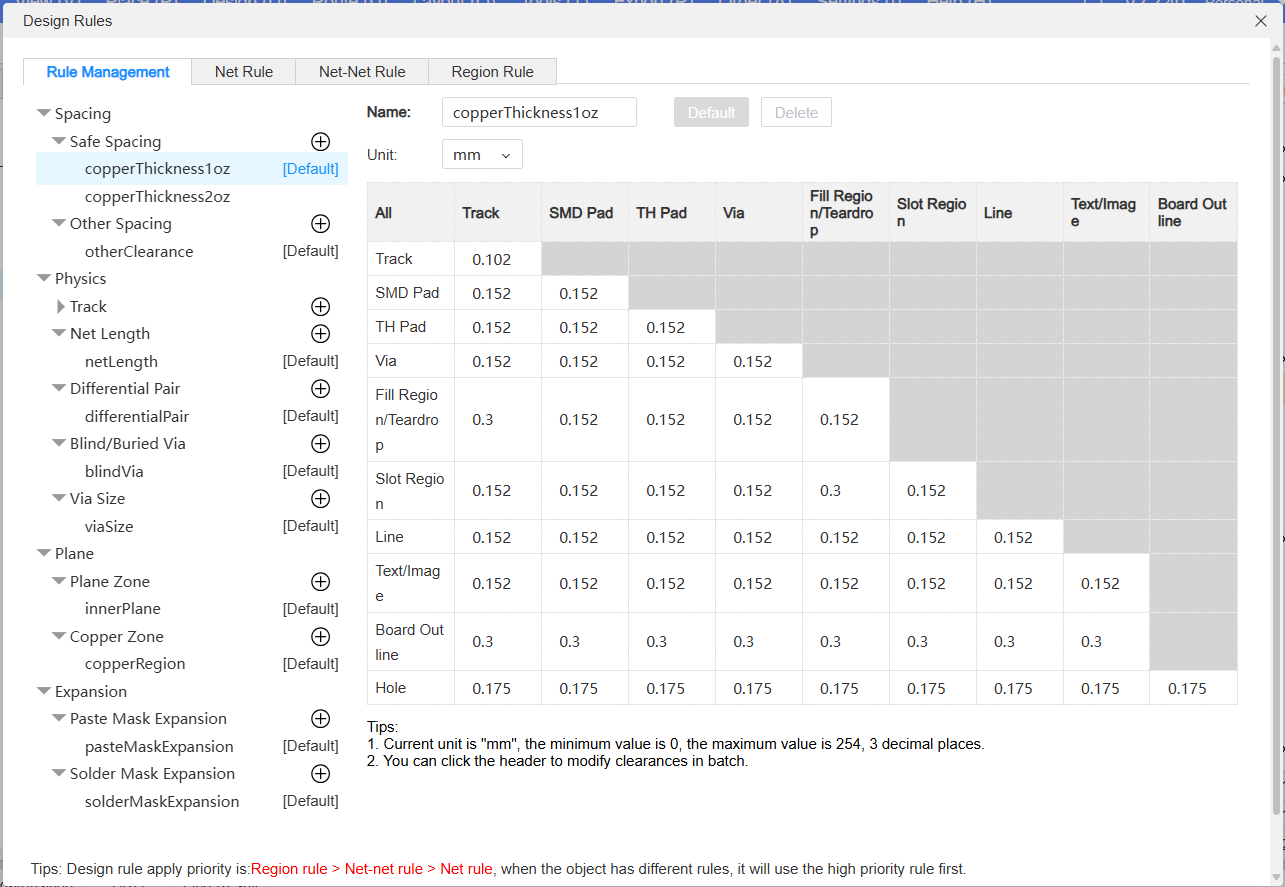
\includegraphics[width=0.6\textwidth]{imagess/Screenshot 2025-08-17 104409.png}
\caption{Design rule settings in EasyEDA aligned with Fischer’s manufacturing constraints.}
\label{fig:drc}
\end{figure}

After validating the design with the DRC tool, the Gerber and BOM files were generated and subsequently uploaded to Fischer’s online platform. This ensured that the board specifications sizes were fully compatible with the manufacturer’s production capabilities, guaranteeing reliable and reproducible fabrication.

\begin{table}[H]
\centering
\caption{Fischer PCB Manufacturing Rules for 2-Layer Boards\cite{FischerPCB}}
\begin{tabular}{|c|c|c|}
\hline
\textbf{Copper Thickness} & \textbf{Min. Trace Width} & \textbf{Min. Spacing} \\
\hline
35\,µm (1 oz)  & 150\,µm (6 mil)  & 150\,µm (6 mil) \\
\hline
70\,µm (2 oz)  & 200\,µm (8 mil)  & 200\,µm (8 mil) \\
\hline
105\,µm (3 oz) & 300\,µm (12 mil) & 350\,µm (14 mil) \\
\hline
\multicolumn{3}{|c|}{\textbf{Minimum finished drill diameter: 0.3\,mm}} \\
\hline
\end{tabular}
\end{table}
\section{STM32-based excitation and acquisition}

This section presents the embedded system implementation on the STM32 microcontroller, 
covering the generation of excitation signals, multiplexer control, and synchronized 
data acquisition. Screenshots from STM32CubeMX, oscilloscope captures, and configuration 
parameters are provided to illustrate the design.  

\subsection{Excitation signal generation}

The excitation signal was generated using the \textbf{DAC peripheral}, driven by a timer 
(\texttt{TIMx}) to ensure deterministic sampling. The DAC waveform was based on a 
precomputed sine lookup table stored in memory.  

To satisfy the Nyquist criterion and ensure accurate waveform synthesis, the sampling 
frequency was chosen to be at least 2 times higher than the maximum excitation frequency 
of 500~kHz, resulting in a DAC sampling rate of $\geq 1$~MHz.  

The timer frequency was computed as\cite {ST_RM0090}:  

\begin{equation}
f_{\text{timer}} = \frac{f_{\text{clk}}}{(PSC+1)(ARR+1)}
\end{equation}


where $f_{\text{clk}}$ is the system clock frequency, $PSC$ is the prescaler value, and $ARR$ 
is the auto-reload register value.  

\subsubsection*{Parameters}
\begin{itemize}
    \item Prescaler (PSC): \texttt{1}
    \item Auto-reload register (ARR): \texttt{39}
    \item Resulting timer frequency: \texttt{1M} Hz
    \item DAC resolution: 12-bit
\end{itemize}

\end{figure}
To acquire both the voltage and current signals simultaneously, two ADC channels were configured: \texttt{ADC1} for voltage measurement and \texttt{ADC2} for current measurement. In order to guarantee synchronization between the two channels, both were triggered by the same timer (\texttt{Timer~2}). This ensures that the sampling of voltage and current occurs at exactly the same instants, which is crucial for accurate impedance reconstruction.

To further optimize the acquisition process, Direct Memory Access (DMA) was enabled. The use of DMA allows the sampled data from both ADCs to be transferred directly into memory without CPU intervention, thereby improving system efficiency and reducing latency.





The ADC channels were sampled using the STM32 HAL library. To start the acquisition, the ADCs were first calibrated, then started in DMA mode, and finally triggered by Timer~2. This process was implemented through the following functions:


\begin{itemize}
    \item \texttt{HAL\_ADCEx\_Calibration\_Start} performs a single-ended calibration of ADC1.
    \item \texttt{HAL\_ADC\_Start\_DMA} starts the ADC in DMA mode, storing 1024 samples into \\\texttt{adcValueArray}.
    \item \texttt{HAL\_TIM\_Base\_Start} starts Timer~2, which triggers the ADC at the configured sampling frequency of 5~MHz.
\end{itemize}

\subsection{Injection control}
The electrode switching module is a crucial part of the EIT system. The number of electrodes directly impacts several key aspects of the EIT system, such as measurement speed, computational load for image reconstruction, and image resolution. Commonly used configurations in EIT systems include 8, 16, 32, or 64 electrodes. Systems with fewer electrodes offer simpler and more reliable hardware designs but result in lower imaging resolution and reduced detail in reconstructed images. Conversely, systems with a larger number of electrodes, such as 64, can acquire more measurement data, improving imaging quality. However, this also leads to longer acquisition times, which may restrict the system’s practical applications.

Considering these trade-offs, a 16-electrode configuration was selected for this work. This choice provides a balanced compromise between hardware complexity, system reliability, and imaging performance.

In any EIT system, both the current injection electrodes and the voltage measurement electrodes need to be switched rapidly and accurately. Multiplexers are used to perform this switching. 

Each multiplexer has five control inputs: the enable pin (\texttt{E}) and four selection bits (\texttt{S0-S3}), which allow access to all 16 channels. For this design, four multiplexers are used in total: two for the current injection electrodes and two for the voltage measurement electrodes. Controlling these four multiplexers requires 20 GPIO pins. The STM32G4 microcontroller used in this project has 144 available pins, allowing sufficient resources to manage all multiplexers along with other required functions.
Four analog multiplexers were programmed through GPIO pins. A control algorithm cycles 
through electrode pairs in an adjacent injection pattern. 


The logic is implemented using nested loops, as illustrated in Figure~\ref{fig:adjacent_injection}.
\begin{figure}[H]
    \centering
    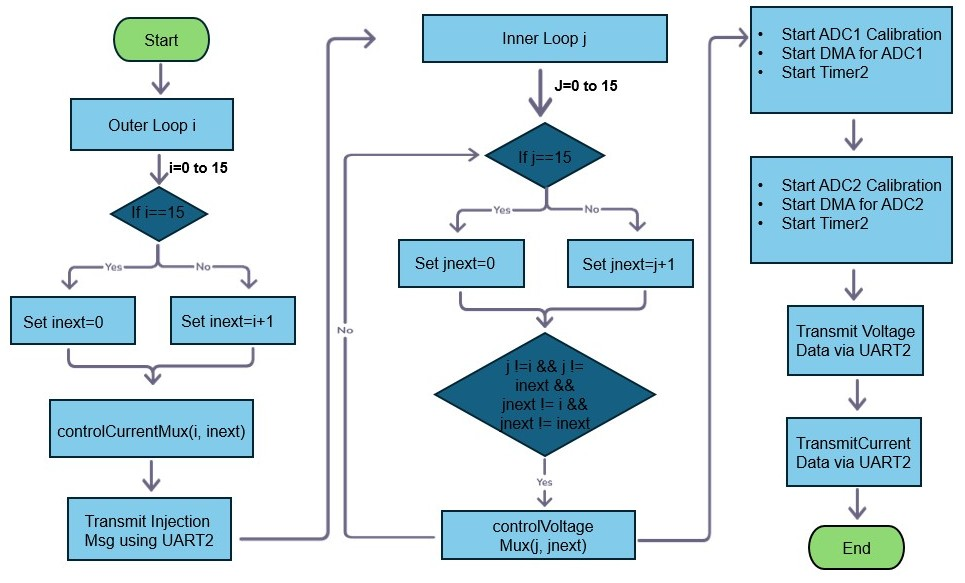
\includegraphics[width=1\textwidth]{imagess/injection_diagram.jpg}
    \caption{Diagram of adjacent electrode injection scheme using 4 multiplexers.}
    \label{fig:adjacent_injection}
\end{figure}

\begin{itemize}
    \item \textbf{Outer loop (\texttt{i})}: selects the current injection pair.
    \item \textbf{Inner loop (\texttt{j})}: controls the voltage measurement channels.
    \item The \texttt{inext} index ensures adjacent injection, wrapping around the electrodes:
    \[
    \texttt{inext} = 
    \begin{cases}
    0 & \text{if } i = 15 \\
    i+1 & \text{otherwise}
    \end{cases}
    \]
\end{itemize}

Two control functions were implemented in the firmware to manage this switching:

\begin{itemize}
    \item \texttt{controlCurrentMux(int channelIn, int channelOut)}  
    This function configures the multiplexers that connect the current source to the selected electrode pair. The parameters \texttt{channelIn} and \texttt{channelOut} correspond to the indices of the input and output electrodes, respectively. Each multiplexer address line (S0--S3) is driven by the STM32 GPIO pins using the \texttt{HAL\_GPIO\_WritePin()} function, which sets the binary control word according to the desired channel index:
    \[
    \text{MUX Address} = \bigl[b_3\; b_2\; b_1\; b_0 \bigr] \quad \Rightarrow \quad \text{Selected Electrode Channel}.
    \]

    \item \texttt{controlVoltageMux(int channelIn, int channelOut)}  
    This function operates in the same way, but for the voltage measurement electrodes. The input electrode (\texttt{channelIn}) and output electrode (\texttt{channelOut}) are selected through two multiplexers, with their address bits written via the microcontroller GPIO pins. This allows the system to measure the differential boundary voltage across the chosen electrode pair.
\end{itemize}

By abstracting the multiplexer control into these two functions, the electrode selection process becomes modular and easily programmable. During a full EIT measurement cycle, the firmware iterates through predefined electrode configurations, sequentially activating the appropriate pairs for current injection and voltage measurement. This automated switching is essential for reconstructing tomographic images, as it enables systematic data collection across all electrode combinations without manual reconfiguration.





\section{ Conclusion}
In this chapter, the process of designing the PCB was described in detail from layout, routing, design rule check, generation of Gerber and BOM files for safe man-
ufacturing. The STM32-based excitation and acquisition unit was installed,
encompassing DAC signal generation, multiplexer-driven electrode switching, and
synchronized ADC data acquisition. The 16-electrode configuration adopted
strikes a hardware complexity and imaging performance compromise, allowing for
systematic and automated data collection for EIT measurements.

\chapter*{chapter 4}
\markboth{Chapter 4 }{ Experimental results and validation
 } %pour afficher l'entete
 \addcontentsline{toc}{chapter}{IV  Experimental results and validation
 }

\textbf{\Huge Experimental results and validation
} 

\setcounter{chapter}{4}
\setcounter{section}{0}


\section{Introduction}
This chapter is dedicated to the validation of the developed EIT acquisition system in the frequency domain and via experimental imaging tests. Validation is initiated with managed measurements on a known resistance, which allows for quantitative assessment of the accuracy and consistency of the system's impedance estimate over different trials and frequencies. The results indicate how the selection of frequency affects reproducibility and sensitivity.

After this step, the system is tested under more realistic conditions with a water tank. Simultaneous multi-frequency excitations are introduced and reconstructed conductivity maps are computed to explore how the placement of objects affects the image result. This twofold strategy—numerical impedance verification and test-tank based reconstruction—assures that the system is tested both in measurement reliability as well as imaging performance, providing a basis for its use in tomographic investigations.
\section{Excitation signal generation}


This algorithm of signal generation was executed in Python to generate excitation signals automatically for various configurations, taking advantage of its scientific computing libraries for fast signal processing and visualization. The major libraries employed are:
\begin{itemize}
    \item NumPy: For numerics, array operations, and generating discrete fre-quency components. NumPy functions were employed to generate the multisine signals, carry out frequency quantization, and calculate the time-domain waveforms\cite{harris2020array}.

\item SciPy: The fft module was particularly used to calculate the Fast Fourier Transform
(FFT) of the synthesized signals, making possible the validation of frequency compo-
nents and their magnitudes\cite{virtanen2020scipy}.

\item Matplotlib:For plotting and visualization of time-domain waveforms and frequency-
domain spectra, with accurate placement of frequencies and phase distribution\cite{hunter2007matplotlib}.

\item Pandas:For structuring frequency component information and exportation of fre-
quency tables (original, quantized, and bin indices) for documentation and reference\cite{reback2020pandas}.
\end{itemize}
The generated signals were analyzed to assure
correct frequency positioning, phase allocation, and amplitude scaling.
\paragraph{2-Frequency multisine signal}  
The frequencies for the 2-frequency signal were chosen between 10 kHz and 50 kHz. The table below lists their original frequencies, quantized frequencies (based on FFT bin resolution), and their corresponding frequency bin indices.

\begin{table}[H]
    \centering
    \caption{Frequency components for the 2-frequency multisine}
    \label{tab:freq_2f}
    \begin{tabular}{|p{2cm}|p{4cm}|p{4cm}|p{3cm}|}
        \hline
        \textbf{Frequency No.} & \textbf{Original Frequency (Hz)} & \textbf{Quantized Frequency (Hz)} & \textbf{Frequency Bin Index} \\
        \hline
        1 & 10000.0000   & 9765.6250    & 10 \\
        \hline
        2 & 49999.9999  & 49804.6875  & 51 \\
        \hline
    \end{tabular}
\end{table}

Figure~\ref{fig:fft_2freq} shows the FFT magnitude spectra for the 2 frequencies configuration. The two distinct peaks confirm that both frequencies are correctly generated and isolated without spurious harmonics.

\begin{figure}[H]
    \centering
    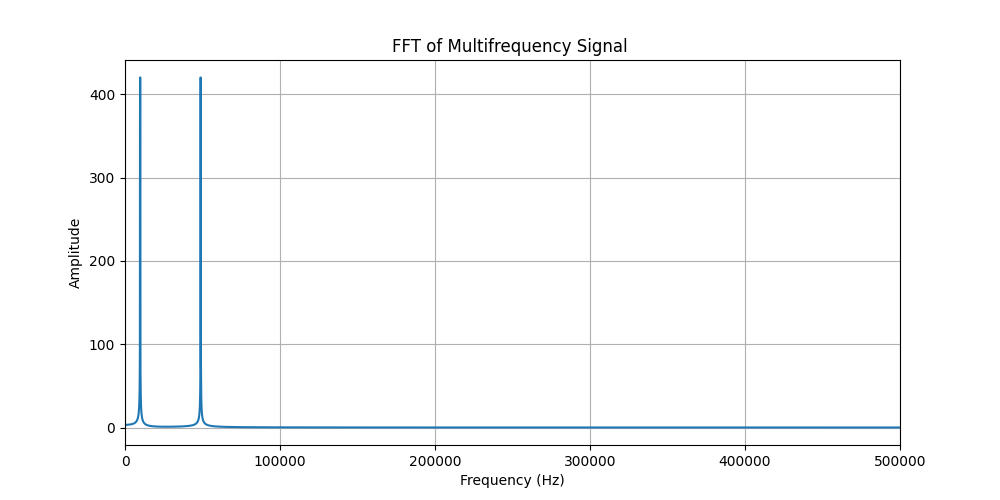
\includegraphics[width=0.9\linewidth]{imagess/FFT_2f.png}
    \caption{FFT magnitude spectrum of the 2-frequency multisine.}
    \label{fig:fft_2freq}
\end{figure}

\paragraph{5-Frequency multisine signal}  
The 5-frequency multisine signal was designed with frequencies spanning from 10 kHz to 250 kHz. Table~\ref{tab:freq_5f_corrected} lists the original frequencies, their quantized equivalents based on FFT resolution, and the corresponding frequency bin indices.

\begin{table}[H]
    \centering
    \caption{Frequency components for the 5-frequency multisine}
    \label{tab:freq_5f_corrected}
    \begin{tabular}{|p{2cm}|p{4cm}|p{4cm}|p{3cm}|}
        \hline
        \textbf{Frequency No.} & \textbf{Original frequency (Hz)} & \textbf{Quantized frequency (Hz)} & \textbf{Frequency bin index} \\
        \hline
        1 & 10000.0000       & 9765.6250     & 10  \\
        \hline
        2 & 22360.6798       & 22460.9375    & 23  \\
        \hline
        3 & 50000.0000       & 49804.6875    & 51  \\
        \hline
        4 & 111803.3989      & 111328.1250   & 114 \\
        \hline
        5 & 249999.9999      & 250000.0000   & 234 \\
        \hline
    \end{tabular}
\end{table}
 Figure~\ref{fig:fft_6freq} shows  the FFT magnitude spectra for the 5 frequencies configuration. The five spectral peaks appear at the expected logarithmically spaced positions, demonstrating the algorithm’s ability to handle higher-order configurations while preserving spectral purity and avoiding intermodulation artifacts.
\begin{figure}[H]
    \centering
    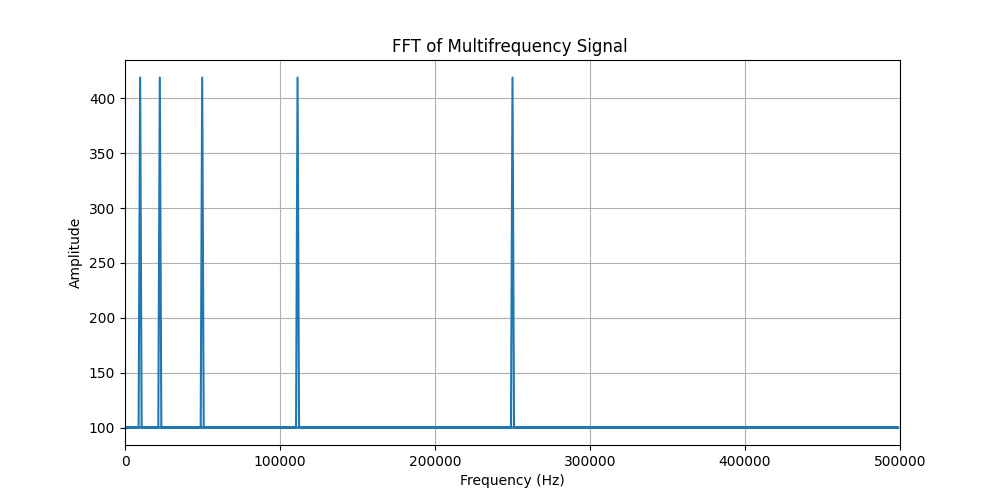
\includegraphics[width=0.9\linewidth]{imagess/FFT_5f.png}
    \caption{FFT magnitude spectrum of the 5-frequency multisine.}
    \label{fig:fft_6freq}
\end{figure}



\section{Experimental setup}
The experimental setup for validating the EIT system is shown in Figure~\ref{fig:setup}. The hardware consists of a Voltage-Controlled Current Source (VCCS) and the custom-designed EIT PCB connected to a circular tank equipped with 16 electrodes. The electrodes interface with the tissue-equivalent medium and allow current injection and voltage measurement.

The system is powered by a programmable laboratory power supply and monitored through a digital oscilloscope, which was used to visualize the injected multi-frequency waveforms and the corresponding electrode voltages. Data acquisition and communication with the microcontroller are carried out through a serial interface, with measurements logged using PuTTY on the host PC for further processing and reconstruction.

This configuration enabled simultaneous verification of the hardware signals (in time and frequency domains) and the digital acquisition pipeline, providing a complete validation of the EIT measurement chain from current injection to data recording.
\begin{figure}[H]
    \centering
    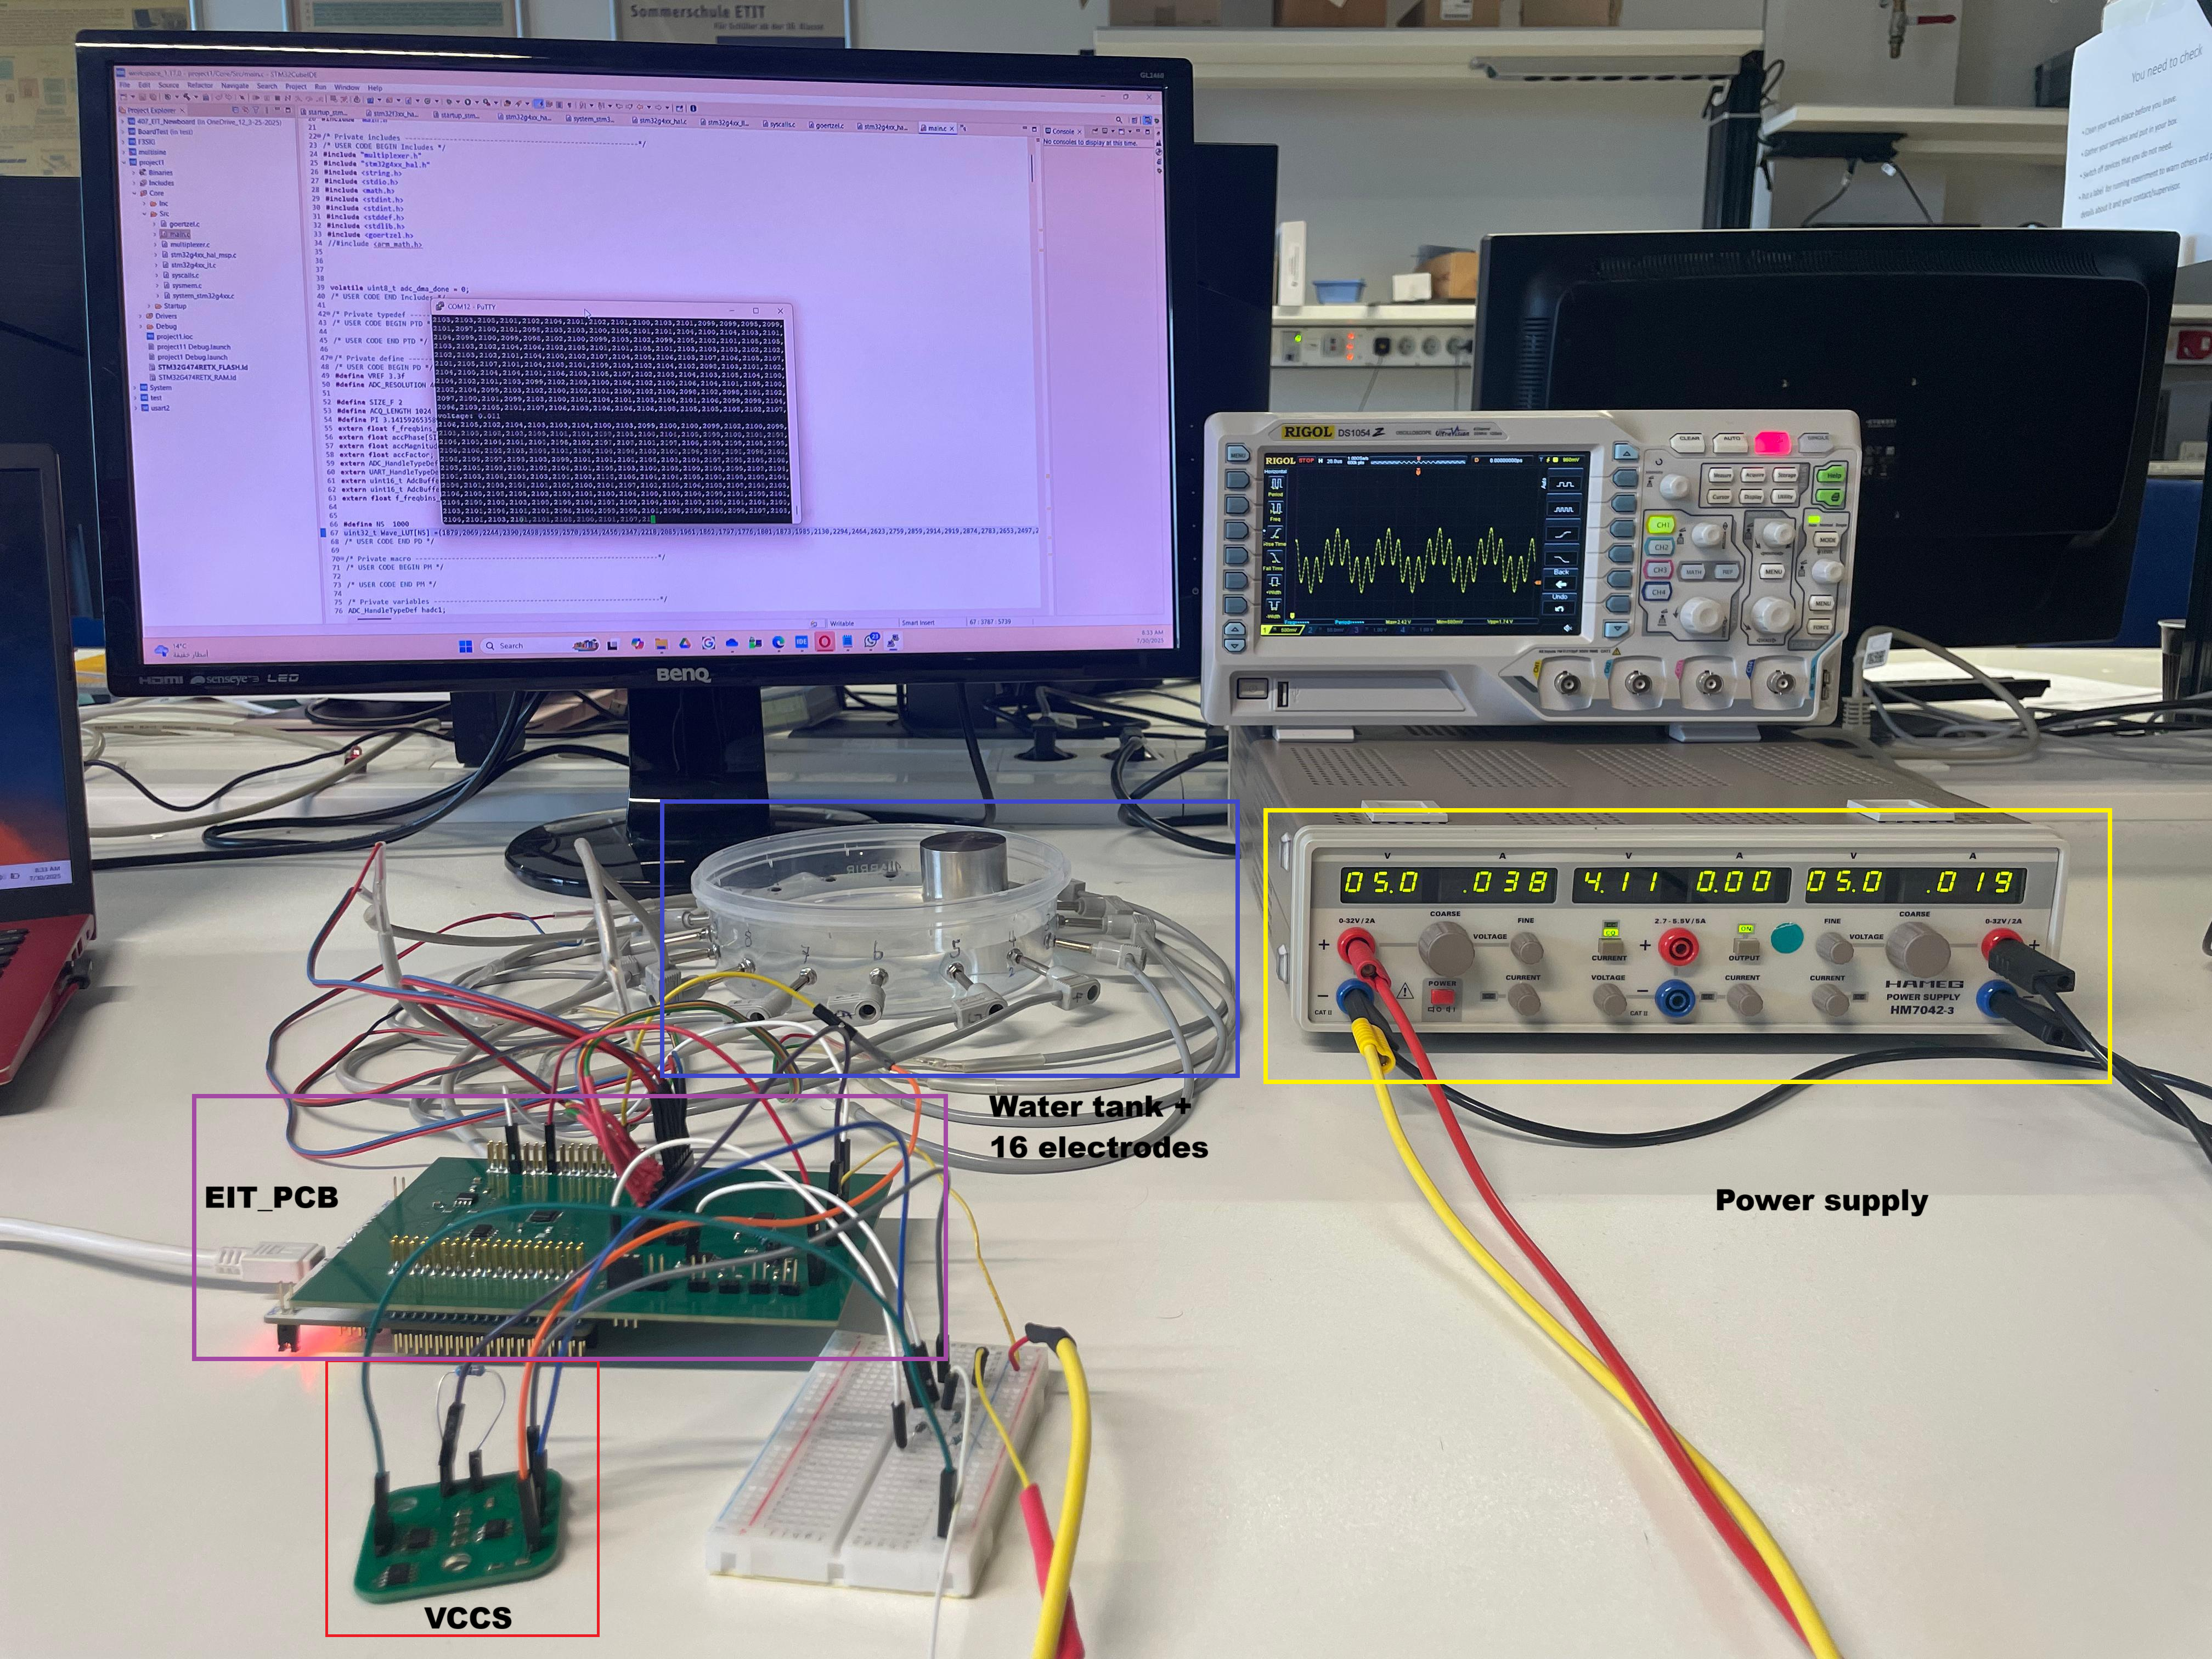
\includegraphics[width=0.95\textwidth]{imagess/setup.jpg}
    \caption{Experimental setup for system validation.}
    \label{fig:setup}
\end{figure}


\section{PCB testing and validation}
Before applying advanced signal processing and image reconstruction methods, it was essential to validate the designed PCB and ensure its correct functionality. The validation consisted of two main steps: (i) testing the circuit using a known resistance under monofrequency excitation, and (ii) testing the system with multi-frequency excitation using a water tank. These experiments demonstrate both the accuracy of the hardware and the robustness of the signal acquisition chain.  

\subsection{Validation with a known resistance}
To validate the analog front-end and switching architecture, the system was first tested by connecting a known resistor between two electrodes. A monofrequency sinusoidal excitation was injected by forcing the four multiplexers to select a pair of current-injection electrodes and a pair of voltage-sensing electrodes.  
 

The injected current and measured voltage were visualized on an oscilloscope. The calculated resistance, obtained from the ratio of measured voltage to current, closely matched the reference resistance value, confirming the accuracy of the measurement chain. Figure~\ref{fig:pcb_res_test} illustrates the oscilloscope visualization during this test.  

\begin{figure}[H]
    \centering
    \begin{subfigure}[b]{0.45\textwidth}
        \centering
        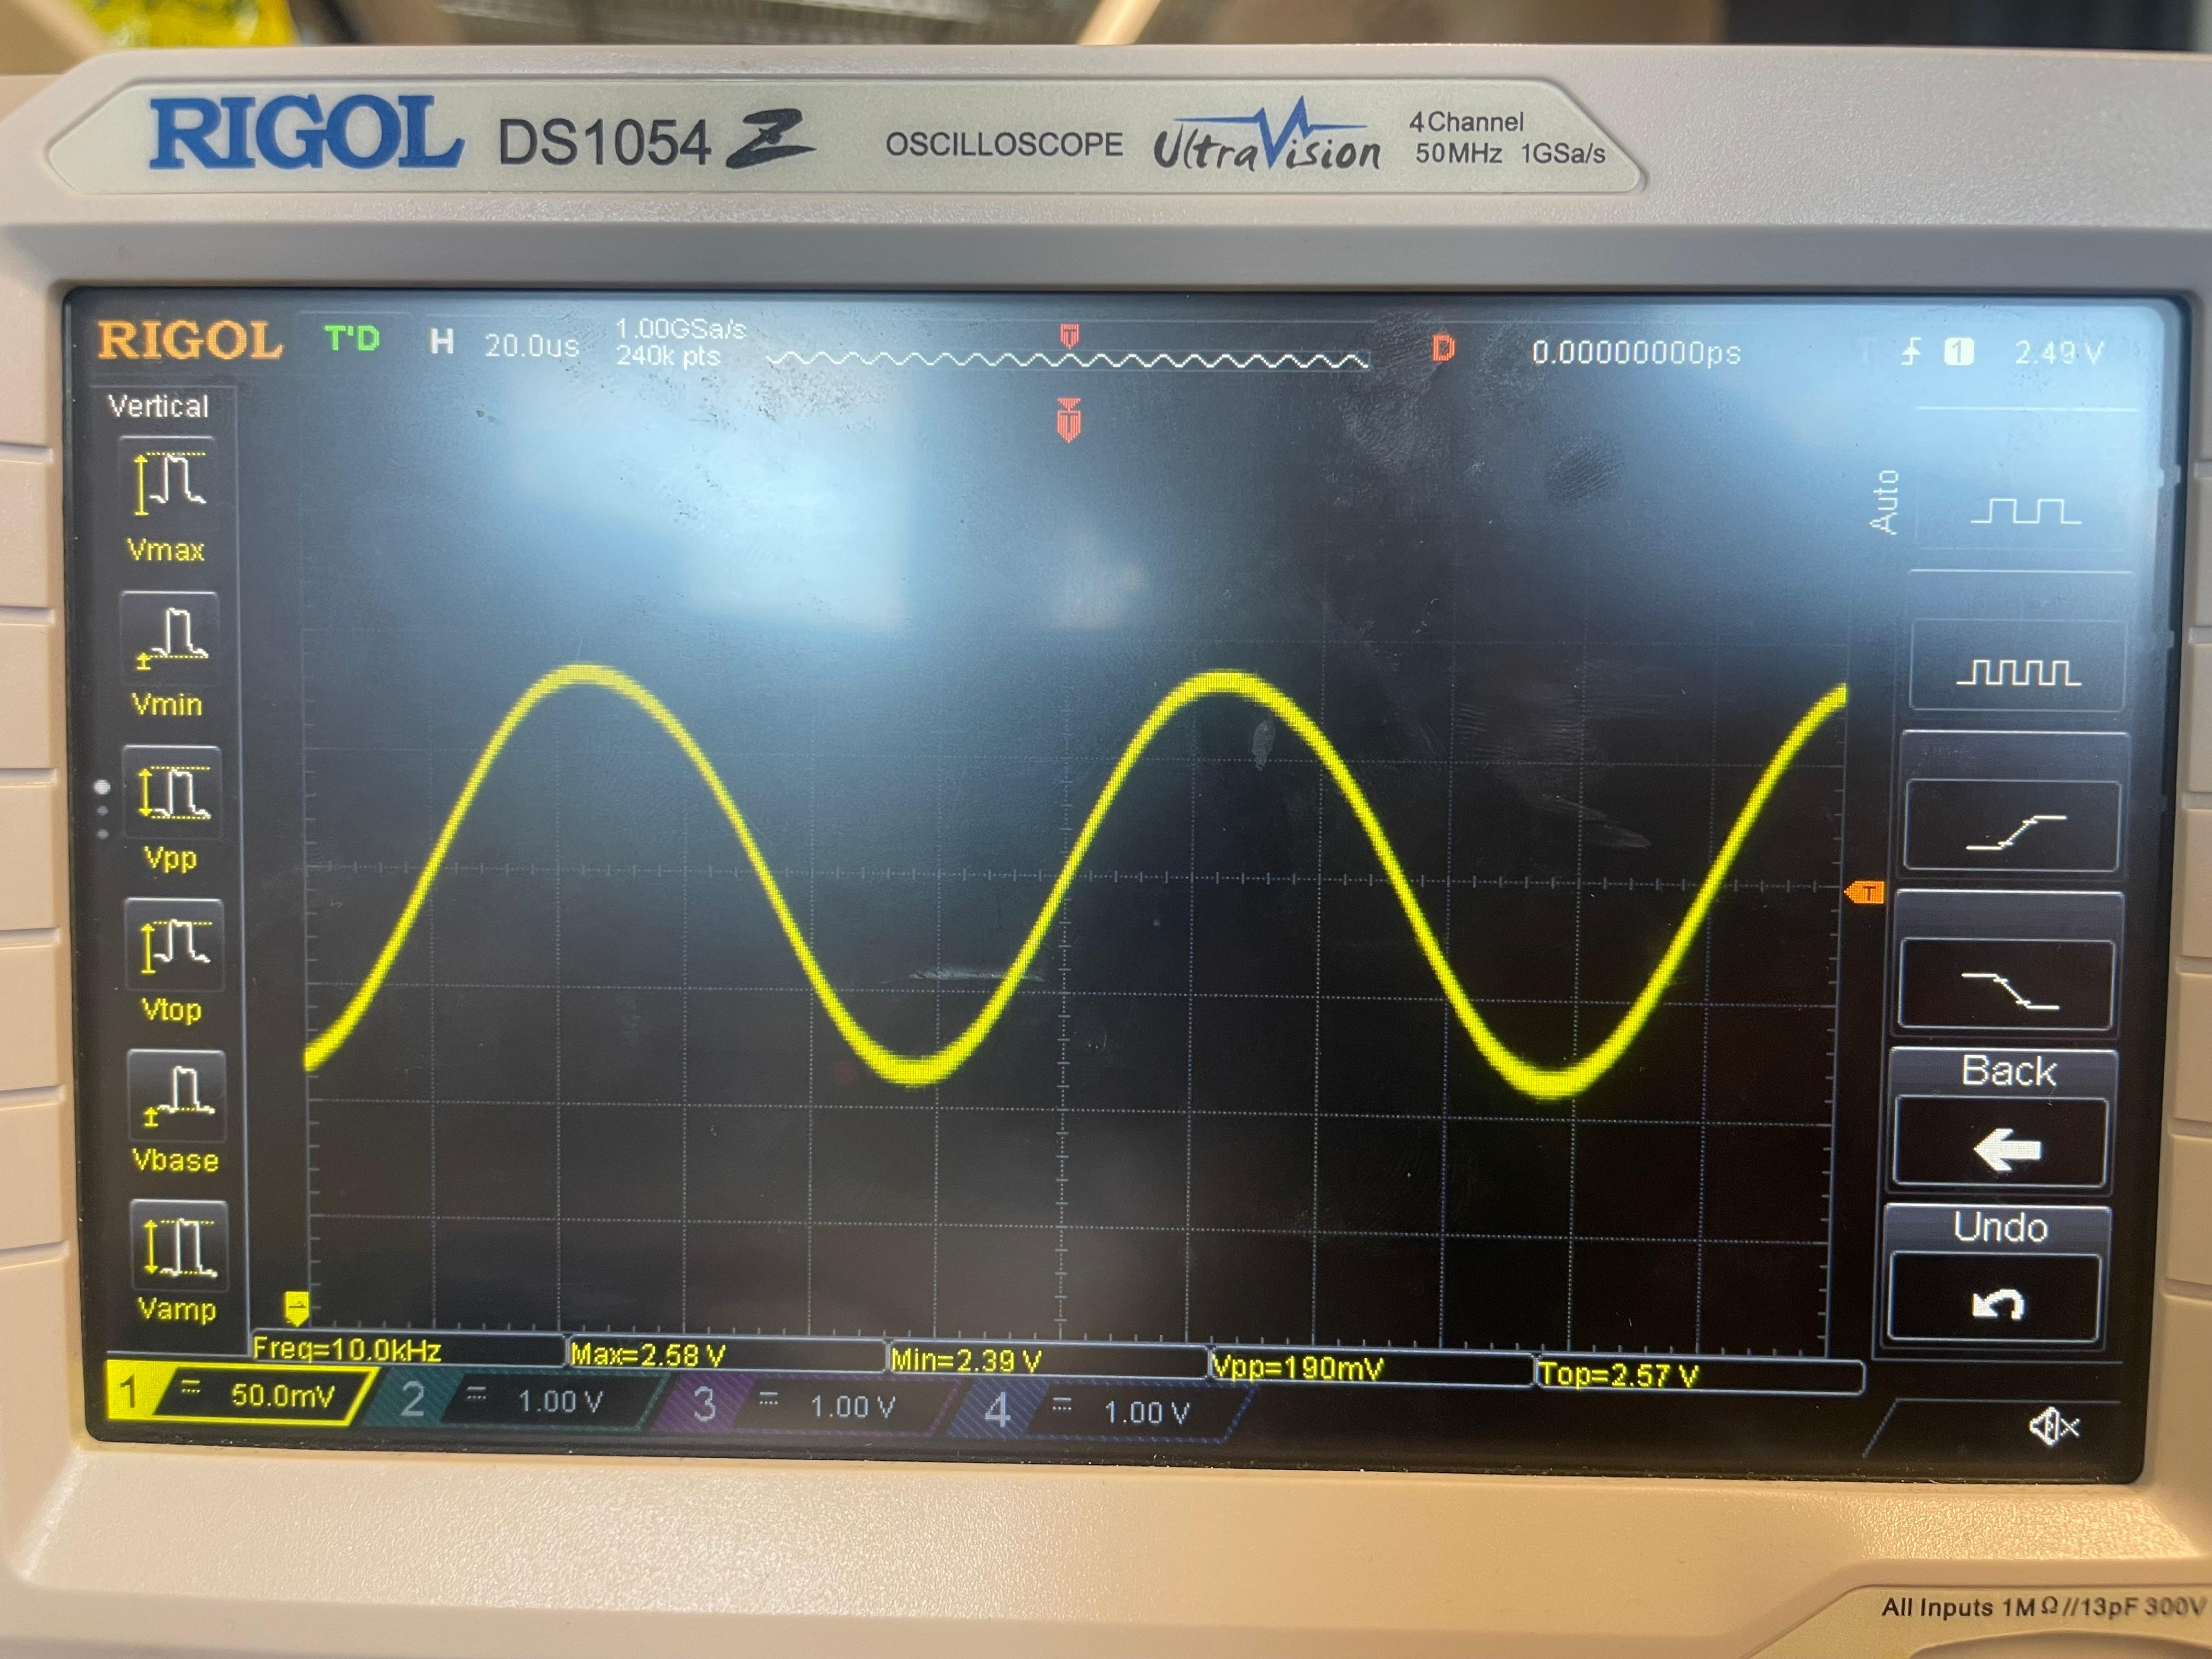
\includegraphics[width=\textwidth]{imagess/current.jpg}
        \caption{Measured current across a known resistance}
        \label{fig:current_test}
    \end{subfigure}
    \hfill
    \begin{subfigure}[b]{0.45\textwidth}
        \centering
        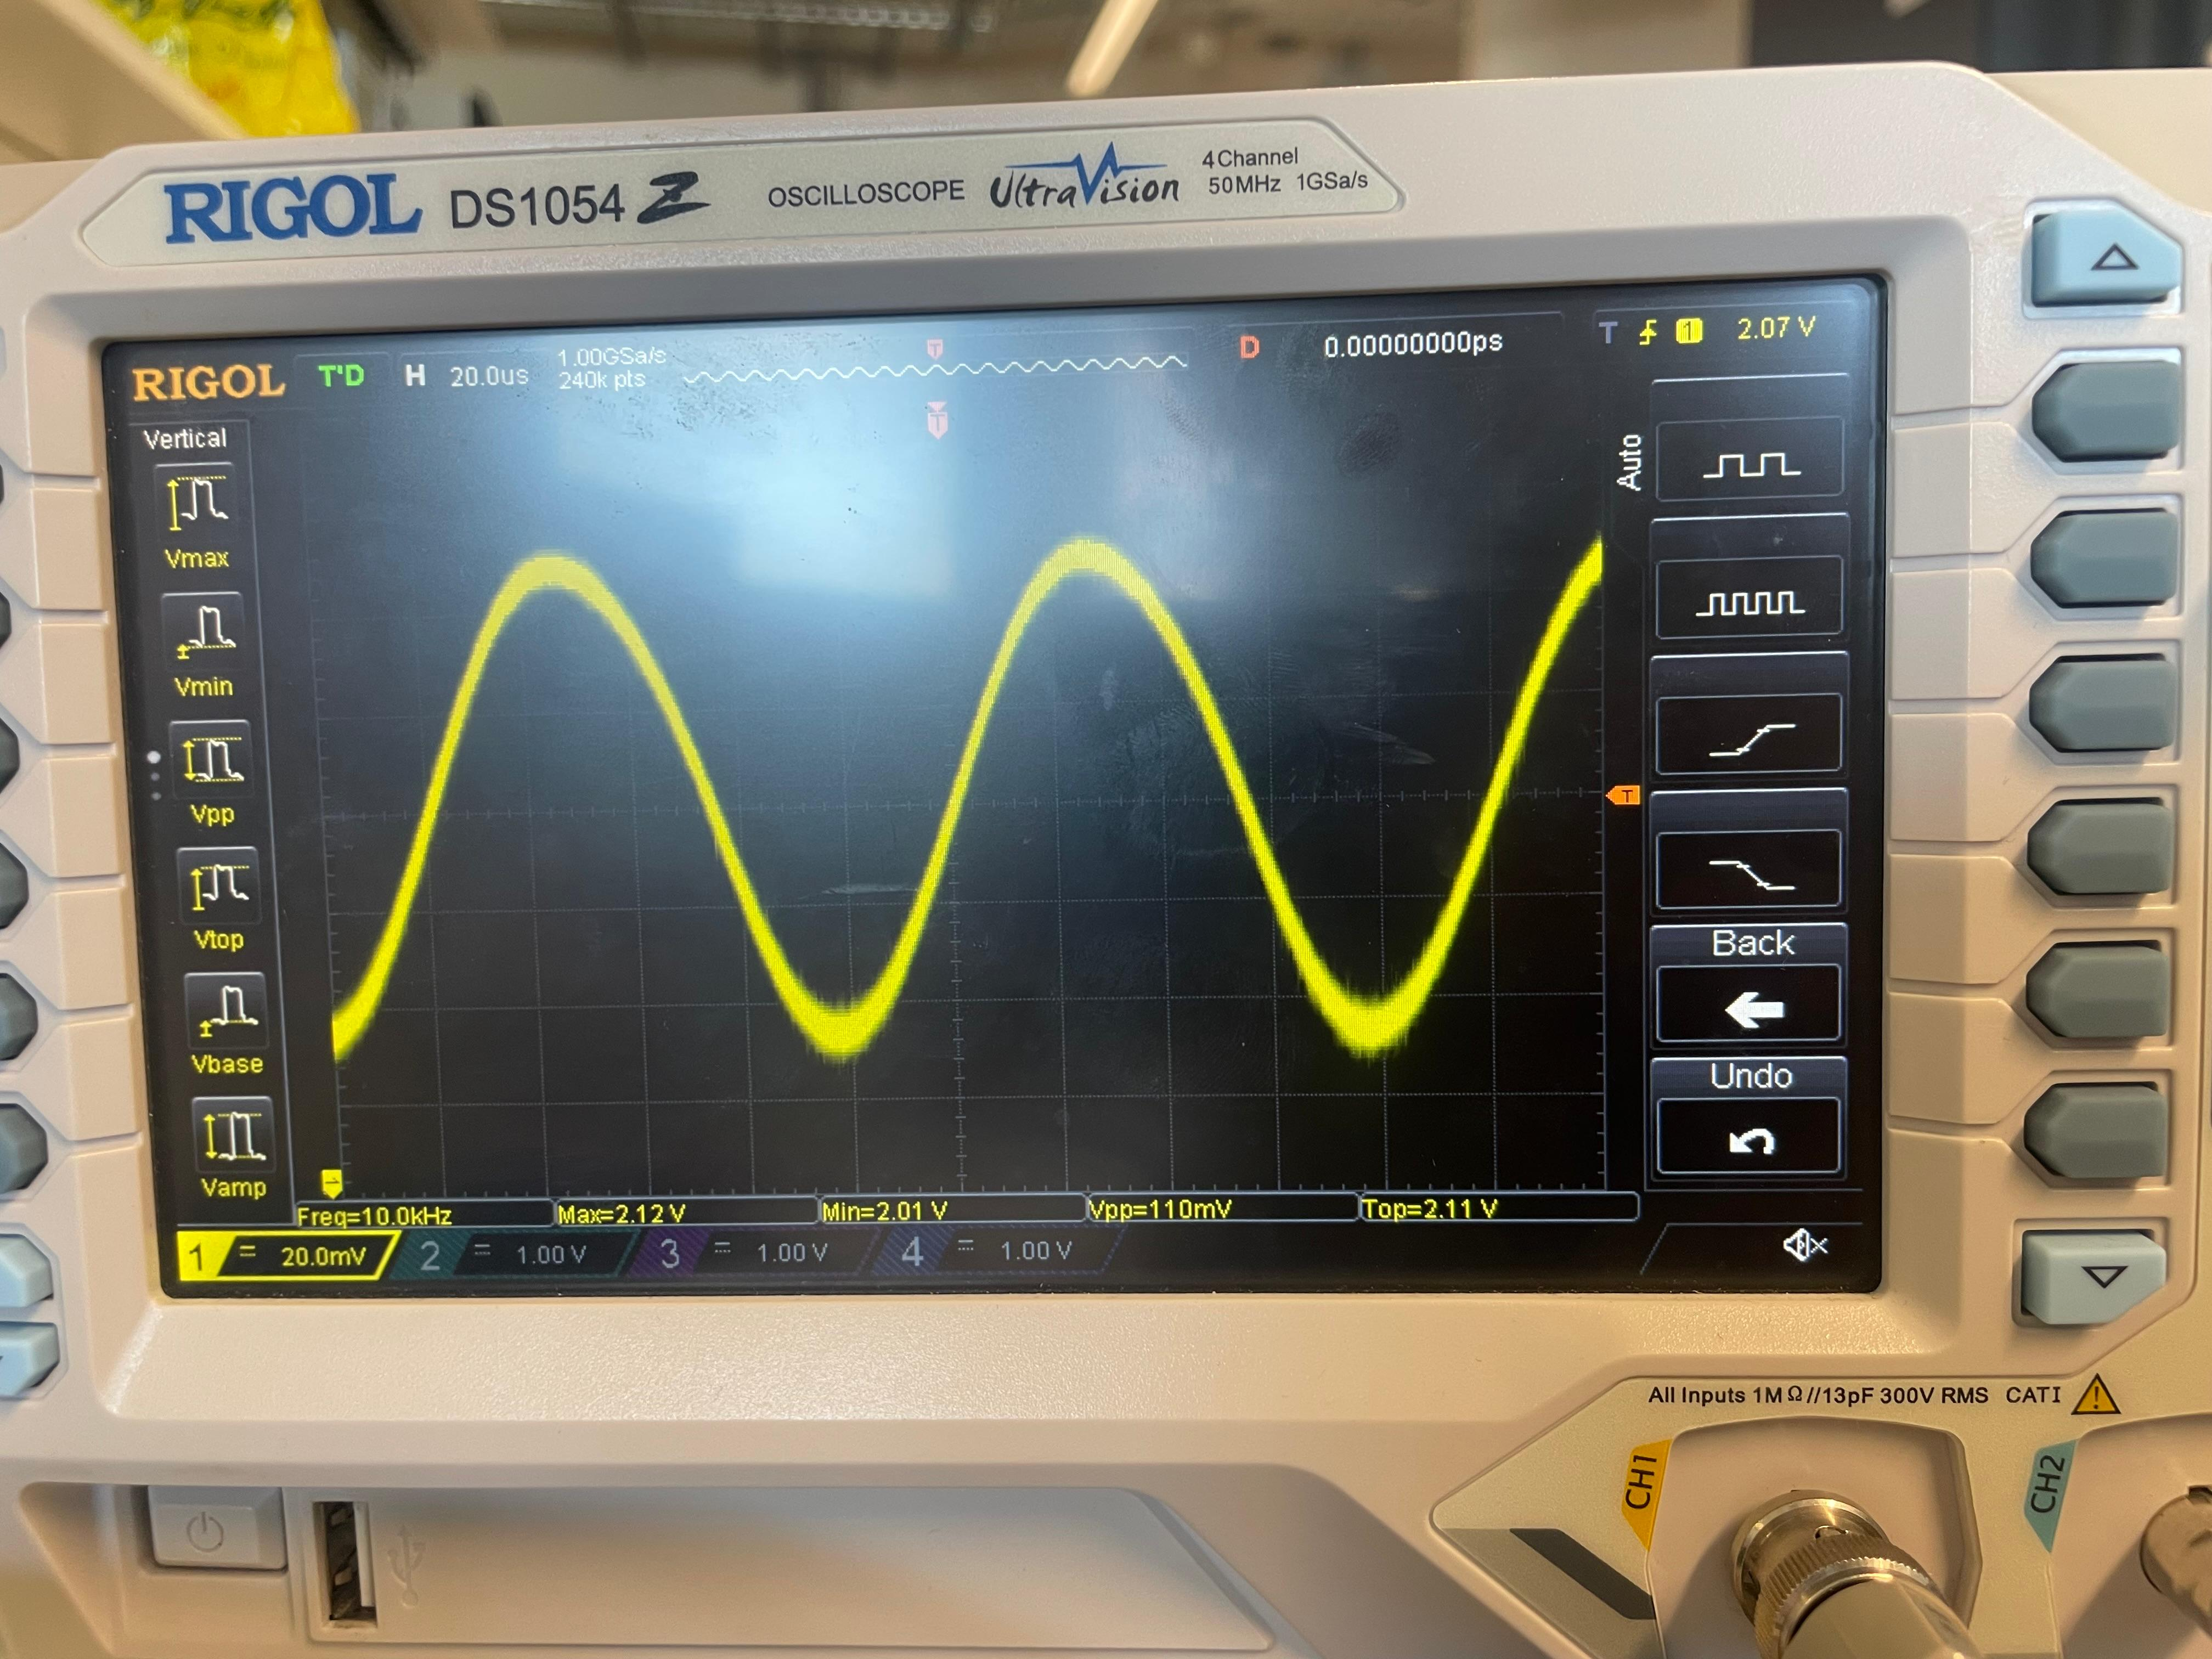
\includegraphics[width=\textwidth]{imagess/voltage.jpg}
        \caption{Measured voltage across a known resistance}
        \label{fig:voltage_test}
    \end{subfigure}
    \caption{Oscilloscope visualizations of the system response during a known resistance test.}
    \label{fig:pcb_res_test}
\end{figure}

Beyond qualitative waveform visualization, the system was quantitatively validated by extracting the peak-to-peak (V\textsubscript{pp}) values of the measured voltage and current signals from the oscilloscope traces.  

The procedure was as follows:  

\begin{itemize}

    \item The oscilloscope was used to measure the peak-to-peak voltage $V_{\text{pp,voltage}}$ across the load and the peak-to-peak voltage $V_{\text{pp,shunt}}$ across the current-sensing resistor $R_{\text{shunt}}$.
    \item The peak-to-peak current $I_{\text{pp}}$ was then calculated as:
    \begin{equation}
        I_{\text{pp}} = \frac{V_{\text{pp,shunt}}}{R_{\text{shunt}}}
    \end{equation}
    \item The load resistance $R_{\text{meas}}$ was obtained as:
    \begin{equation}
        R_{\text{meas}} = \frac{V_{\text{pp,voltage}}}{I_{\text{pp}}}
    \end{equation}
\end{itemize}

Table~\ref{tab:res_validation} summarizes the measured values compared with the true resistance ($\SI{1}{\kilo\ohm}$). The calculated resistance is in close agreement with the reference value, confirming the accuracy of the measurement chain.  

\begin{table}[H]
    \centering
    \caption{Oscilloscope-based validation of resistance measurement.}
    \label{tab:res_validation}
    \begin{tabular}{|c|c|c|c|c|}
        \hline
        $V_{\text{pp,voltage}}$ (mV) & $V_{\text{pp,shunt}}$ (mV) & $R_{\text{shunt}}$ ($\Omega$) & $I_{\text{pp}}$($\mu\text{A}$) & $R_{\text{meas}}$ ($\Omega$) \\
        \hline
       110 & 190 & 1000 & 190 & 578 \\
        \hline
    \end{tabular}
\end{table}
\subsection{Fabricated PCB after soldering}
After completing the design and fabrication process, the printed circuit board (PCB) was assembled by soldering all the required components.Figure~\ref{fig:pcb_after_soldering} shows the top side:

\begin{figure}[H]
    \centering
    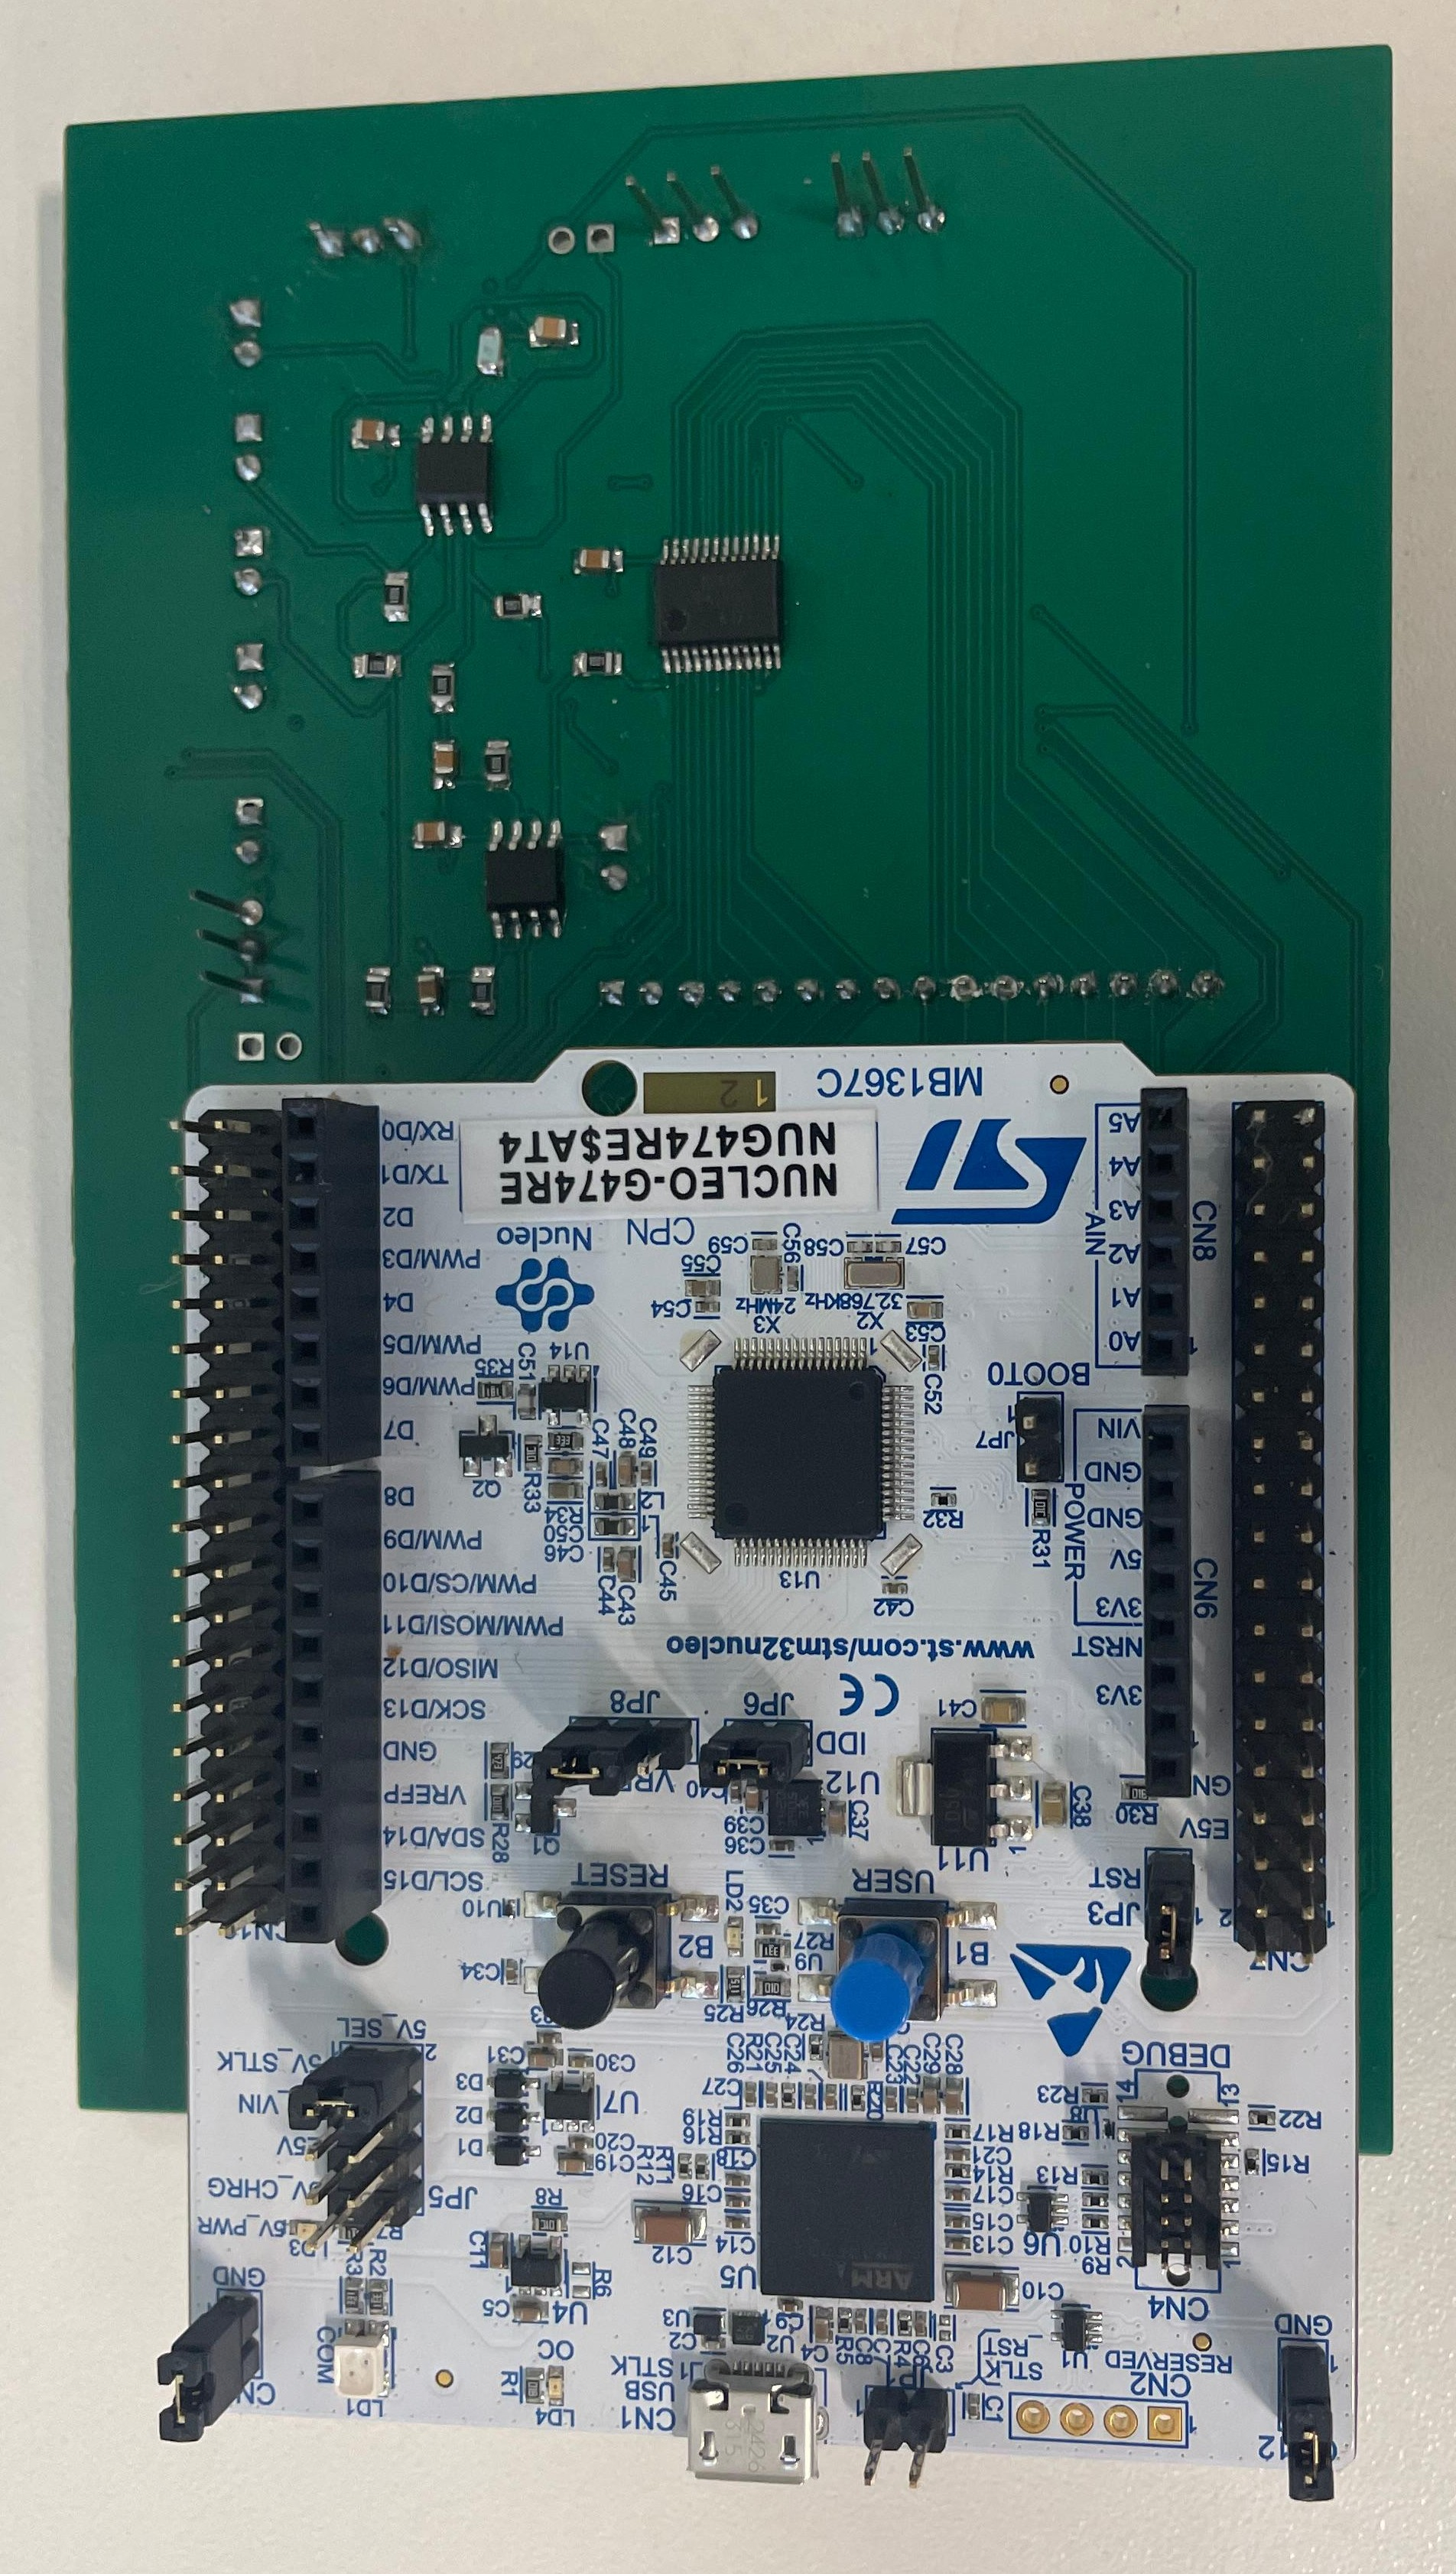
\includegraphics[width=0.65\textwidth]{imagess/top (1).jpg}
    \caption{Photograph of the fabricated PCB after soldering : top layer.}
    \label{fig:pcb_after_soldering}
\end{figure}
Figure~\ref{fig:pcb_after_soldering} shows the bottom side pf the PCB after soldering.
\begin{figure}[H]
    \centering
    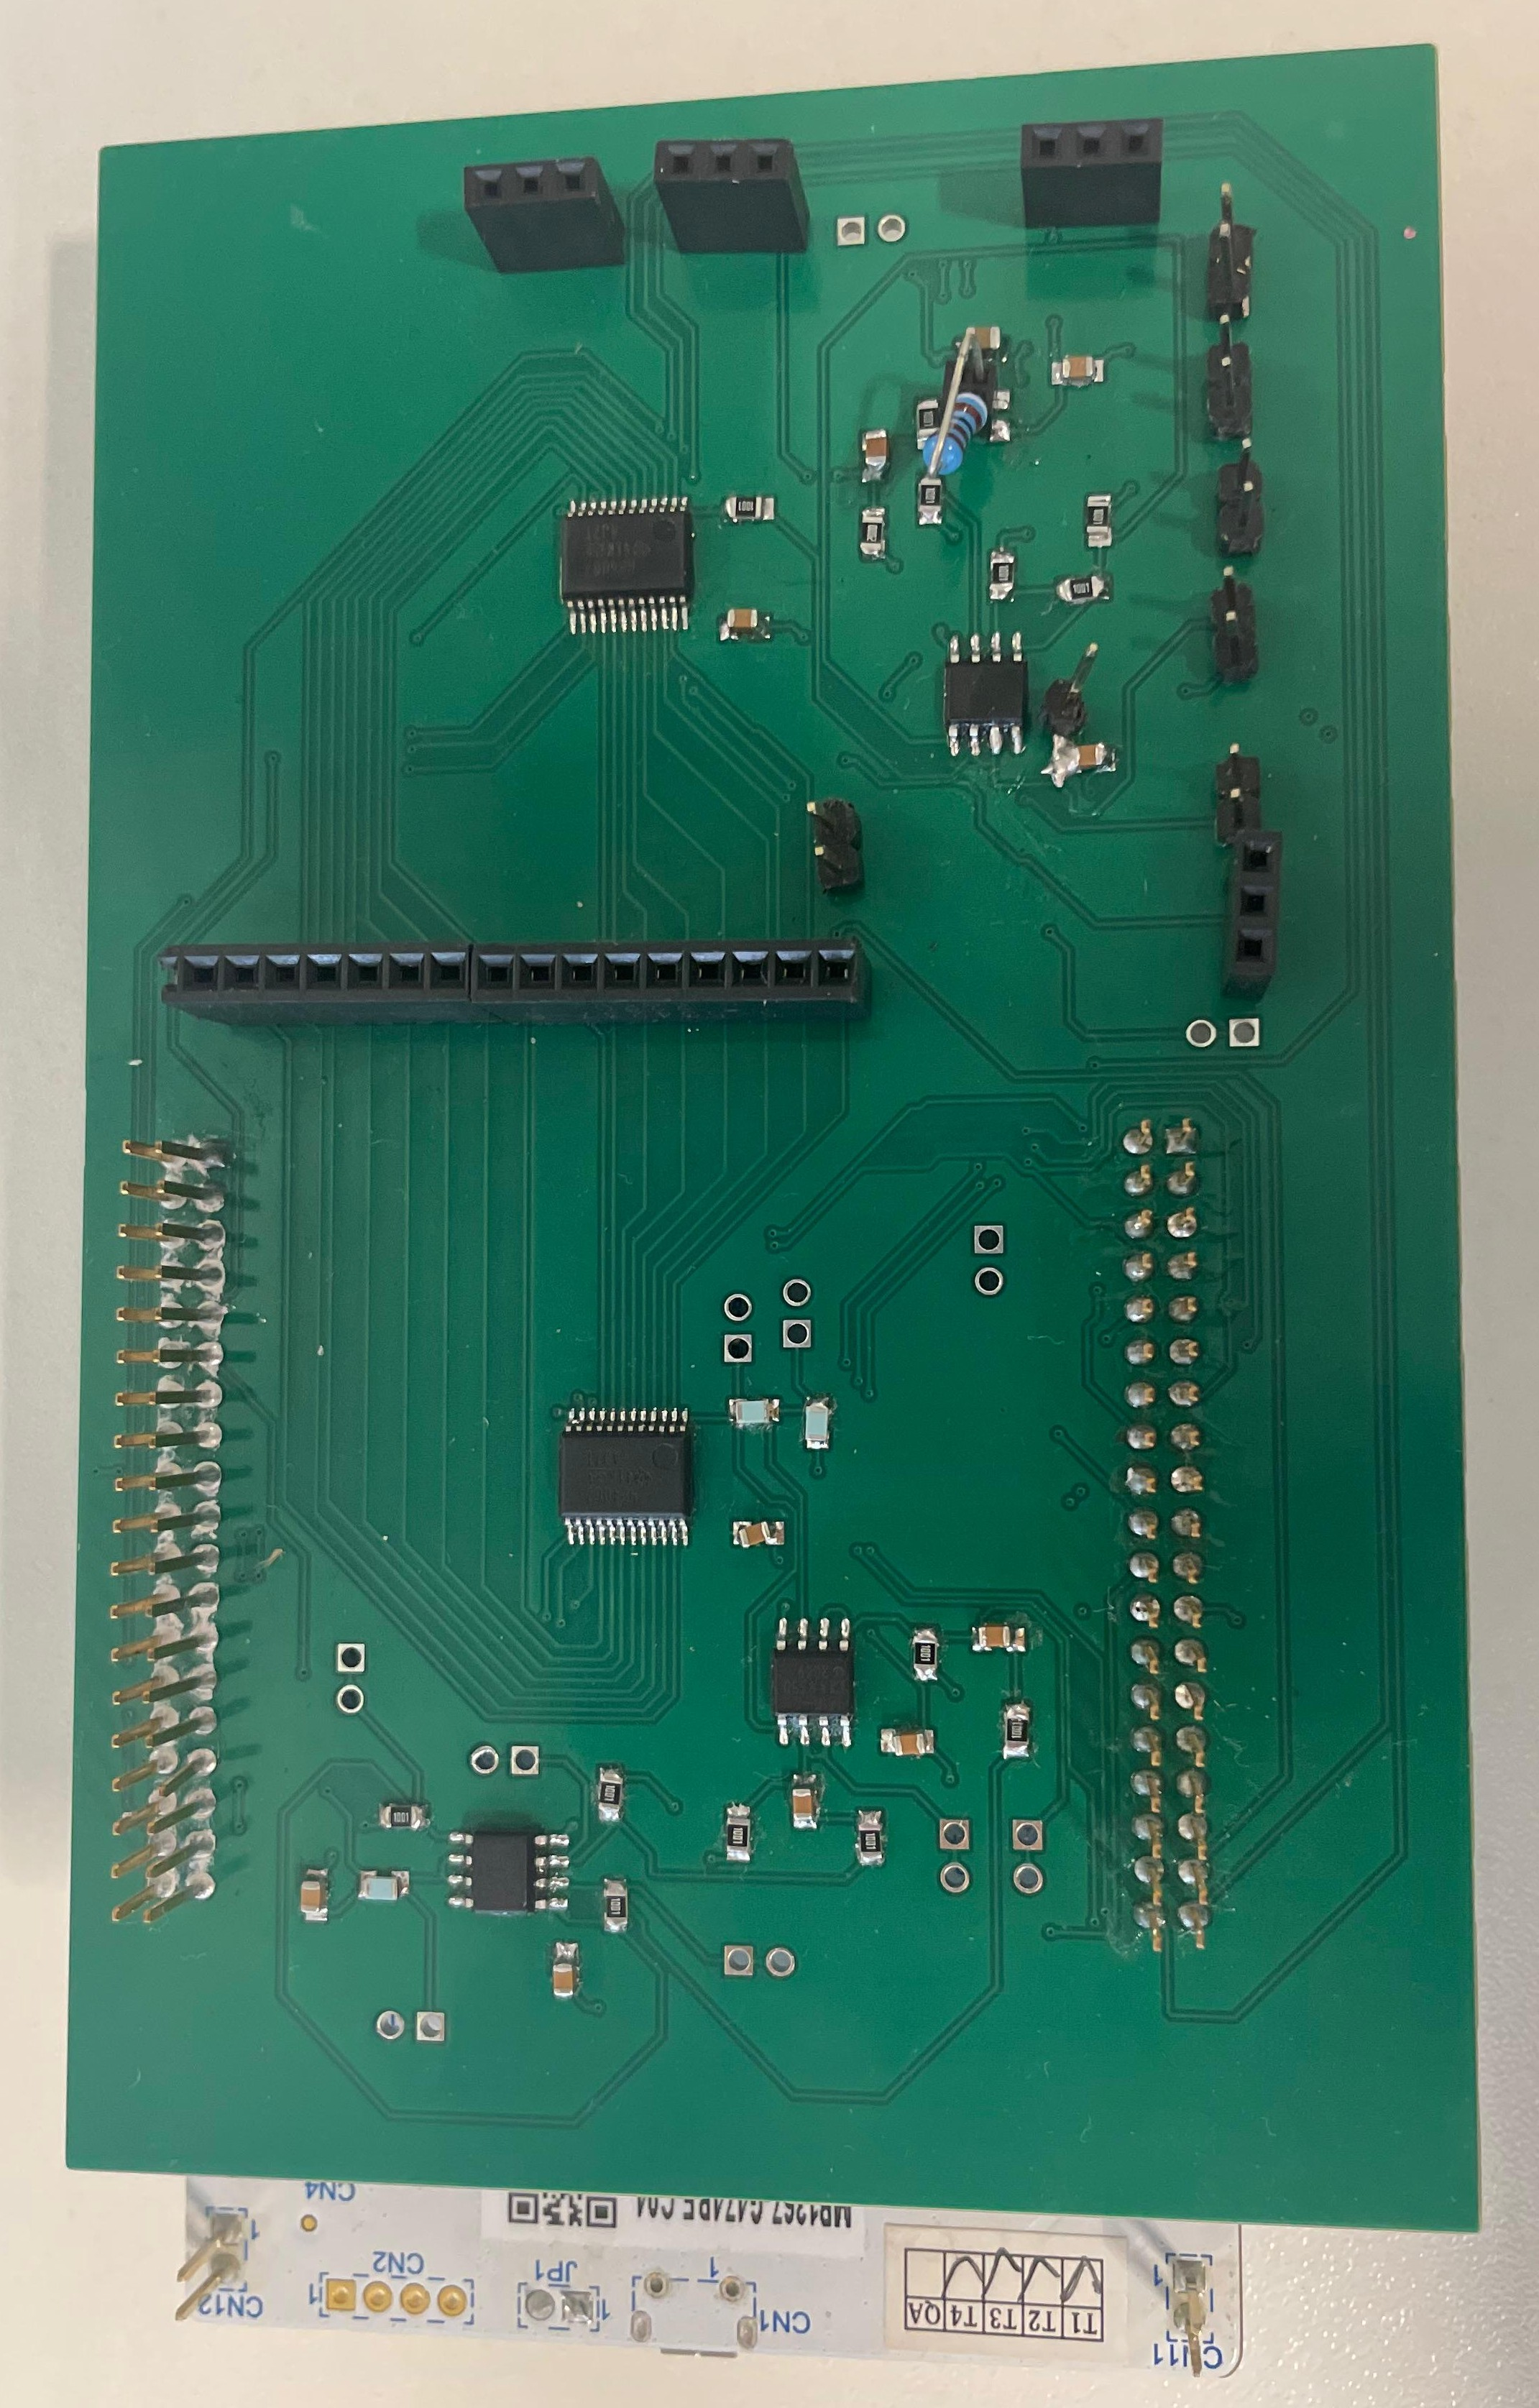
\includegraphics[width=0.65\textwidth]{imagess/bottom (1).jpg}
    \caption{Photograph of the fabricated PCB after soldering : bottom layer.}
    \label{fig:pcb_after_soldering}
\end{figure}

\section{Frequency-domain validation across 2 excitation frequencies}

To quantitatively validate the multi-frequency excitation, the system was tested with a known resistive load. 
The multiplexer was fixed to inject current between two electrodes and measure voltage between two others. 
The raw ADC samples were processed using both the Fast Fourier Transform (FFT) and the Goertzel algorithm implemented in Python. 
This allowed direct extraction of the magnitudes at the excitation frequencies (9.765 ~kHz and 49.804~kHz).

\subsection{FFT-based validation}
Figures~\ref{fig:fft_current} and \ref{fig:fft_voltage} present the FFT spectra of the injected current and measured voltage, respectively. 
Two distinct peaks are clearly visible at 9765~Hz and 49804~Hz, confirming that the multi-frequency excitation is correctly generated and acquired.

\begin{figure}[H]
    \centering
    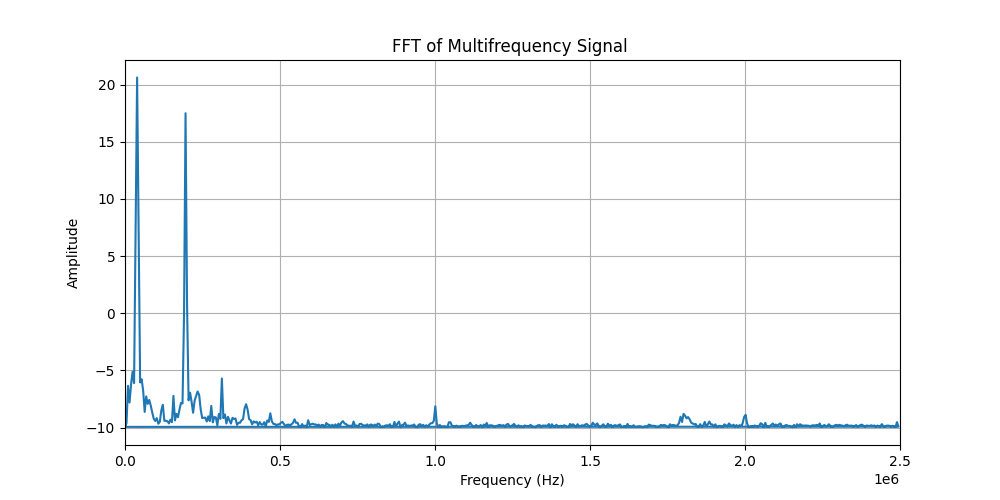
\includegraphics[width=0.85\textwidth]{imagess/Figure_current.png}
    \caption{FFT spectrum of the injected current showing distinct peaks at at $9765.6250$~Hz and   at $49804.6875$~Hz.}
    \label{fig:fft_current}
\end{figure}

\begin{figure}[H]
    \centering
    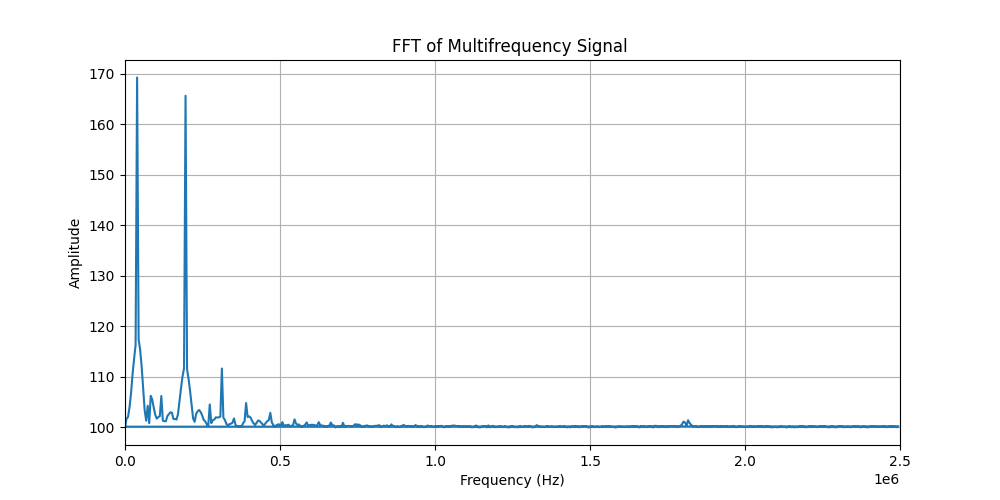
\includegraphics[width=0.85\textwidth]{imagess/fft2_measuredvoltage.png}
    \caption{FFT spectrum of the measured voltage showing distinct peaks at $9765.6250$~Hz and   at $49804.6875$~Hz.}
    \label{fig:fft_voltage}
\end{figure}

From the FFT magnitude values, the ADC peaks at $9765.6250$~Hz were found to be approximately:  
\[
V_{\text{measured}} \approx 170 \ \text{ADC counts}, 
\qquad V_{\text{shunt}} \approx 21 \ \text{ADC counts}.
\]

With a 12-bit ADC ($4096$ levels) and $V_{\mathrm{ref}}=3.3$~V, this corresponds to:
\[
V_{\mathrm{meas}}=\frac{170}{4096}\cdot 3.3 \approx 0.137~\text{V}, \qquad
V_{\mathrm{shunt}}=\frac{21}{4096}\cdot 3.3 \approx 0.0169~\text{V}.
\]

Using a shunt resistor of $R_{\mathrm{shunt}}=70~\Omega$, the injected current is:
\[
I = \frac{V_{\mathrm{shunt}}}{R_{\mathrm{shunt}}} = \frac{0.0169}{70} \approx 0.241~\text{mA}.
\]

The equivalent load resistance is therefore:
\[
R_{\mathrm{meas}} = \frac{V_{\mathrm{meas}}}{I} = \frac{0.137}{0.241\times 10^{-3}} \approx 568~\Omega,
\]
which is in good agreement with the true load value of $600~\Omega$.  
At $49804.6875$~Hz $R_{mes} = 637.995~\Omega$, confirming the frequency-independent behavior and the accuracy of the acquisition chain.

To further validate the results, the Goertzel algorithm was implemented in Python and applied to the same ADC datasets. 
The extracted magnitudes of voltage and current at 10~kHz and 50~kHz led to resistance values very close to those obtained with the FFT method. 
This demonstrates that both spectral techniques provide consistent and reliable results for impedance extraction in multi-frequency EIT.
\subsection{Quantitative evaluation of FFT-based validation}

To complement the qualitative observation of the FFT spectra, we quantified the accuracy of the impedance estimation at both excitation frequencies. The equivalent resistance was extracted from the ratio of measured voltage to current and compared to the known reference load of $600~\Omega$. The relative error was computed using:

\begin{equation}
\text{Error}(\%) = \frac{|R_{\text{measured}} - R_{\text{reference}}|}{R_{\text{reference}}} \times 100
\end{equation}

Table~\ref{tab:fft_eval} summarizes the results obtained with the FFT-based approach.

\begin{table}[H]
\centering
\caption{FFT-based resistance estimation and error analysis for two-frequency excitation}
\label{tab:fft_eval}
\begin{tabular}{|c|p{4cm}|p{4cm}|c|}
\hline
\textbf{Frequency (Hz)} & \textbf{Reference Resistance ($\Omega$)} & \textbf{Measured Resistance ($\Omega$)} & \textbf{Error (\%)} \\ \hline
9765.625  & 600 & 568   & 5.3  \\ \hline
49804.687 & 600 & 638   & 6.3  \\ \hline
\end{tabular}
\end{table}

The extracted resistance values closely match the true load, with errors below 7\%. This confirms that the proposed acquisition chain maintains reliable performance across both low and high excitation frequencies. 


\section{Validation of data acquisition and signal fidelity}
\label{sec:adc_validation}

Accurate acquisition of voltage measurements is a critical requirement for Electrical Impedance Tomography (EIT) systems. To ensure the reliability of the developed data acquisition system, the analog-to-digital converter (ADC) readings were validated using both mono- and multi-frequency excitation signals. This verification guarantees that the recorded impedance data accurately reflects the applied electrical stimuli, which is essential for subsequent tomographic reconstruction.

Figure~\ref{fig:adc_mono} shows the ADC readings obtained during a monofrequency excitation at 9.76 kHz. The acquired waveform closely follows the expected sinusoidal signal, indicating proper operation of the ADC and the signal conditioning circuitry.

\begin{figure}[H]
    \centering
    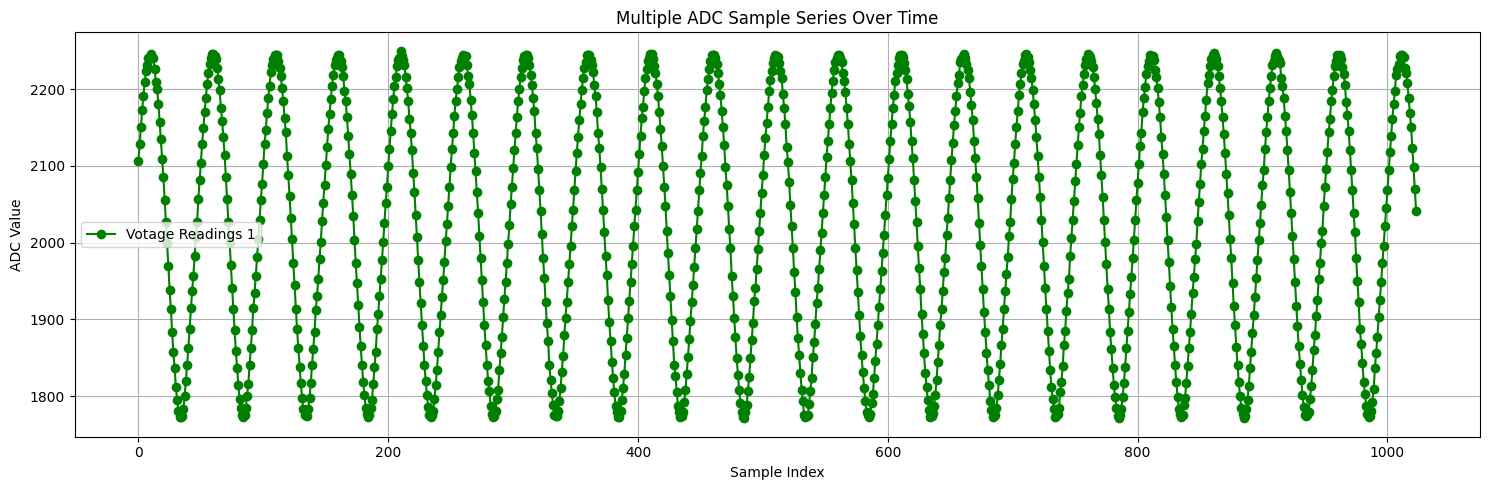
\includegraphics[width=0.8\textwidth]{imagess/s1.png}
    \caption{ADC readings for monofrequency excitation at 9.76 kHz. The waveform demonstrates accurate and stable sampling across multiple trials.}
    \label{fig:adc_mono}
\end{figure}

To further assess the system under realistic measurement conditions, multi-frequency excitation signals were applied, combining 9.76 kHz and 49.80 kHz components. Figure~\ref{fig:adc_multi} presents the corresponding ADC readings. The superimposed waveforms confirm that the ADC captures the composite signal with high fidelity, preserving both frequency components without noticeable distortion. This demonstrates that the system can reliably acquire data for multi-frequency EIT measurements, which are crucial for enhanced imaging sensitivity and resolution.

\begin{figure}[H]
    \centering
    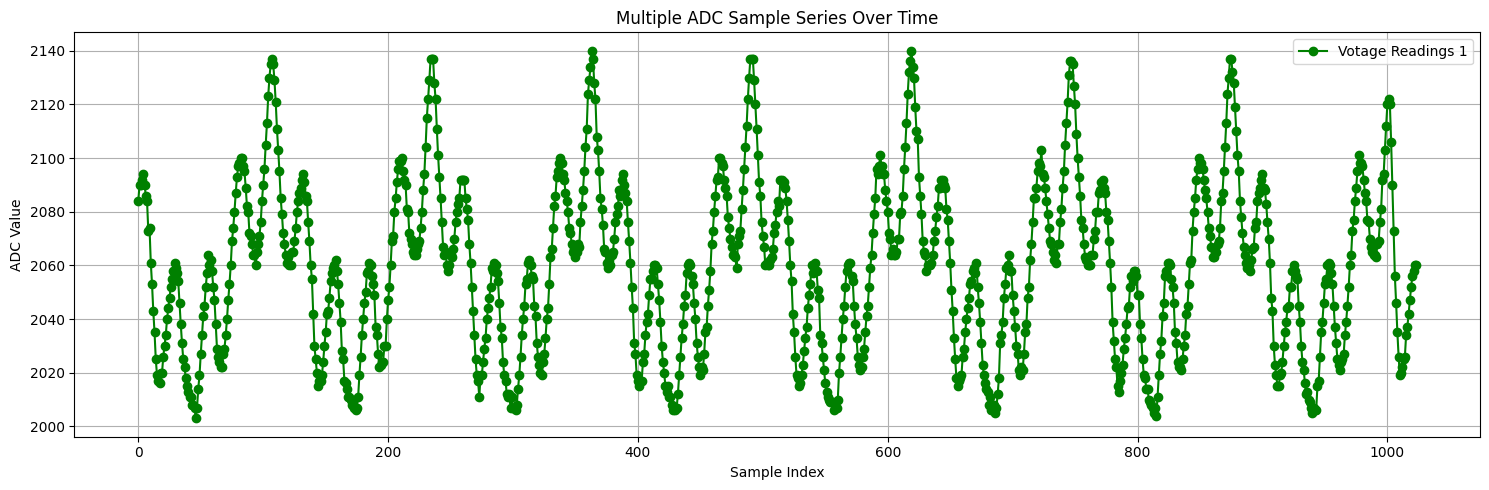
\includegraphics[width=0.8\textwidth]{imagess/s2.png}
    \caption{ADC readings for multi-frequency excitation at 9.76 kHz and 49.80 kHz. The ADC correctly resolves both frequency components, confirming signal fidelity.}
    \label{fig:adc_multi}
\end{figure}

The results from both monofrequency and multi-frequency validations confirm that the ADC and the associated acquisition pipeline provide accurate, stable, and repeatable measurements. These validations serve as a foundation for the reproducibility analyses presented in the next Sections.

\section{Measurement reproducibility across 2 excitation frequencies}
To ensure the reliability of the developed EIT acquisition system, it is important to
assess how consistently the measurements can be reproduced under repeated trials
and across different excitation frequencies. This section presents an experimental
evaluation of reproducibility, by comparing results at two representative
frequencies.
The following figures show the impedance variation over 20 trials for two different frequencies. The data was processed using a Python script that performs the following steps:

\begin{enumerate}
    \item Reads the raw EIT measurement data for each trial.
    \item Applies the Goertzel algorithm to extract the signal component at the frequency of interest.
    \item Computes the impedance values from the measured signals.

    \item Generates plots of the impedance variation across the 208 measurements for each trial.
\end{enumerate}

These steps allow visualizing how the impedance changes over repeated trials and between the two frequencies under study.

\begin{figure}[H]
    \centering
    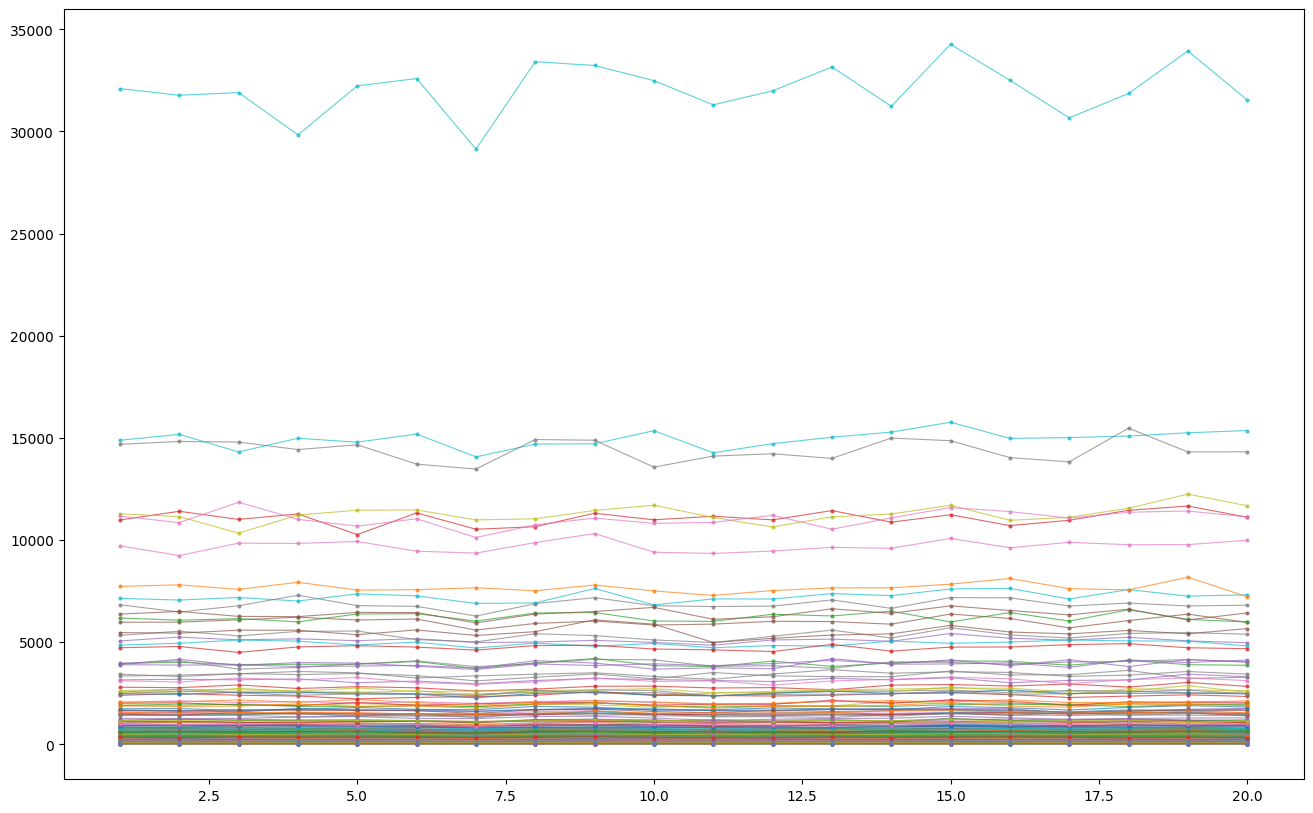
\includegraphics[width=0.7\textwidth]{imagess/2f_2.png}
    \caption{Impedance variation over 20 trials for \(f = 9765 \,\text{Hz}\) after Goertzel and impedance calculation.}
    \label{fig:stability_lowfreq}
\end{figure}

\begin{figure}[H]
    \centering
    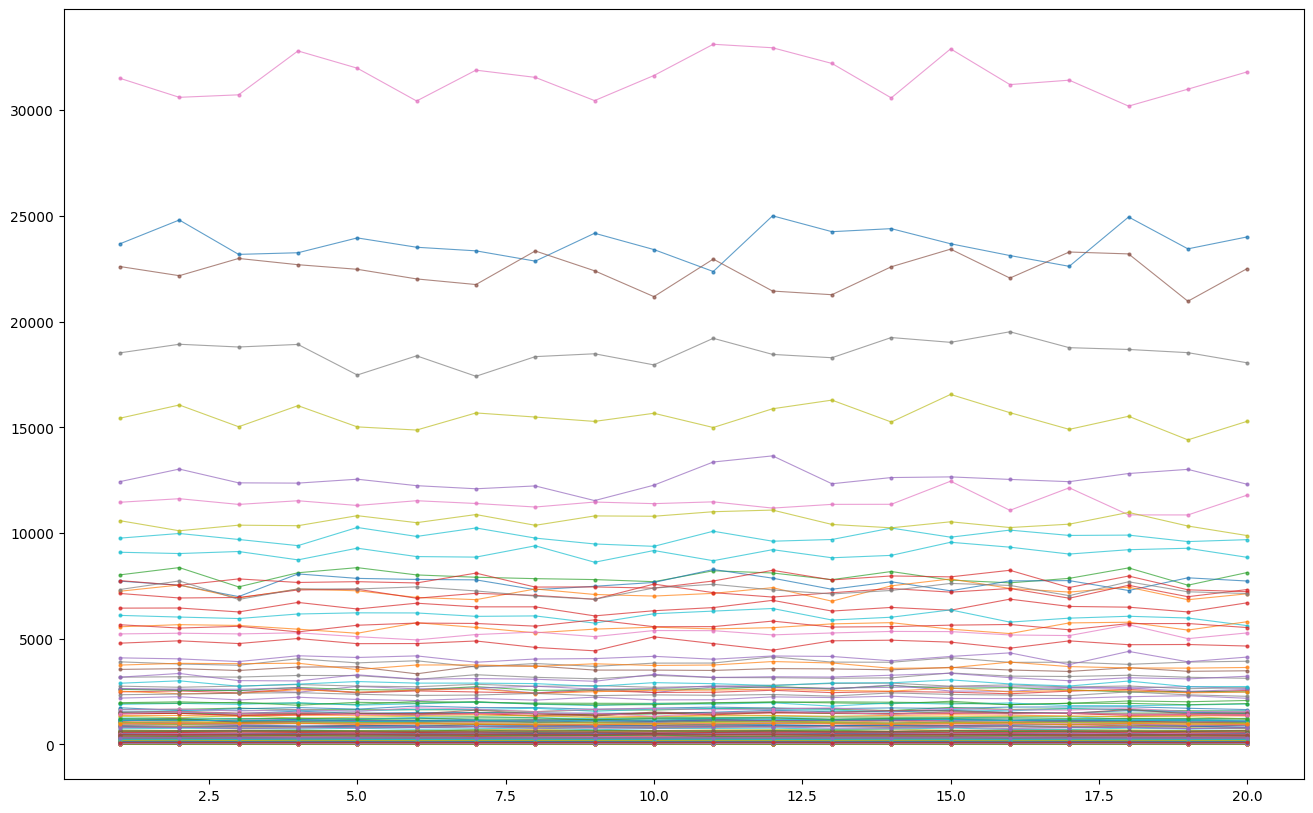
\includegraphics[width=0.7\textwidth]{imagess/2f_1.png}
    \caption{Impedance variation over 20 trials for \(f = 49804 \,\text{Hz}\) after Goertzel and impedance calculation.}
    \label{fig:stability_highfreq}
\end{figure}

The impedance results presented in Figures~\ref{fig:stability_lowfreq} and 
\ref{fig:stability_highfreq} confirm the robustness of the measurement system. 
For the lower frequency case (\(f = 9765 \,\text{Hz}\)), the impedance values 
remain highly stable across the 20 trials, with only minor fluctuations. 
This demonstrates that the system maintains a consistent response under 
repeated measurements.

At the higher frequency (\(f = 49804 \,\text{Hz}\)), the impedance curves 
exhibit slightly larger variations between trials, which can be attributed 
to increased sensitivity of the measurement to electrode-skin interface 
changes and parasitic effects at higher frequencies. Nevertheless, the 
overall trends remain consistent, indicating that the system does not suffer 
from long-term drift or instability.

These results confirm that the developed EIT acquisition system provides 
reproducible impedance measurements across multiple trials and under 
different frequency conditions, which is crucial for reliable tomographic 
reconstruction.



\section{Multi-frequency experimental validation using image reconstruction}
In order to evaluate the capability of the developed multi-frequency EIT system,
We performed test-tank experiments with a metallic cylindrical object combined with conductivity image
reconstruction. This section first outlines the reconstruction algorithm employed
for processing the measurement data and then presents experimental validations
across two and five excitation frequencies, highlighting the quality and
limitations of the reconstructed images.

\subsection{Image reconstruction algorithm}

To obtain conductivity distribution images from the multi-frequency EIT system, we employed an image reconstruction algorithm based on the \textbf{Jacobian (JAC) method} with the \textbf{Gauss--Newton optimization scheme}. The following steps summarize the reconstruction workflow:

\begin{enumerate}
    \item \textbf{Forward model and protocol setup} \\
    The EIT system is modeled using a finite element mesh of the imaging domain, which includes the electrode positions and background conductivity distribution. A stimulation protocol is defined (\texttt{protocol.create(16)}), where 16 electrodes are placed around the boundary and adjacent current injections with voltage measurements are specified.

    \item \textbf{Jacobian-based inverse solver (JAC)} \\
    The inverse problem in EIT aims to recover the internal conductivity distribution from boundary voltage measurements. We use the \texttt{jac.JAC} solver, which linearizes the relationship between conductivity changes and measured voltages.  
    \begin{itemize}
        \item The Jacobian matrix describes the sensitivity of voltage measurements to conductivity perturbations inside the domain.
        \item A regularization term is included to stabilize the inversion, with parameters $p = 0.01$ (prior weight) and $\lambda = 10^{-4}$ (Tikhonov regularization).
        \item The \emph{Kotre method} is applied as the reconstruction strategy, which is well-suited for difference EIT.
    \end{itemize}

    \item \textbf{Measurement data acquisition} \\
    Two measurement datasets are considered:
    \begin{itemize}
        \item \texttt{water\_new\_hardware}: reference dataset measured with the imaging domain filled with homogeneous water (baseline).
        \item \texttt{object\_new\_hardware}: dataset measured when a conductive object is introduced into the water tank.
    \end{itemize}

    \item \textbf{Gauss--Newton iterative reconstruction} \\
    Using the Gauss--Newton algorithm (\texttt{eit.gn}), the conductivity distribution is updated iteratively by minimizing the difference between measured and simulated voltages. Only one iteration (\texttt{maxiter=1}) is applied here, since we focus on difference imaging rather than absolute conductivity mapping.

    \item \textbf{Difference imaging} \\
    To highlight only the object, a difference image is computed:
    \[
        \Delta \sigma = \sigma_{\text{water}} - \sigma_{\text{object}}
    \]
    This cancels out the homogeneous background and emphasizes the perturbation caused by the inserted object.

    \item \textbf{Normalization} \\
    The reconstructed conductivity changes are normalized to the range $[0, 1]$:
    \[
        \sigma_{\text{norm}} = \frac{\sigma - \sigma_{\min}}{\sigma_{\max} - \sigma_{\min}}
    \]
    This ensures consistent visualization independent of the raw measurement scale.

    \item \textbf{Image visualization} \\
    The normalized conductivity changes are mapped onto the mesh using triangular interpolation (\texttt{ax.tripcolor}). Electrode positions are overlaid on the reconstructed image to indicate measurement points.
\end{enumerate}

This approach provides a \textbf{difference EIT reconstruction} that suppresses common-mode artifacts (from electrode contact impedance, system drift, etc.) and enhances the visibility of localized conductivity changes due to the introduced object.

\subsection{Experimental validation across 2 excitation frequencies}

To validate the system performance in a realistic scenario, a water tank with metallic cylinder was used as an experimental setup. Two multi-frequency excitations were injected simultaneously; for a multi-frequency excitation signal corresponding to two frequencies: $9765$ Hz and $49804$ Hz. The reconstructed images at two different positions for each frequency are displayed in the figures below.

Two cases were studied:
\begin{itemize}
    \item A metallic object positioned near electrode~0.
    \item The same object repositioned near electrode~7.
\end{itemize}
% Explanatory sentence before the figure
The real water tank setup with the metallic cylindrical object is shown below for two different positions: near electrode 0 (left) and near electrode 7 (right). This serves as a reference for the reconstructed conductivity maps.

\begin{figure}[H]
    \centering
    % Subfigure for position near electrode 0
    \begin{subfigure}[b]{0.32\linewidth}
        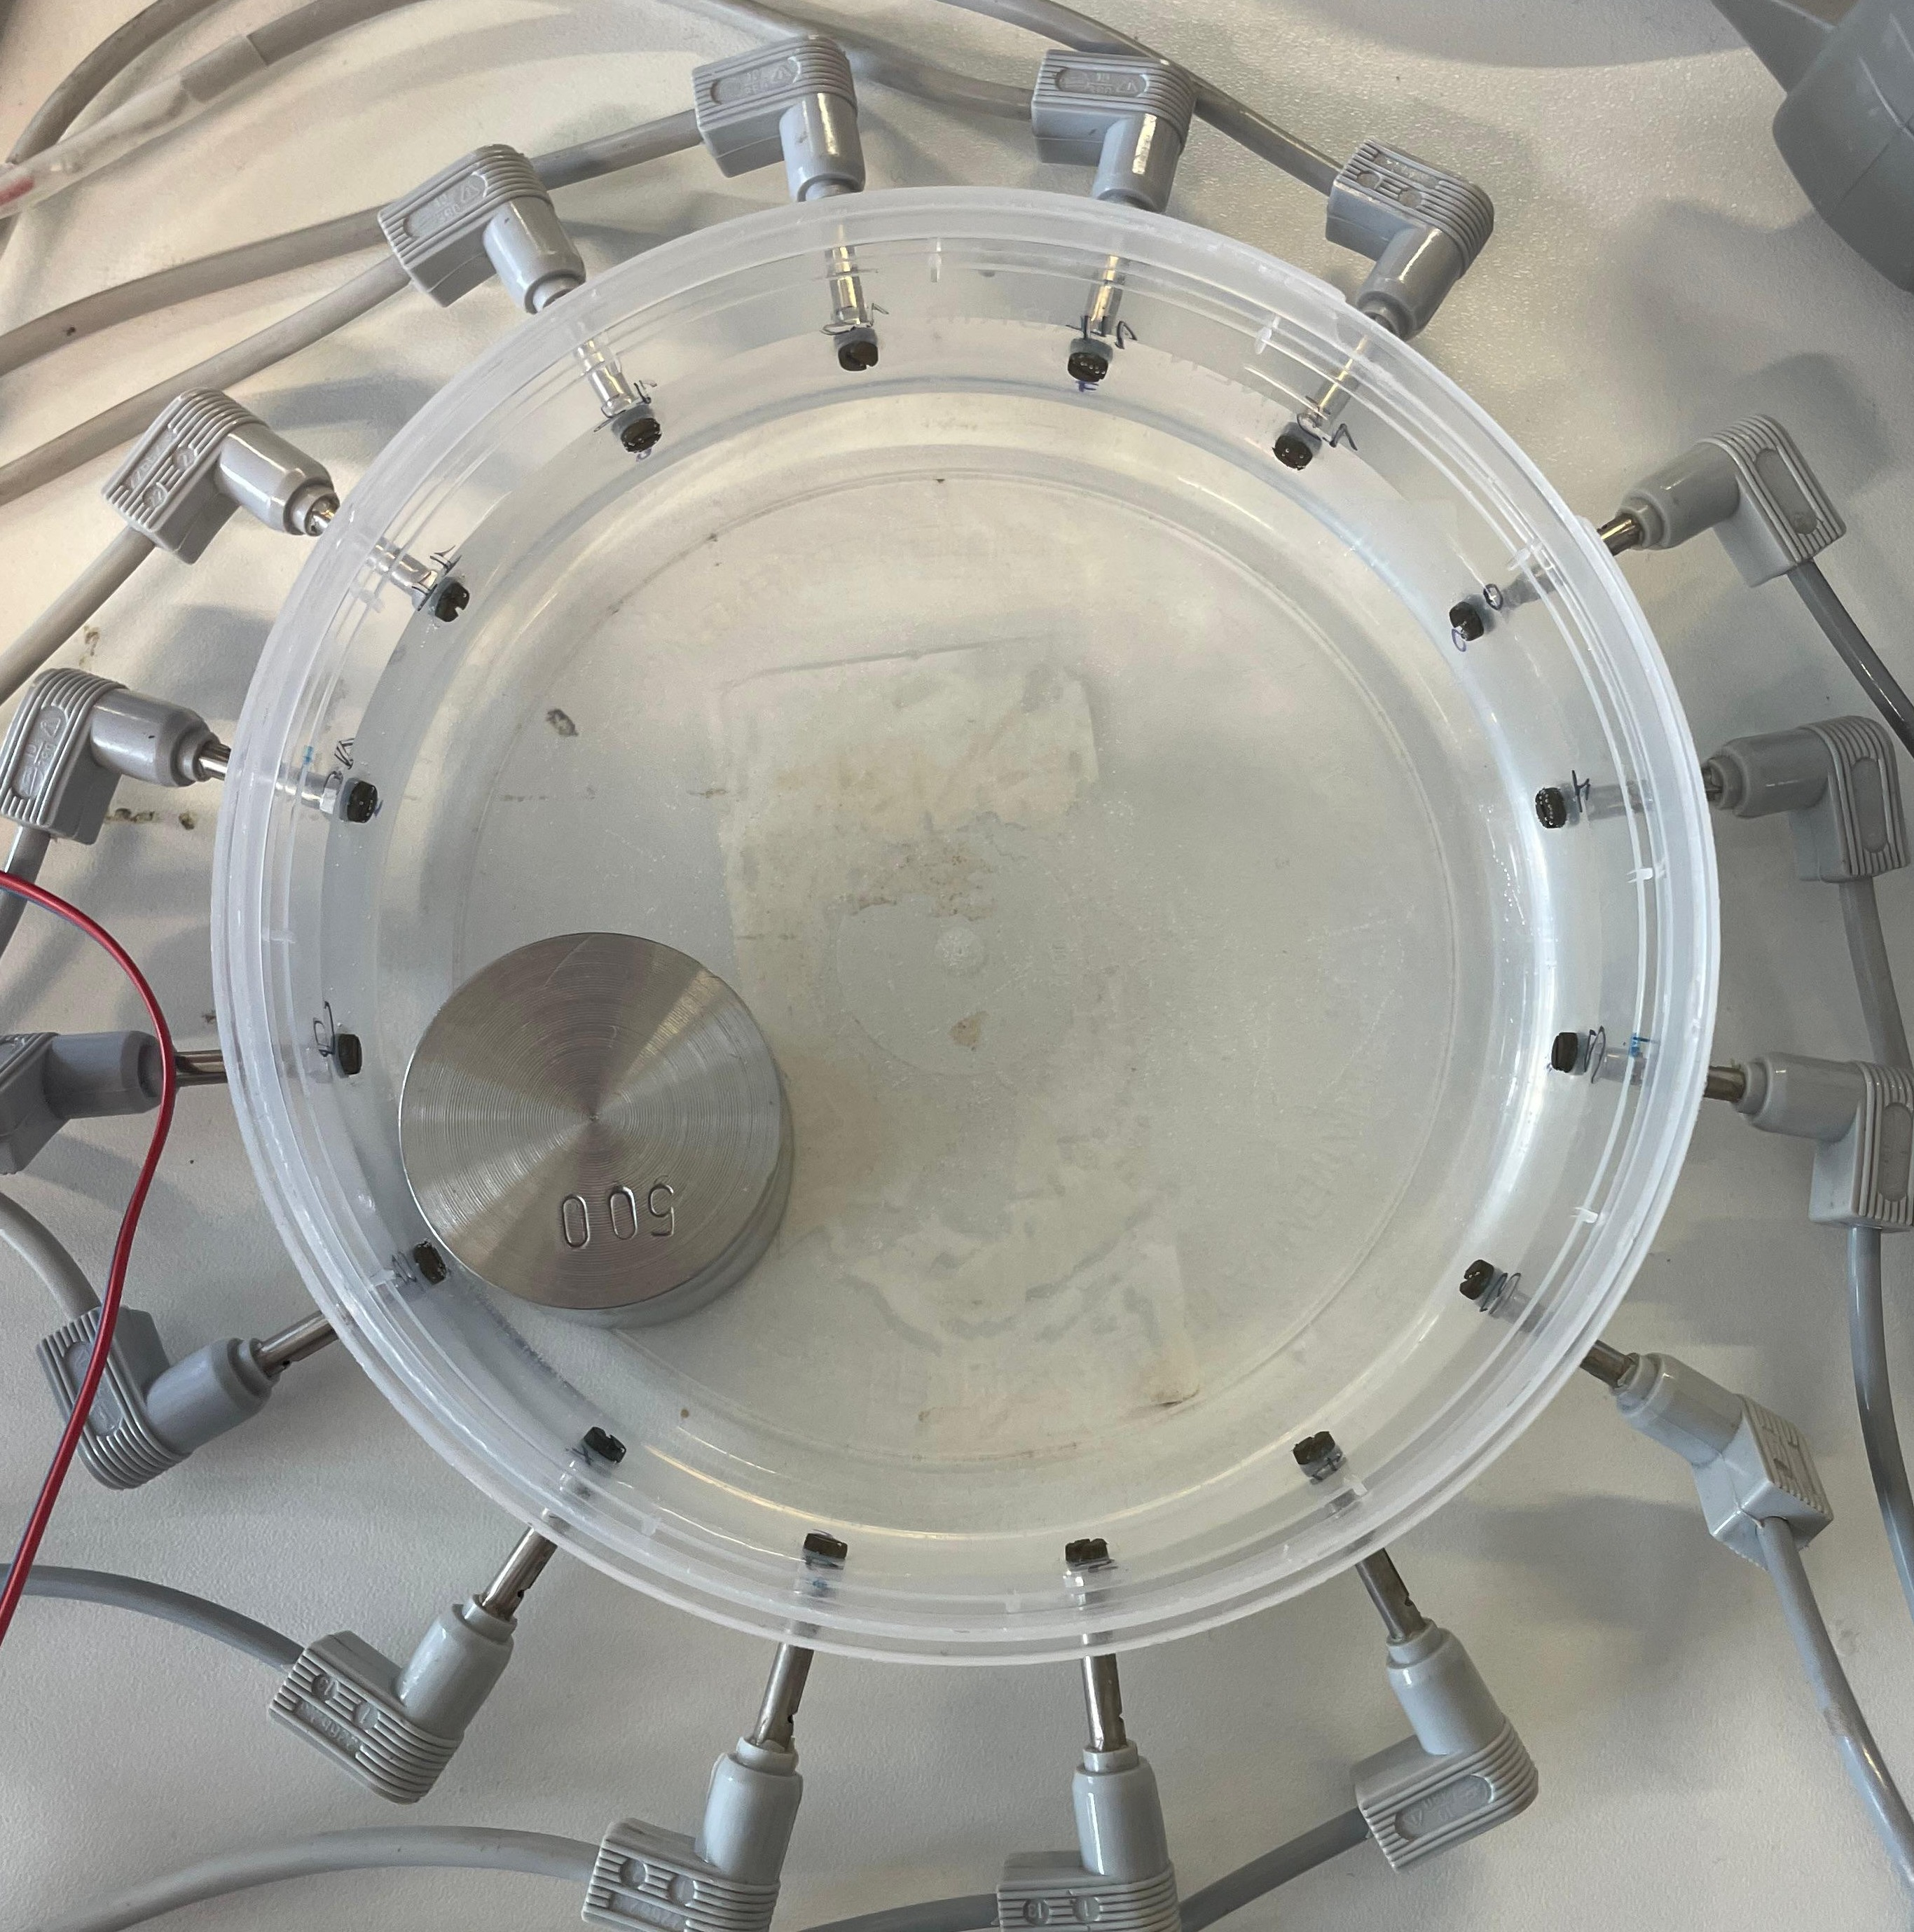
\includegraphics[width=\textwidth]{imagess/WhatsApp Image 2025-09-07 at 10.50.22_d7d43ed2.jpg} 
        \caption{Cylinder near electrode 0}
        \label{fig:cylinder_e0}
    \end{subfigure}
    \hspace{0.2\linewidth} % moderate space between images
    % Subfigure for position near electrode 7
    \begin{subfigure}[b]{0.31\linewidth}
        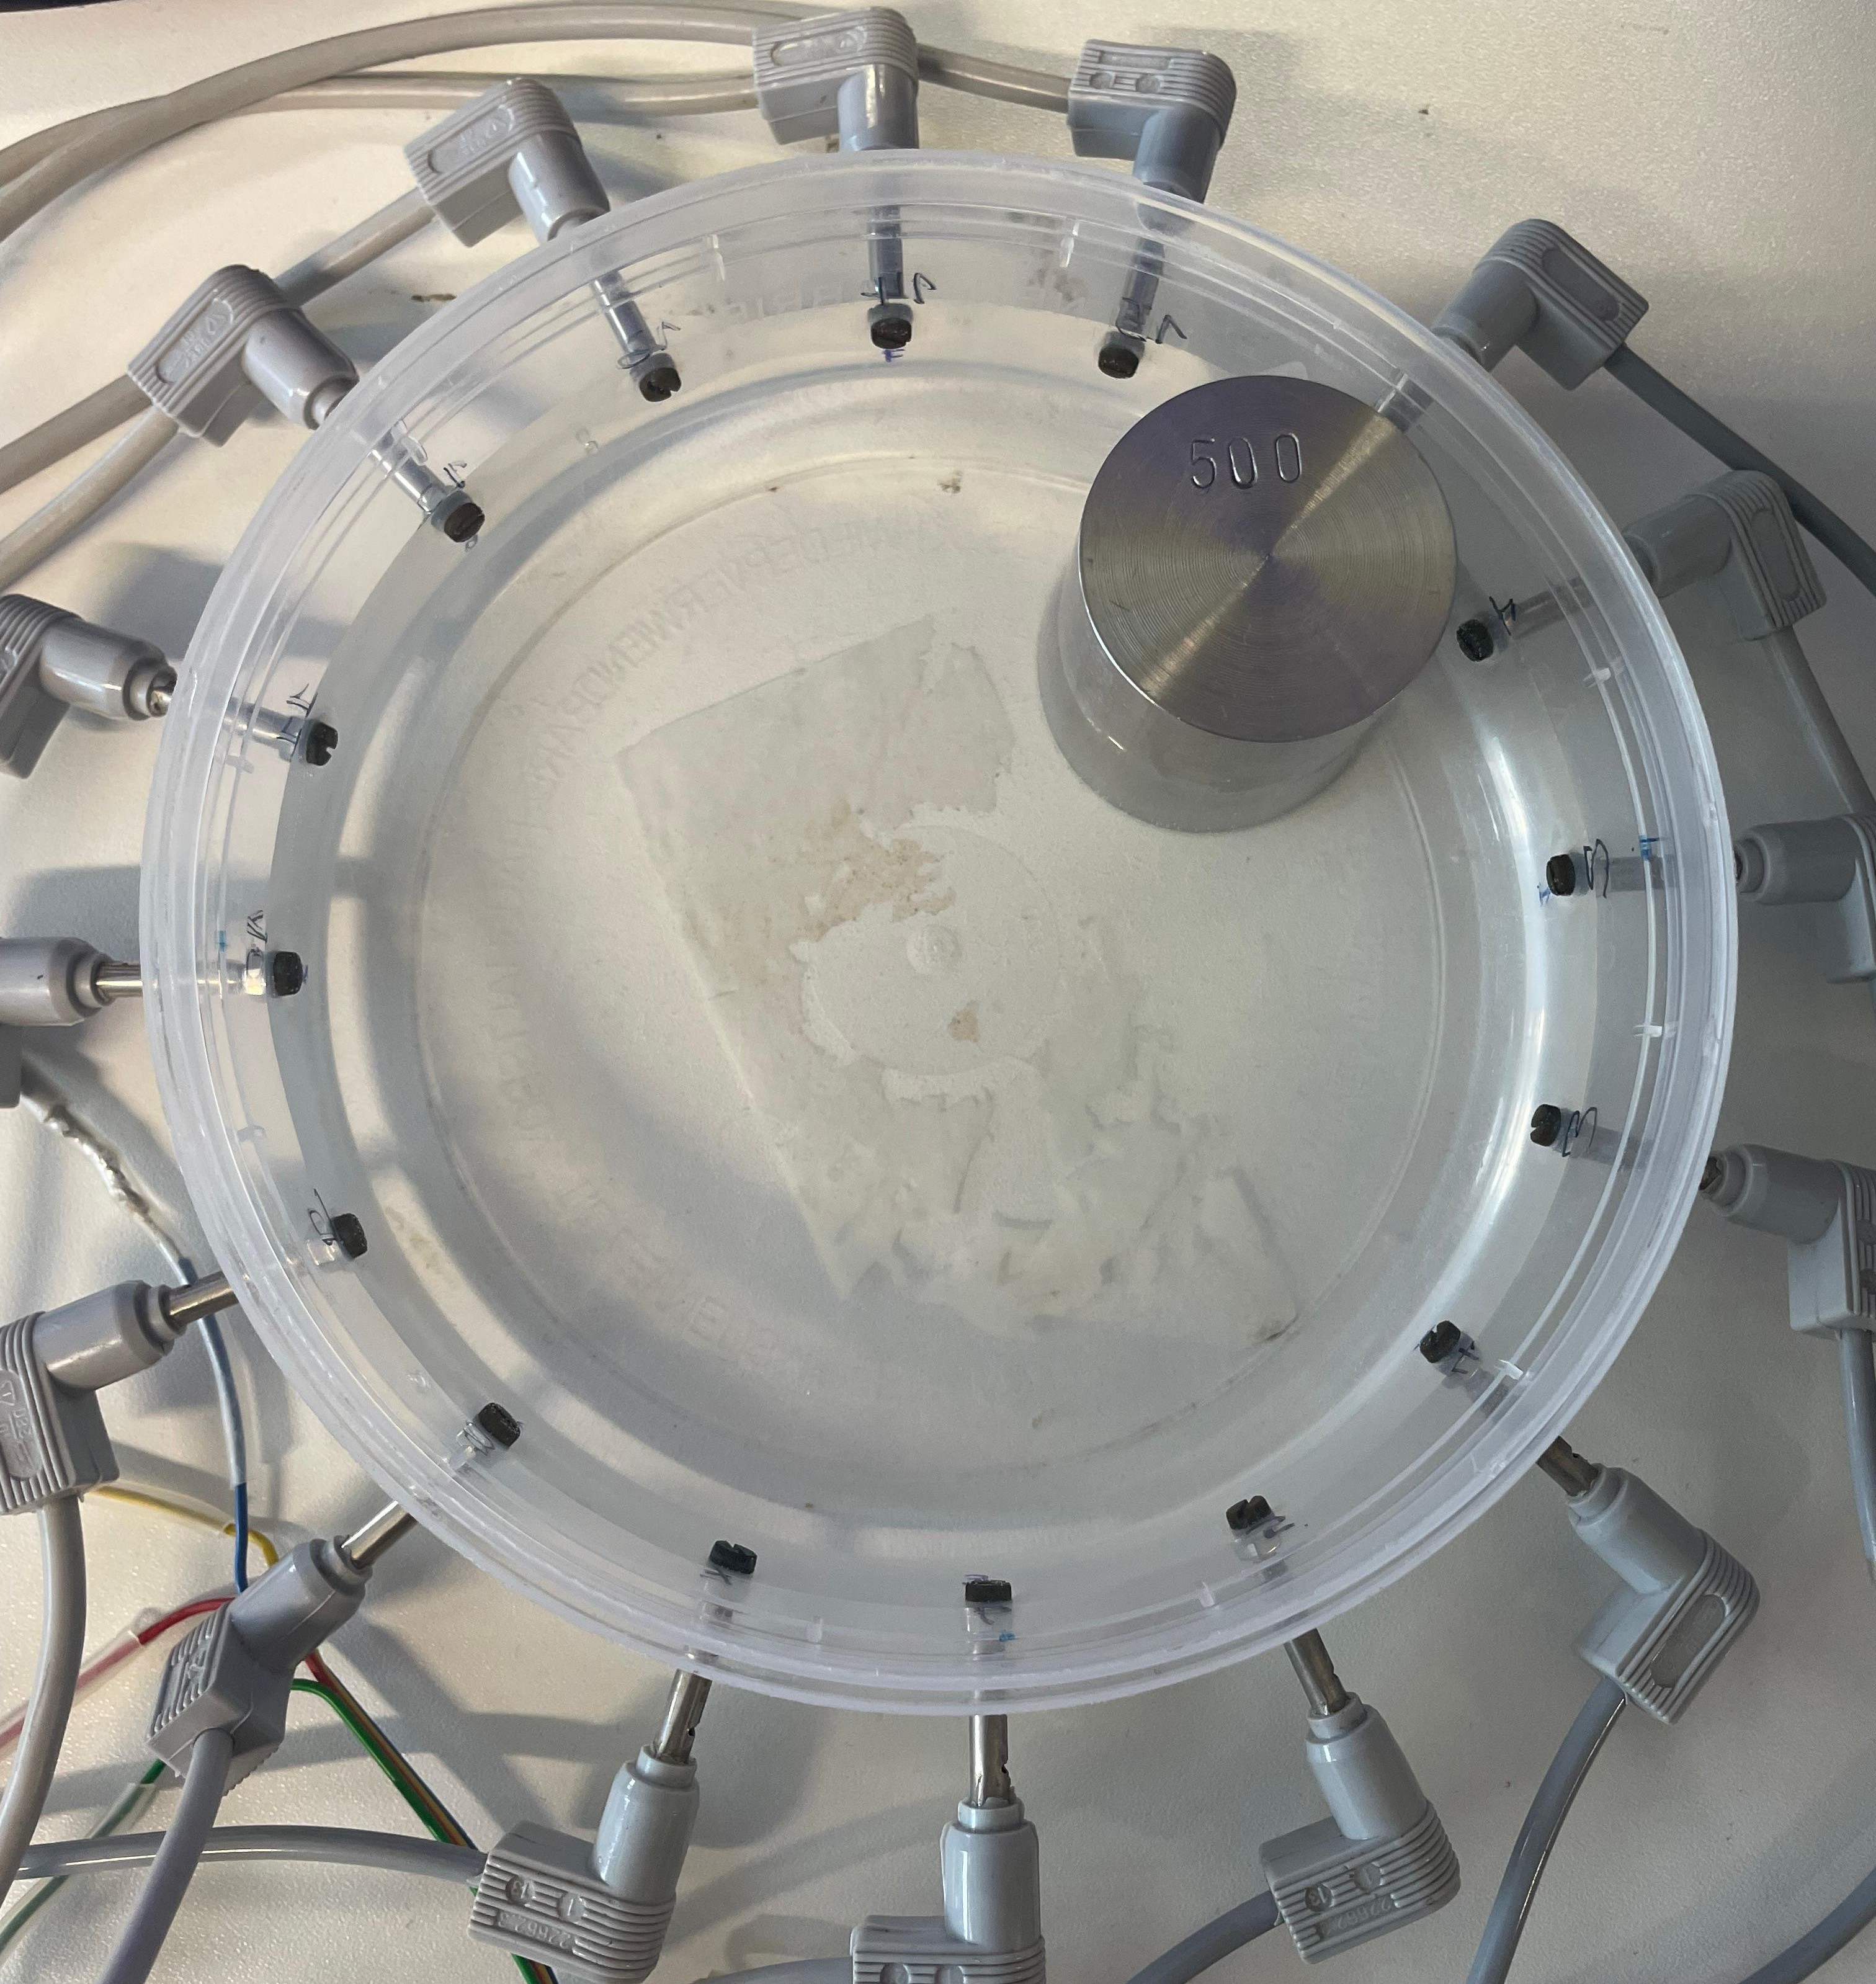
\includegraphics[width=\textwidth]{imagess/WhatsApp Image 2025-09-07 at 10.50.22_6e9b7119.jpg} 
        \caption{Cylinder near electrode 7}
        \label{fig:cylinder_e7}
    \end{subfigure}

    \caption{\footnotesize Experimental setup: water tank with a metallic cylindrical object in two different positions.}
    \label{fig:water_tank_setup_positions}
\end{figure}



  

% Explanatory sentence before the figure
Figure~\ref{fig:eit_recon_0} shows the reconstructed conductivity maps for a metallic object placed near electrode 0 
are shown below at two excitation frequencies.

\begin{figure}[H]
    \centering
    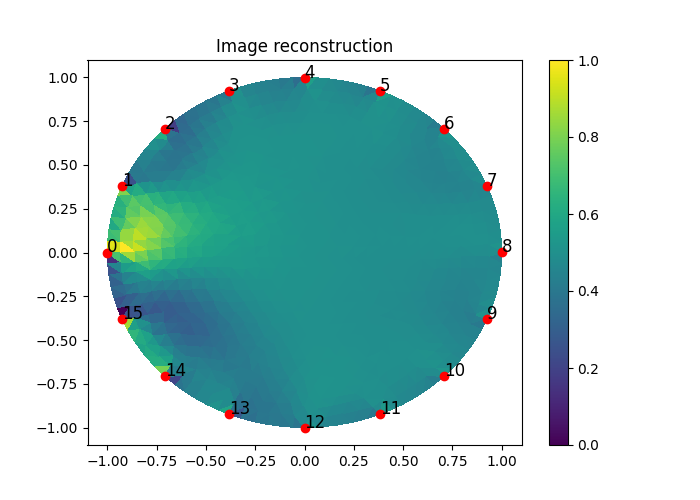
\includegraphics[width=0.45\linewidth]{imagess/figure0.png}
    \hfill
    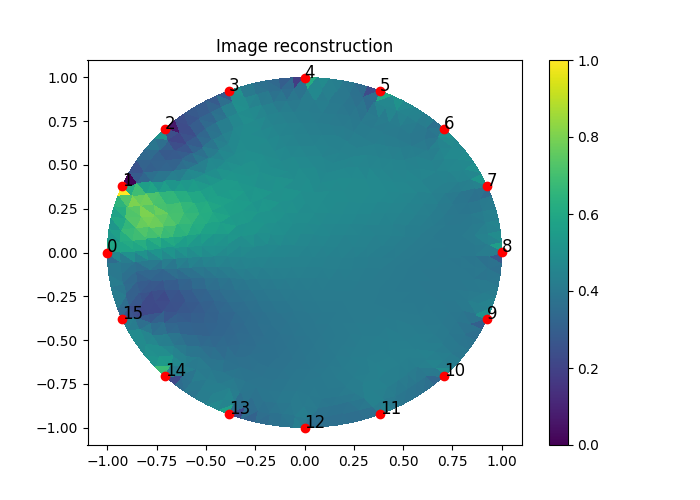
\includegraphics[width=0.45\linewidth]{imagess/Figure_44444444444444444.png}
    \caption{\footnotesize multi-frequency reconstructions of object near electrode 0: f = 9765.6250 kHz (left) and f = 49804.6875 kHz (right).}
    \label{fig:eit_recon_0}
\end{figure}

% Explanatory sentence before the figure
Figure~\ref{fig:eit_recon_7} reconstructed conductivity maps for a metallic object placed near electrode 7 
are shown below at two excitation frequencies.

\begin{figure}[H]
    \centering
    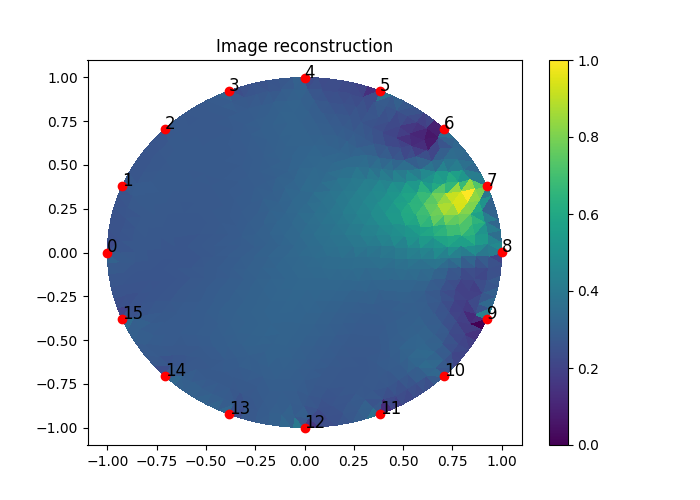
\includegraphics[width=0.45\linewidth]{imagess/electrode7777.png}
    \hfill
    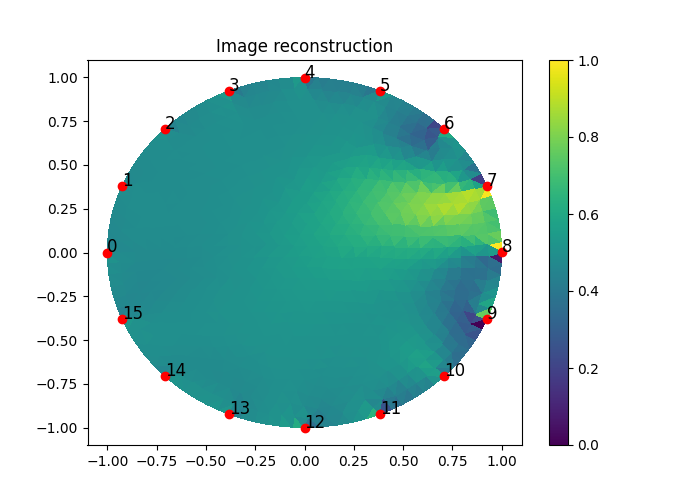
\includegraphics[width=0.45\linewidth]{imagess/electrode7.png}
    \caption{\footnotesize multi-frequency reconstructions of object near electrode 7: f = 9765.6250 kHz (left) and f = 49804.6875 kHz (right).}
    \label{fig:eit_recon_7}
\end{figure}

\subsubsection{Image reconstruction quality metrics}

Beyond visual inspection of the reconstructed conductivity maps, it is important to provide quantitative measures of image quality in order to assess the fidelity of the proposed system.

The Root Mean Squared Error (RMSE) can be computed between the reconstructed image and the reference experimental setup. This metric quantifies absolute pixel-level deviations and provides a direct measure of reconstruction accuracy\cite{adler2006uses}.

\begin{equation}
\text{RMSE} = \sqrt{\frac{1}{MN}\sum_{i=1}^{M}\sum_{j=1}^{N} \left(I_{ij}^{\text{recon}} - I_{ij}^{\text{ref}}\right)^2}
\end{equation}

The Signal-to-Noise Ratio (SNR) can be used also to evaluate the quality of the reconstructed image\cite{haase1991magnetic}:

\begin{equation}
\text{SNR} = \frac{\mu_{\text{signal}}}{\sigma_{\text{noise}}}
\end{equation}

These two metrics provide an objective basis to compare reconstructions across different experimental conditions and to evaluate the robustness of the imaging system.




\begin{table}[H]
\centering
\caption{Performance metrics for conductivity reconstruction at different positions and frequencies}
\label{tab:performance_metrics}
\begin{tabular}{|c|c|c|c|c|}
\hline
\textbf{Position} & \textbf{Electrode} & \textbf{Frequency (kHz)} & \textbf{RMSE} & \textbf{SNR (dB)} \\
\hline
Position 1 & Near Electrode 0 & 9765.6250 & $0.20$ & $28$ \\
\hline
Position 1 & Near Electrode 0 & 49804.6875 & $0.18$ & $32$ \\
\hline
Position 2 & Near Electrode 7 & 9765.6250 & $0.17$ & $22$ \\
\hline
Position 2 & Near Electrode 7 & 49804.6875 & $0.28$ & $32$ \\
\hline
\end{tabular}
\end{table}


\subsubsection{Multi-frequency EIT performance analysis}

Table~4.10 summarizes the performance metrics for conductivity reconstruction at two positions using low ($\sim 9.77$~kHz) and high ($\sim 49.8$~kHz) excitation frequencies. 
At the lower frequency, the Root Mean Squared Error (RMSE) is 0.20 near Electrode 0 (Position 1) and 0.17 near Electrode 7 (Position 2), with corresponding Signal-to-Noise Ratios (SNR) of 28~dB and 22~dB, respectively. 
Increasing the excitation frequency improves SNR across both positions (32~dB), indicating a stronger signal relative to measurement noise. 

These findings align with typical multi-frequency EIT behavior reported in the literature: higher excitation frequencies generally enhance signal quality but can lead to spatially non-uniform accuracy due to decreased sensitivity in regions distant from the electrodes. For instance, studies have shown that EIT systems operating at frequencies between 50 kHz and 250 kHz often achieve SNRs ranging from 25 dB to 35 dB, with RMSE values varying depending on the imaging protocol and system configuration which confirms the reliability and quality of the measurements.
\subsection{Experimental validation across 5 excitation frequencies}
Figure~\ref{fig:mf_reconstructions} presents the reconstructed images obtained after adjacent current injection in a water tank 
with a metallic cylindrical object placed near electrode 6 are shown below for 
five different excitation frequencies.
\begin{figure}[H]
    \centering
    % First row of images (3 images)
    \begin{subfigure}[b]{0.32\textwidth}
        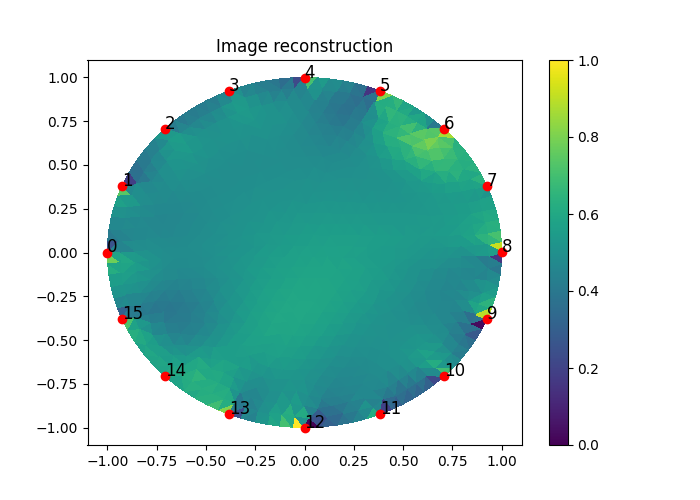
\includegraphics[width=\textwidth]{imagess/5f_3.png}
        \caption{Reconstruction at excitation frequency $f_1 = 9765.6250$ Hz}
    \end{subfigure}
    \hfill
    \begin{subfigure}[b]{0.32\textwidth}
        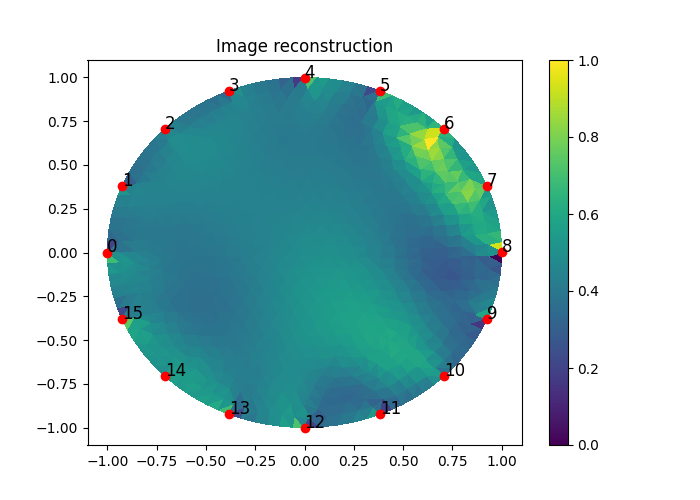
\includegraphics[width=\textwidth]{imagess/5f_2.png}
        \caption{Reconstruction at excitation frequency $f_2 = 22460.9375$ Hz}
    \end{subfigure}
    \hfill
    \begin{subfigure}[b]{0.32\textwidth}
        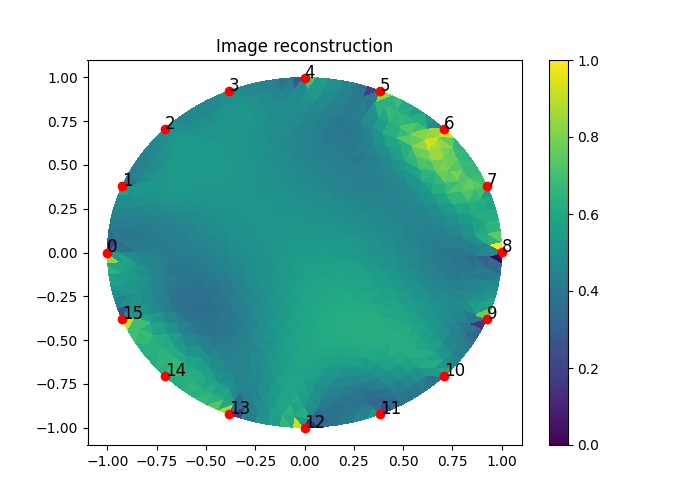
\includegraphics[width=\textwidth]{imagess/5f_1.png}
        \caption{Reconstruction at excitation frequency $f_3 = 49804.6875$ Hz}
    \end{subfigure}

    % Line break for second row
    \vskip\baselineskip

    % Second row of images (2 images, closer together)
    \begin{subfigure}[b]{0.32\textwidth}
        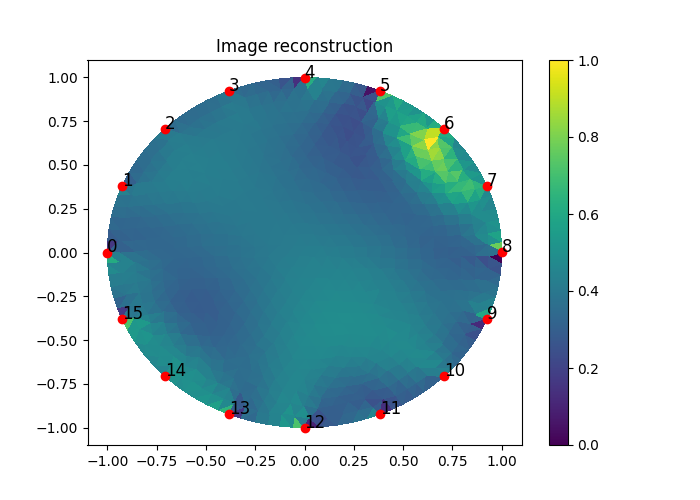
\includegraphics[width=\textwidth]{imagess/5f_4.png}
        \caption{Reconstruction at excitation frequency $f_4 = 111328.1250$ Hz}
    \end{subfigure}
    \hspace{1cm} % adjust this value for spacing between the two
    \begin{subfigure}[b]{0.32\textwidth}
        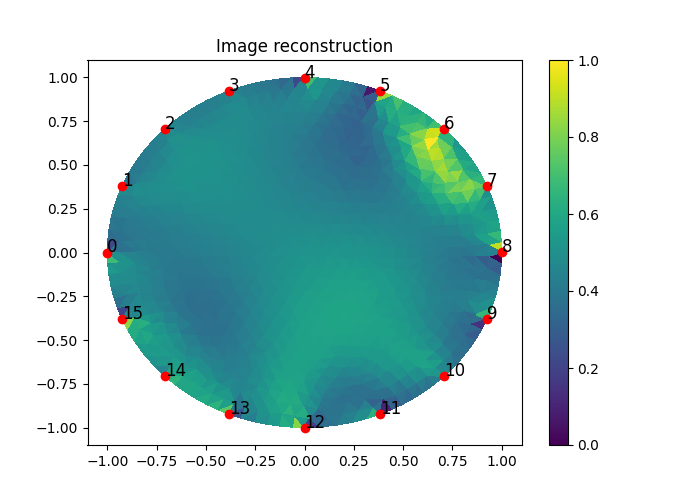
\includegraphics[width=\textwidth]{imagess/5f_5.png}
        \caption{Reconstruction at excitation frequency $f_5 = 250000.0000$ Hz}
    \end{subfigure}

    \caption{Multi-frequency reconstructions ($f_1$–$f_5$).}
    \label{fig:mf_reconstructions}
\end{figure}



As illustrated in Figure~\ref{fig:mf_reconstructions}, the reconstructed images correspond to the five excitation frequencies applied in the multi-frequency measurement. 
The metallic cylindrical object placed near electrode~6 is distinguishable in all reconstructions, appearing as a high-contrast region due to its significantly lower impedance compared to the surrounding saline water medium. 
However, the sharpness and localization of the reconstructed anomaly vary with frequency. At lower frequencies, the reconstructed object appears more diffused and less precisely localized, which can be attributed to the reduced sensitivity of adjacent current injection at low excitation frequencies. 
These results highlight the benefit of employing multi-frequency excitation for Electrical Impedance Tomography, as it provides complementary information across frequencies and allows for a more reliable identification of conductive inclusions in the imaging domain.\\
Although the metallic cylindrical object can be identified in the reconstructed images, the results are not perfectly accurate. 
The anomaly appears blurred and distorted, and its exact boundaries are difficult to delineate. 
This limitation can be mainly attributed to the intrinsic complexity of the EIT inverse problem, which is severely ill-posed and highly sensitive to modeling errors and measurement noise. 
Moreover, the use of multi-frequency excitation further increases the complexity of the reconstruction, since the tissue or medium response varies nonlinearly with frequency and requires accurate modeling of dispersive properties. The presence of boundary effects also reduces the achievable spatial resolution. 
As a result, while multi-frequency EIT provides complementary information, the reconstructions remain an approximation and must be interpreted with caution, highlighting the need for more advanced algorithms, better regularization strategies, and improved experimental setups to achieve higher fidelity images.




\section{Conclusion}
The frequency-domain measurements at an established resistance guaranteed that the EIT acquisition system yields stable and reproducible impedances over repeated trials. The experiment setup transferred this verification into the imaging domain. Reconstructed conductivity maps pinned down a metal object at different electrode positions and across multiple frequencies, showing the capability of the system to resolve spatial conductivity contrasts. Contrast between low- and high-frequency reconstructions is an indication of the complementary nature of multi-frequency excitation for higher image resolution and sensitivity.Overall, this chapter ensures the system built is stable in its impedance measurements and is capable of producing valid tomographic images, a sound foundation for further studies and uses of multi-frequency EIT.




\chapter*{General conclusion }
\markboth{General conclusion}{} %pour afficher l'entete
\addcontentsline{toc}{chapter}{General conclusion }

This project has addressed the design, implementation, and validation of a simultaneous multifrequency Electrical Impedance Tomography (EIT) acquisition system dedicated to biomedical applications. The developed platform, built around the STM32G474 microcontroller, successfully generated and acquired multifrequency excitation signals while ensuring reliable current and voltage measurements through carefully designed conditioning circuits. Signal processing methods such as Goertzel filtering and Fourier analysis were implemented to extract impedance values with high accuracy, and the system was validated through simulations, hardware experiments, and experimental measurements. The reproducibility tests confirmed that the acquisition chain provided stable results across repeated trials and different excitation frequencies, while image reconstruction experiments demonstrated the capability of the system to localize conductive inclusions inside a water test-tank. These results underline the feasibility of the proposed approach and highlight the advantages of simultaneous multifrequency operation compared to conventional sequential techniques.

Nevertheless, some limitations were encountered. At higher excitation frequencies, electrode polarization and parasitic effects introduced variability in the measurements, while the reconstructed images exhibited blurring and distortions that can be attributed to the intrinsic ill-posedness of the EIT inverse problem and to the simplified reconstruction algorithms employed. Despite these challenges, the overall system performance demonstrates the potential of simultaneous multifrequency EIT as a compact, low-cost, and versatile imaging modality for biomedical monitoring.

Looking ahead, future perspectives include the refinement of both hardware and software components in order to achieve higher accuracy and resolution. On the hardware side, improvements such as optimized analog front-end design, the use of higher-performance converters, and parallel multi-channel acquisition would allow better noise immunity and faster frame rates. On the algorithmic side, more advanced reconstruction methods, including nonlinear solvers and machine learning–based approaches, could enhance image quality and robustness against measurement uncertainties. Extending the frequency range of operation would further enable a more comprehensive characterization of tissue properties, while the integration of real-time processing pipelines would bring the system closer to clinical applicability. Finally, moving from controlled test-tank experiments toward in-vitro and in-vivo validation will be a crucial step in demonstrating the system’s practical relevance in medical diagnostics, rehabilitation monitoring, and human–machine interaction.

In conclusion, this work has established a functional proof of concept for a simultaneous multifrequency EIT system, demonstrating its reproducibility, robustness, and potential for biomedical imaging. By building upon the foundations laid in this thesis, future research can advance toward more accurate, reliable, and real-time EIT platforms capable of contributing meaningfully to next-generation healthcare technologies.

\renewcommand{\bibname}{References}
\bibliography{References}
\bibliographystyle{ieeetr} % or apalike, plainurl, etc.
\addcontentsline{toc}{chapter}{References}% ajouter son entrée dans la table

\includepdf[pages=-]{Document (13).pdf}
%\addcontentsline{toc}{chapter}{Acronymes}
\chapter*{List of Acronyms}
\addcontentsline{toc}{chapter}{List of Acronyms}

%%%%%% NB. Please ensure that the acronym list is maintained in alphabetical order.

\vspace{0.5cm}
\begin{itemize}
    \item \textbf{ADC:} Analog-to-Digital Converter
    \item \textbf{DAC:} Digital-to-Analog Converter
    \item \textbf{DAQ:} Data Acquisition
    \item \textbf{DMA:} Direct Memory Access
    \item \textbf{DSP:} Digital Signal Processor / Digital Signal Processing
    \item \textbf{EIT:} Electrical Impedance Tomography
    \item \textbf{FFT:} Fast Fourier Transform
    \item \textbf{FPGA:} Field Programmable Gate Array
    \item \textbf{GPIO:} General-Purpose Input/Output
    \item \textbf{HAL:} Hardware Abstraction Layer
    \item \textbf{I/Q:} In-phase / Quadrature
    \item \textbf{IEC:} International Electrotechnical Commission
    \item \textbf{MCU:} Microcontroller Unit
    \item \textbf{PCB:} Printed Circuit Board
    \item \textbf{RMSE:} Root Mean Squared Error
    \item \textbf{SNR:} Signal-to-Noise Ratio
    \item \textbf{TIM:} Timer (STM32 Peripheral)
    \item \textbf{VCCS:} Voltage-Controlled Current Source
    \item \textbf{Vpp:} Peak-to-Peak Voltage
\end{itemize}
\normalsize

\pagestyle{empty}

\renewcommand{\listtablename}{Tables}

% Fin du document
\end{document}
